\documentclass[12pt]{report}

% includes
\usepackage[a4paper, top=2cm, bottom=2cm, left=3cm, right=2cm]{geometry} % page size
\usepackage[utf8]{inputenc}     % encoding
\usepackage{palatino}           % font
\usepackage[romanian]{babel}    % language
\usepackage{graphicx}           % images
\usepackage{indentfirst}        % indentation
\usepackage[nottoc]{tocbibind}  % table of contents style
\usepackage[unicode]{hyperref}  % references from the table of contents
\usepackage{enumitem} % to customize lists
\setlist[1]{itemsep=-5pt}
\usepackage{csquotes} % needed dependency
\usepackage[backend=biber, natbib, style=apa]{biblatex} % bibliography
\addbibresource{bibliography.bib} % bibliography
\usepackage{listings} % for inline code
\usepackage{xcolor} % to define colors
\usepackage{float} % for figure placement
\usepackage{microtype} % improves typography
\usepackage{amsmath} % for math equations

\graphicspath{{images/}}        % path where the images are located
\setlength{\parindent}{1cm}     % paragraph indentation

% other options
\linespread{1.5}                % space between lines
\renewcommand*\contentsname{Cuprins}    % table of contents name

\definecolor{codegreen}{rgb}{0,0.6,0}
\definecolor{codegray}{rgb}{0.5,0.5,0.5}
\definecolor{codepurple}{rgb}{0.58,0,0.82}
\definecolor{backcolour}{rgb}{0.95,0.95,0.92}
\lstdefinestyle{mystyle}{
    backgroundcolor=\color{backcolour},   
    commentstyle=\color{codegreen},
    keywordstyle=\color{magenta},
    numberstyle=\tiny\color{codegray},
    stringstyle=\color{codepurple},
    basicstyle=\ttfamily\footnotesize,
    breakatwhitespace=false,         
    breaklines=true,                 
    captionpos=b,                    
    keepspaces=true,                 
    numbers=left,                    
    numbersep=5pt,                  
    showspaces=false,                
    showstringspaces=false,
    showtabs=false,                  
    tabsize=2
}
\lstset{style=mystyle}

% the document content
\begin{document}
    % macros (global)
    \newcommand{\university}    {Universitatea ``Alexandru-Ioan Cuza'' din Iași}
\newcommand{\universityg}   {Universității ``Alexandru-Ioan Cuza'' din Iași} % genitive
\newcommand{\faculty}       {Facultatea de Informatică}
\newcommand{\facultyg}      {Facultății de Informatică} % genitive
\newcommand{\speciality}    {informatică}
\newcommand{\promotion}     {2017–2020}                             %<---------

\newcommand{\thesistype}    {Lucrare de licență}
\newcommand{\thesistitle}   {Simularea funcționalităților unui mouse folosind repere faciale}    %<---------

\newcommand{\authorlast}    {Iacob}                               %<---------
\newcommand{\authorfirst}   {Sergiu}
\newcommand{\authornamefl}  {\authorfirst \space \authorlast} % first name first
\newcommand{\authornamelf}  {\authorlast \space \authorfirst} % last name first
\newcommand{\authorbirth}   {03 martie 1997}                      %<---------
\newcommand{\authoraddress} {România, jud. Iași, comuna Tomești, sat Tomești, strada Văzduh, nr. 73} %<---------
\newcommand{\authorcnp}     {1970301226742}                         %<---------

\newcommand{\session}       {iulie, 2020}                       %<---------
\newcommand{\coordinator}   {Asist. Dr. Croitoru Eugen}               %<---------

\newcommand{\dottedline}    {............................}
    
    % front-matter
    \pagenumbering{gobble}
    
    % define the cover page
\begin{titlepage}
    \begin{center}
        % the university and faculty
        \large
        \MakeUppercase{\university}
        
        \LARGE
        \textbf{\MakeUppercase{\faculty}}
        
        % the faculty logo
        \vspace{1cm}
        
\includegraphics[width=0.3\textwidth]{logoFii.png}
        
        % thesis title
        \vspace{1cm}
        \Large
        \MakeUppercase{\thesistype}
        
        \vspace{0.5cm}
        \LARGE
        \textbf{\thesistitle}
        
        % author
        \vspace{2cm}
        \Large
        propusă de
        
        \vspace{0.5cm}
        \LARGE
        \textbf{\authornamefl}
        
        % session
        \vfill
        \Large
        \textbf{Sesiunea:} \session
        
        % scientific coordinator
        \vspace{2cm}
        \Large
        Coordonator științific
        
        \vspace{0.5cm}
        \LARGE
        \textbf{\coordinator}
    \end{center}
\end{titlepage}
    % define the title page
\begin{titlepage}
    \begin{center}
        % the university and faculty
        \large
        \MakeUppercase{\university}
        
        \LARGE
        \textbf{\MakeUppercase{\faculty}}
        
        % thesis title
        \vspace{8cm}
        \huge
        \textbf{\thesistitle}
        
        % author
        \vspace{2cm}
        \LARGE
        \textbf{\authornamefl}
        
        % session
        \vfill
        \Large
        \textbf{Sesiunea:} \session
        
        % scientific coordinator
        \vspace{4cm}
        \Large
        Coordonator științific
        
        \vspace{0.5cm}
        \LARGE
        \textbf{\coordinator}
    \end{center}
\end{titlepage}
    \cleardoublepage
    % \vspace*{\fill}

\begin{flushright}
    Avizat, \\
    Îndrumător lucrare de licență, \\
    \coordinator. \\
    Data: \dottedline \hspace{1cm} Semnătura: \dottedline
\end{flushright}

\vspace{1cm}
\begin{center}
    \large
    \textbf{Declarație privind originalitatea conținutului lucrării de licență}
\end{center}

Subsemnatul \textbf{\authornamelf} domiciliat în \textbf{\authoraddress}, născut la data de \textbf{\authorbirth}, identificat prin CNP \textbf{\authorcnp}, absolvent al \facultyg, \textbf{\faculty} specializarea \textbf{\speciality}, promoția \promotion, declar pe propria răspundere cunoscând consecințele falsului în declarații în sensul art. 326 din Noul Cod Penal și dispozițiile Legii Educației Naționale nr. 1/2011 art. 143 al. 4 și 5 referitoare la plagiat, că lucrarea de licență cu titlul \textbf{\thesistitle} elaborată sub îndrumarea domnului \textbf{\coordinator}, pe care urmează să o susțin în fața comisiei este originală, îmi aparține și îmi asum conținutul său în întregime.

De asemenea, declar că sunt de acord ca lucrarea mea de licență să fie verificată prin orice modalitate legală pentru confirmarea originalității, consimțind inclusiv la introducerea conținutului ei într-o bază de date în acest scop.

Am luat la cunoștință despre faptul că este interzisă comercializarea de lucrări științifice în vederea facilitării falsificării de către cumpărător a calității de autor al unei lucrări de licență, de diplomă sau de disertație și în acest sens, declar pe proprie răspundere că lucrarea de față nu a fost copiată ci reprezintă rodul cercetării pe care am întreprins-o.

\begin{flushright}
    Data: \dottedline \hspace{6cm} Semnătura: \dottedline
\end{flushright}

\vspace*{\fill}
\pagebreak
    % \vspace*{\fill}
\begin{center}
    \large
    \textbf{Declarație de consimțământ}
\end{center}

Prin prezenta declar că sunt de acord ca lucrarea de licență cu titlul \textbf{\thesistitle}, codul sursă al programelor și celelalte conținuturi (grafice, multimedia, date de test, etc.) care însoțesc această lucrare să fie utilizate în cadrul \facultyg.

De asemenea, sunt de acord ca \faculty \space de la \university, să utilizeze, modifice, reproducă și să distribuie în scopuri necomerciale programele-calculator, format executabil și sursă, realizate de mine în cadrul prezentei lucrări de licență.

\begin{flushright}
    Absolvent \textbf{\authornamefl} \\
    \vspace{0.5cm}
    Data: \dottedline \hspace{6cm} Semnătura: \dottedline
\end{flushright}
\vspace*{\fill}
\pagebreak
    
    % table of contents
    \tableofcontents
    
    % chapters
    \setcounter{page}{1}
    \pagenumbering{arabic}
    
    % \chapter*{Motivație} 
\addcontentsline{toc}{chapter}{Motivație}
    \chapter*{Introducere} 
\addcontentsline{toc}{chapter}{Introducere}

\section*{Context}
\addcontentsline{toc}{section}{Context}

Știință și tehnologie.
Acest duo se regăsește la orice pas al secolului XXI și interacționăm cu el zilnic, mai mult sau mai puțin, prin intermediul multor dispozitive precum telefonul, televizorul sau calculatorul personal.
Într-o formă sau alta, dispozitivele de acest fel (\emph{împreună} cu mulțimea de aplicații software pe care le rulează) fac lumea mai \emph{accesibilă} pentru utilizatorii lor – de pildă, să verificăm vremea zilei de mâine pe un laptop sau să ne bazăm pe comenzile online în timpul unei pandemii.
Astfel de exemple ne arată cum tehnologia modelează felul în care ne desfășurăm activitățile zilnice și ``scurtăturile'' pe care le putem lua pentru a îndeplini anumite sarcini – desigur, în anumite cazuri, cu niște costuri aferente.

În paragraful de mai sus este accentuat termenul ``accesibil'' care, prin definiție\footnote{Definiție preluată din DEX 2009}, înseamnă ceva ``care este la îndemâna cuiva; care poate fi ușor procurat''.
Am văzut cum lumea poate fi ``mai la îndemâna cuiva'' – dar cum facem ca tehnologia să fie, la rândul ei, accesibilă?
Cum ar putea, spre exemplu, o persoană paralizată să folosească un laptop?

După o analiză retrospectivă putem constata că oamenii au lucrat dintotdeauna la modalități (de exemplu la dezvoltarea de software) pentru a face tehnologia mai accesibilă oamenilor.
Un exemplu ar fi ``Cititorul de ecran'' (în engleză ``Screen reader''), care este incorporat în majoritatea smartphone-urilor recent lansate, sau asistentul inteligent precum Siri, Bixby sau Google Assistant.
Acestea pot permite persoanelor fără vedere să interpreteze conținutul unui ecran digital sau unei persoane imobilizate să asculte muzică, să afle noutăți ș.a.m.d.
Acest tip de software este un factor cheie pentru a permite unor categorii diverse de oameni să poată profita de avantajele tehnologiei.

\section*{Idee}
\addcontentsline{toc}{section}{Idee}

Dacă este să analizăm laptop-urile care sunt acum pe piață, am constata că toate sunt echipate cu o cameră frontală de luat vederi pentru videoconferințe, denumită uzual \emph{webcam}.
Pentru calculatoarele obișnuite, precum un ``sistem desktop'' cu un monitor care nu dispune de această cameră integrată, exista webcam-uri care se pot conecta printr-un port USB (de cele mai multe ori) și aduc aceeași funcționalitate și unui calculator ``tradițional''.

\begin{figure}[h]
    \centering
    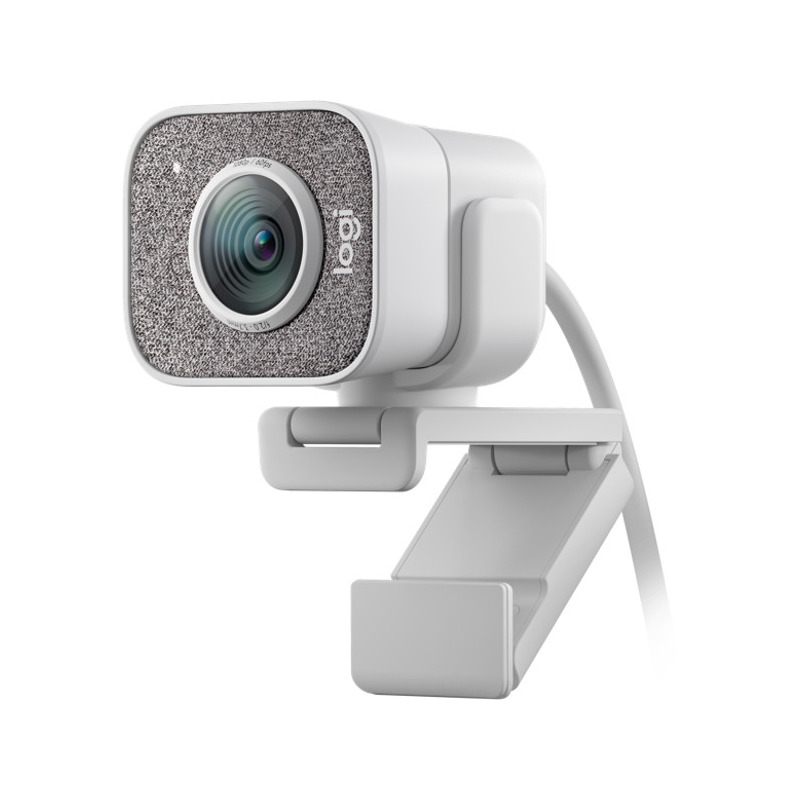
\includegraphics[width=0.3\textwidth]{webcam.jpg}
    \caption{Exemplu de webcam ce poate fi montat pe monitorul unui calculator. Imagine preluată de pe \href{https://www.pcgarage.ro/camere-web/logitech/streamcam-off-white/}{PC Garage}}
\end{figure}

Lucrarea de față ia în considerare popularitatea acestui webcam și propune o soluție pentru a putea folosi parțial un calculator fără ajutorul mâinilor.
O mare parte din interacțiunea dintre om și calculator se petrece \emph{prin intermediul mouse-ului}, așadar m-am concentrat pe simularea comportamentului acestuia \emph{folosind doar caracteristici ale feței}.
Ideea de bază constă în a prelua imagini ale utilizatorului de la webcam și, pe baza trăsăturilor faciale, de a simula funcționalități ale acestuia, spre exemplu de a muta cursorul în direcția în care privește utilizatorul.
Exemplul cel din urmă este cunoscut în litera științifică drept \emph{``Urmărirea ochilor''} (din engleză, \emph{``Eye tracking''}) și problema poate fi abordată prin tehnici de \emph{Învățare Automată}, o ramură a \emph{Inteligenței Artificiale}.

\begin{figure}[h]
    \centering
    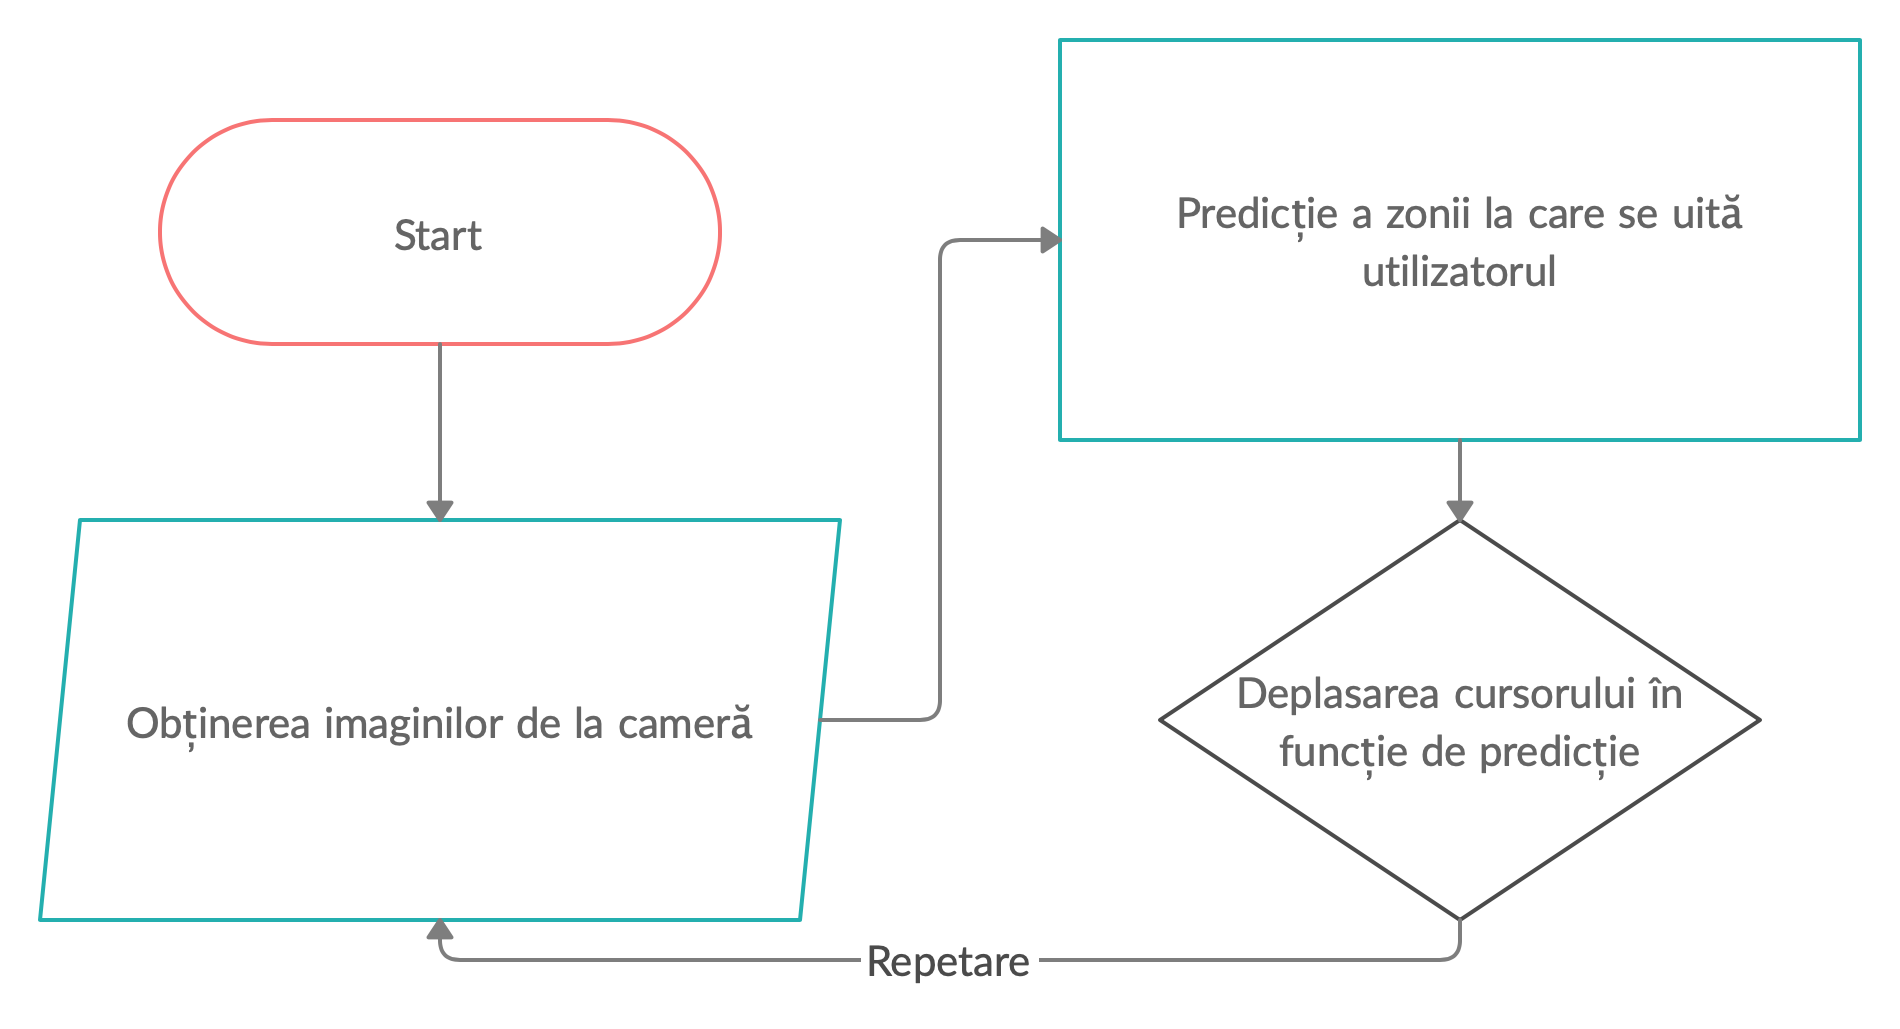
\includegraphics[width=\textwidth]{idee.png}
    \caption{Idee inițială pentru deplasarea cursorului}
\end{figure}

Această idee nu este nouă și există deja soluții pentru această problemă, bazate pe aceeași idee.
Totuși, cele mai multe dintre ele sunt create ori doar pentru un anumit sistem de operare (în acest caz, Windows), ori nu sunt gratuite și au un cost atașat semnificativ, sau chiar necesită componente hardware adiționale.

\emph{Camera Mouse}\footnote{\url{http://www.cameramouse.org}} este o propunere viabilă care urmărește o porțiune fixată a feței (spre exemplu vârful nasului) și, când acea porțiune își schimbă poziția, se schimbă și poziția cursorului.
Pentru ca acest lucru să funcționeze, utilizatorul trebuie să efectueze mișcări ale capului.
Oferă și functionalități de simulare a apăsării pe butoanele mouse-ului, însă aplicația funcționează doar pentru sistemele care rulează Windows.
Printre alternative se mai găsesc \emph{IntelliGaze}\footnote{\url{https://www.intelligaze.com/en/}} și produse dezvoltate de \emph{Tobii Dynavox}\footnote{\url{https://www.tobiidynavox.com/software/windows-software/windows-control-2/}}, dar acestea necesită în primul rând hardware adițional, lucrează doar pentru sistemul de operare Windows și au și un cost atașat.

\section*{Motivație}
\addcontentsline{toc}{section}{Motivație}

Când a trebuit să mă decid asupra temei lucrării de licență, am luat în calcul doi factori cheie: viitoarea mea carieră profesională și utilitatea proiectului.
Mi-am dorit să lucrez la un proiect care mi-ar alimenta interesul în Inteligența Artificială și care mi-ar oferi șansa de a aplica cercetarea pe care aș face-o în acest domeniu.
Mai mult, mi-am dorit de asemenea să am și o abordare practică asupra lucrării, astfel încât să construiesc ceva ce ar fi folositor.

Cât despre Inteligența Artificială, este inutil să-i subliniem importanța contemporană.
De la aplicabilitatea medicală, conducere/pilotare autonomă, agricultură inteligentă până la frigidere inteligente care-ți spun când ai rămas fără lapte, Inteligența Artificială este larg răspândită și extinderea ei nu se va opri prea curând.
Pentru mine, acesta este un motiv în plus pentru a o studia și a o înțelege mai bine, mai ales că o găsim integrată în viața noastră de zi cu zi.

\section*{Obiective}
\addcontentsline{toc}{section}{Obiective}

Cel mai important obiectiv al acestei lucrări de licență este înțelegerea și aplicarea cu succes a cunoștințelor și a noțiunilor dobândite ca student al \facultyg.
Câteva exemple de concepte de care am ținut cont sunt legate de principii de \emph{software design} (precum principiile de programare \emph{SOLID}), de concepte de analizare a complexității timp/spațiu sau de noțiuni matematice legate de învățarea automată.
Toate aceste noțiuni, teoretice și practice, trebuie să se regăsească într-o combinație armonioasă pentru a putea permite dezvoltarea unui software de calitate.

Obiectivul principal al aplicației este acela de a simula folosirea unui mouse doar prin gesturi ale feței.
Așadar, mai jos este o listă a celor mai importante funcționalități ale acestuia pe care mi-am propus să le replic prin această lucrare:
\begin{itemize}
    \item mișcarea cursorului
    \item apăsarea butonului stâng
    \item apăsarea butonului drept\footnote{Aceste funcționalități mai sunt denumite uzual și ``click stânga/dreapta''}
\end{itemize}

\begin{figure}[h]
    \centering
    
\includegraphics[width=0.5\textwidth]{mouse.png}
    \caption{Funcționalități principale ale unui mouse. Imagine preluată și adaptată de pe \href{https://www.flaticon.com}{Flaticon}, autor: \href{https://www.flaticon.com/authors/kiranshastry}{Kiranshastry}}
\end{figure}

\section*{Metodologie}
\addcontentsline{toc}{section}{Metodologie}

\section*{Descriere sumară a soluției}
\addcontentsline{toc}{section}{Descriere sumară a soluției}

Fața umană poate fi analizată pe baza mai multor \emph{repere faciale}.
Acestea sunt reprezentate prin anumite puncte de pe față precum centrul ochiului, centrul nasului, centrul buzei superioare etc.
Cunoscând acestea, putem delimita zone ale feței precum un singur ochi.
În figura de mai jos\ref{figure:facial-landmarks}, ochiul stâng al unei persoane este delimitat de înfășurătoarea convexă a punctelor cu indicii $[43, 48]$.

\begin{figure}[h]
    \centering
    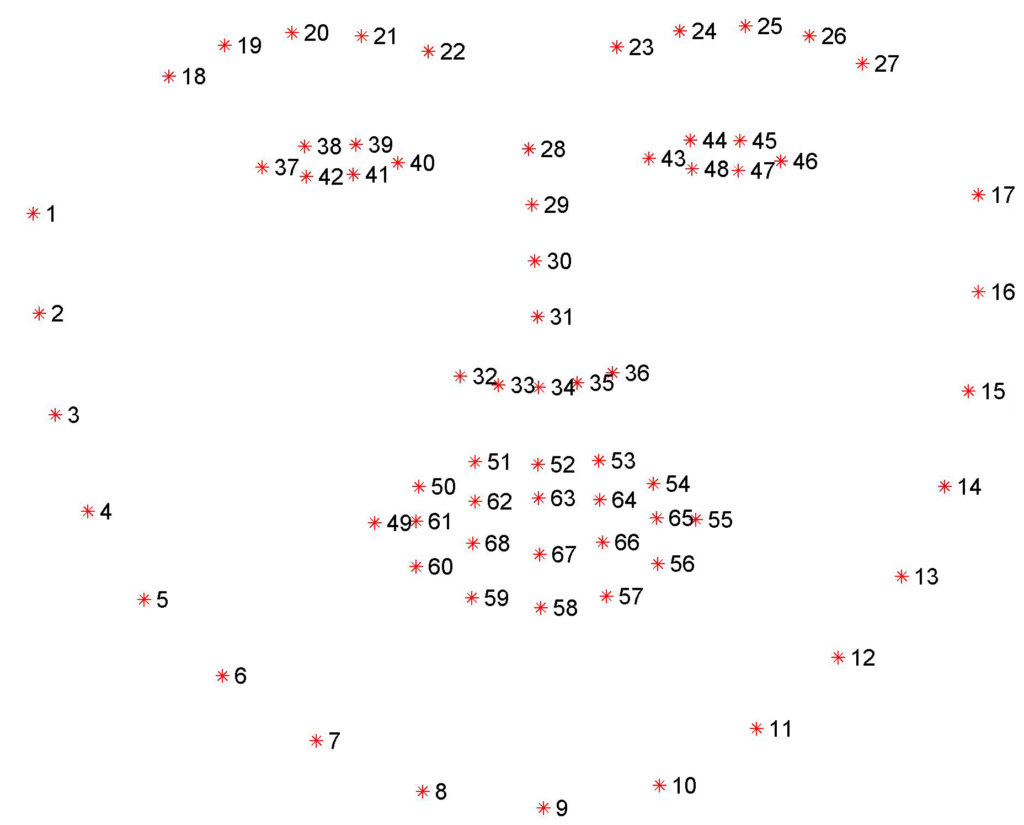
\includegraphics[width=0.49\textwidth]{facial_landmarks_1.jpg}
    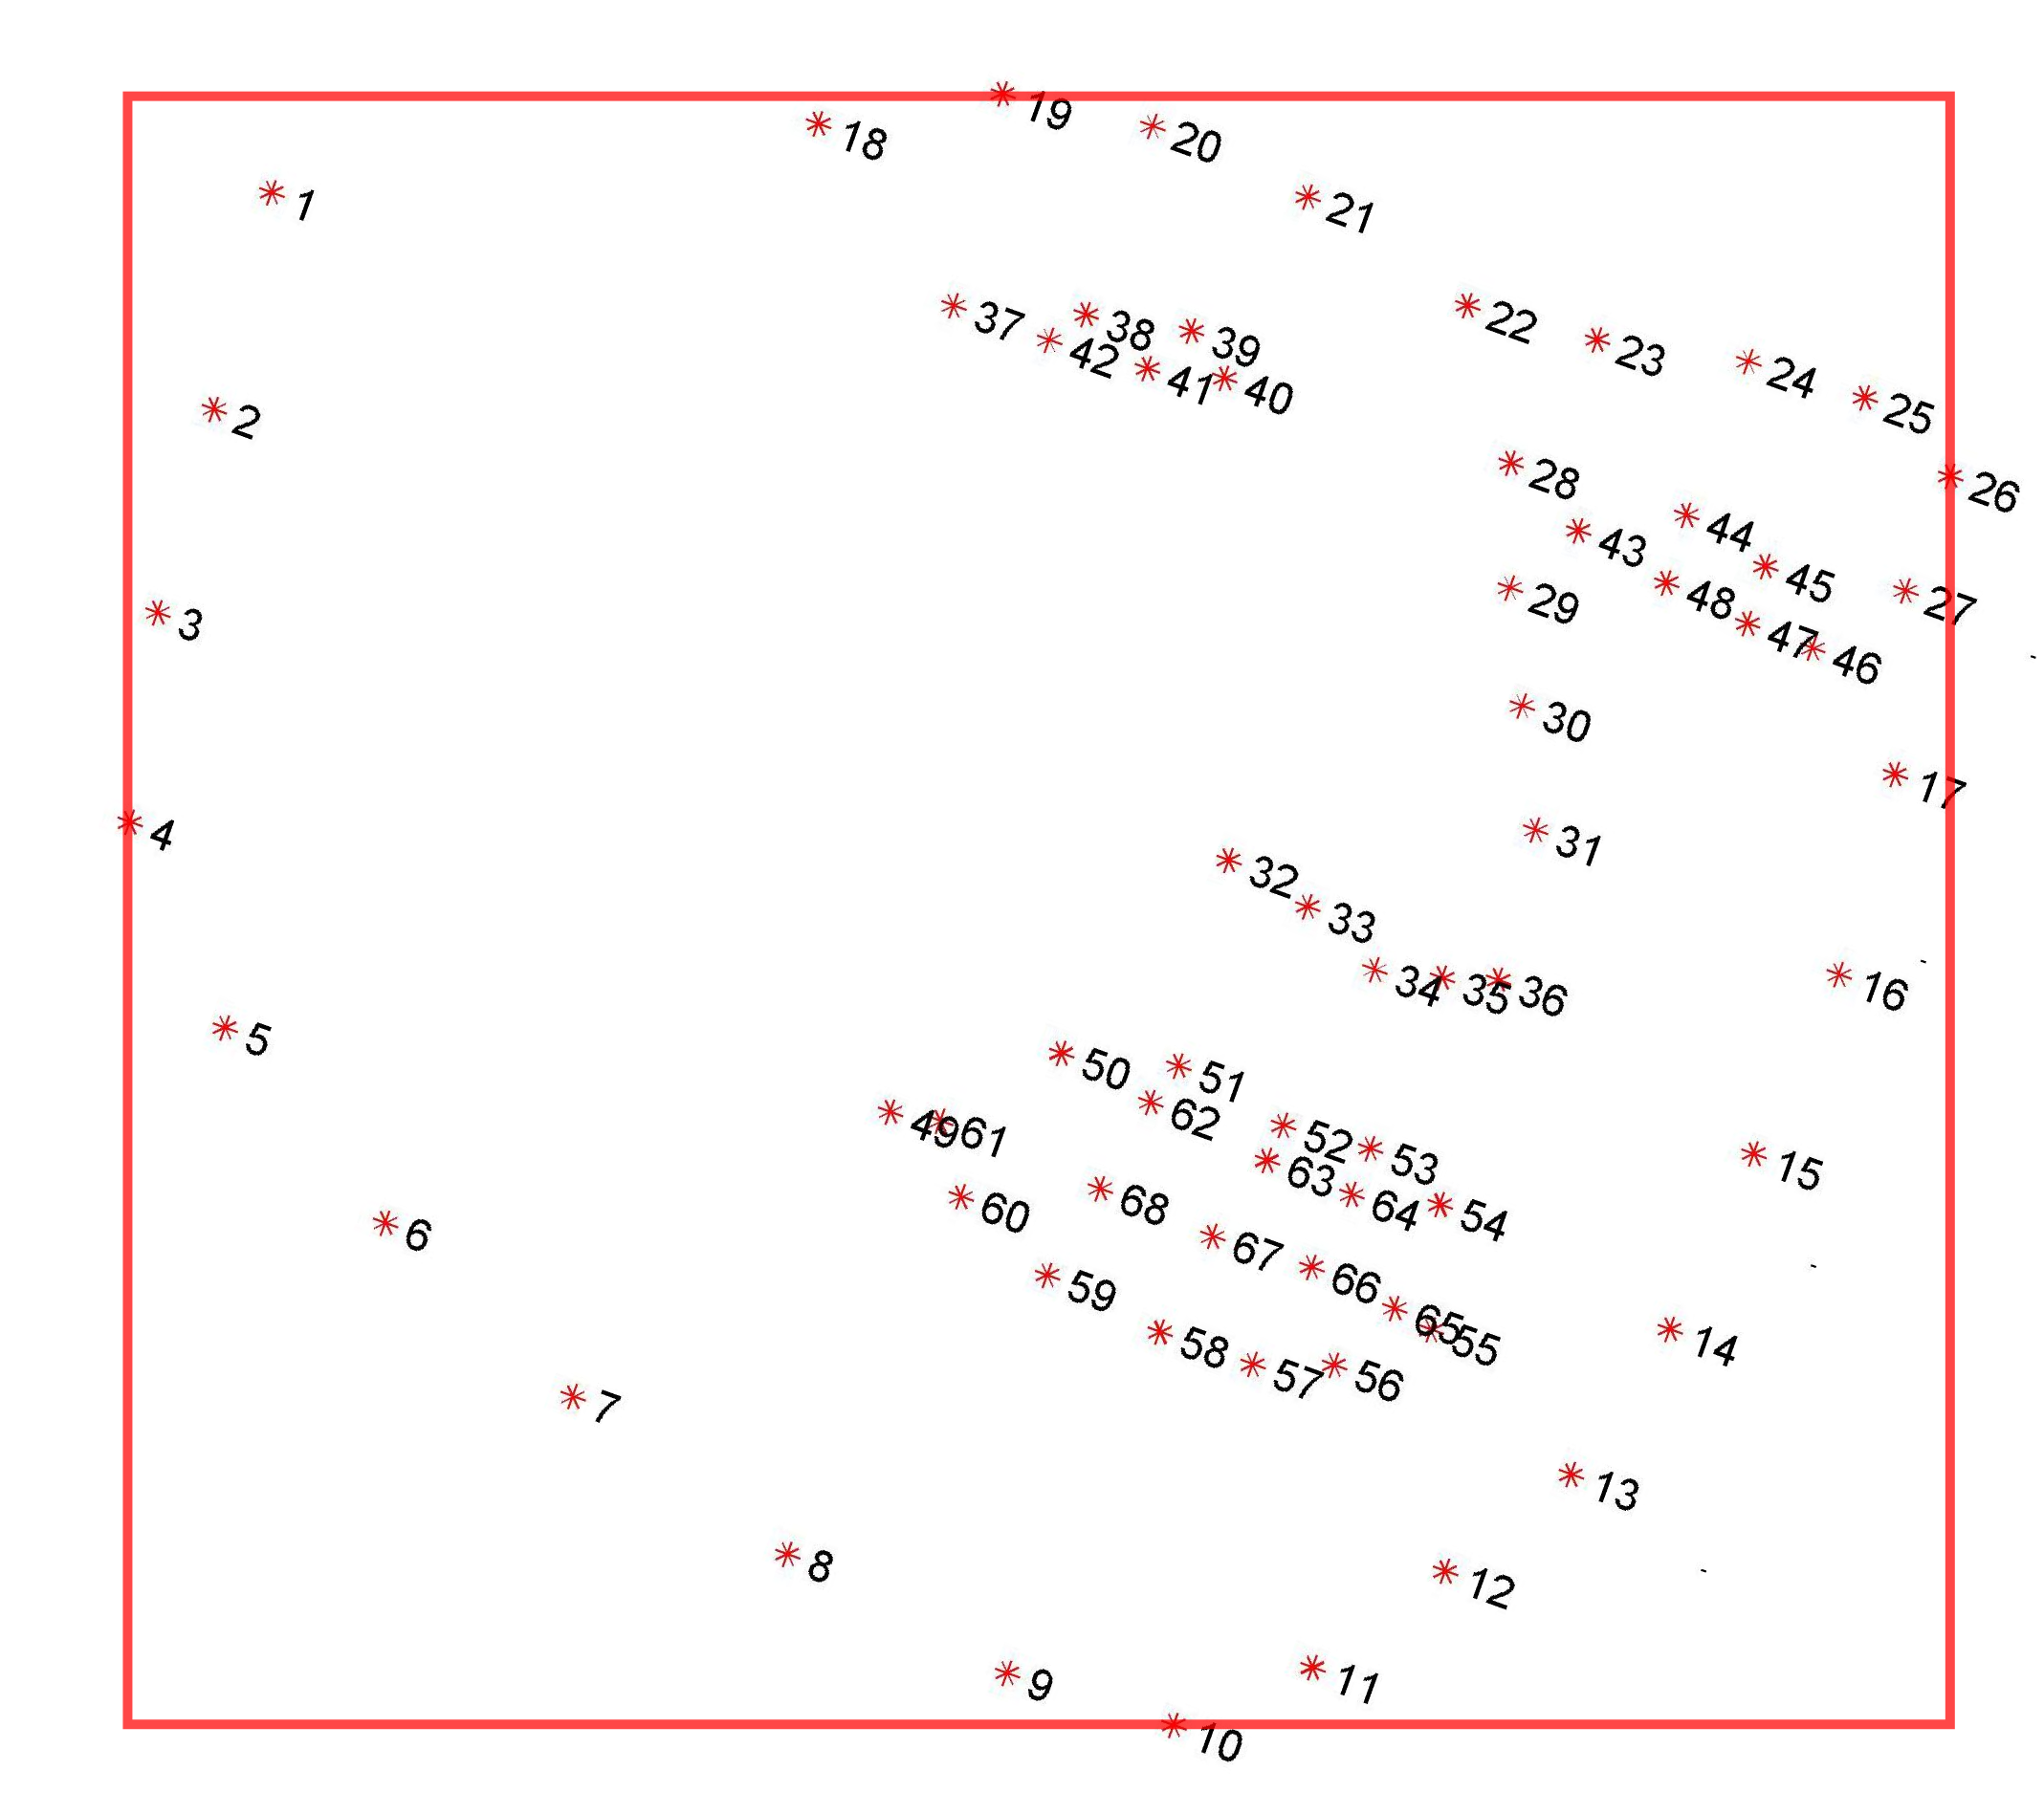
\includegraphics[width=0.49\textwidth]{facial_landmarks_2.png}
    \caption{Repere faciale. Imagini preluate de aici: \url{https://ibug.doc.ic.ac.uk/resources/300-W/}}
    \label{figure:facial-landmarks}
\end{figure}

Folosind anumiți algoritmi deja existenți am detectat aceste puncte faciale din imagini ale utilizatorului aplicației (în acest caz, imagini cu mine însumi) iar apoi am extras regiuni dreptunghiulare care conțineau fie întreaga față, fie ochii persoanei.
Apoi am etichetat aceste imagini decupate cu coordonatele punctelor de pe ecran pe care le privea utilizatorul în fiecare imagine și am dezvoltat un model matematic care poate calcula zona ecranului pe care o privește utilizatorul.

Mai departe am făcut uz de restul reperelor faciale pentru a putea atinge obiectivele prezentate mai devreme.
Fiind capabilă să urmărească ochii, aplicația trebuie și să poată deplasa cursorul, dar într-un mod controlat, care să nu deranjeze privirea normală a ecranului.
Astfel, deplasarea cursorului se realizează doar în momentul în care distanța dintre buza superioară și cea inferioară este nenulă și reprezintă un anumit procent din distanța dintre extremitățile buzelor (care coincid).
În termeni mai populari și mai simpli, relația se traduce prin gestul de deschidere a gurii.

Pentru apăsarea butoanelor am avut o abordare similară.
Prin închiderea ochiului stâng pentru o anumită perioadă de timp se realizează apăsarea butonului stâng.
Analog, apăsarea butonului drept se realizează similar.

\section*{Structura lucrării}
\addcontentsline{toc}{section}{Structura lucrării}
În primul capitol\ref{chapter1} am prezentat principala problemă pe care o analizează această lucrare, și anume urmărirea ochilor (\emph{eye tracking}).
Este prezentată de asemenea strategia pe care am abordat-o spre rezolvarea acestei probleme.

Următorul capitol\ref{chapter2} prezintă soluția propusă împreună cu limitele și constrângerile acesteia.
Am ilustrat structura acesteia, componentele principale și șablonul arhitectural (\emph{design pattern}) folosit pentru a ghida dezvoltarea aplicației.

Capitolele 3\ref{chapter3}, 4\ref{chapter4} și 5\ref{chapter5} urmăresc pașii luați în rezolvarea unei probleme de învățare automată.
Am început cu modul în care am obținut datele de antrenament, modul în care le-am procesat iar apoi am continuat cu prezentarea modului de antrenare și de dezvoltare a arhitecturilor de învățare profundă pe care le-am folosit.
Capitolul 5 prezintă modul în care am folosit predicțiile de urmărire a ochilor în combinație cu repere faciale pentru a simula funcționalitatea unui mouse.

În cele din urmă, capitolul 6\ref{chapter6} ilustrează un experiment pe care l-am făcut pentru identificarea reperelor faciale.
Acesta m-a ajutat la o înțelegere mai bună a modului în care reperele faciale sunt identificate.


    \chapter*{Contribuții} 
\addcontentsline{toc}{chapter}{Contribuții}

Analizând produsele deja existente bazate pe o idee similară am constatat că fiecare dintre ele prezintă un neajuns.
Multe aplicații sunt concepute, spre exemplu, doar pentru sistemul de operare Windows.
O analiză a cotei de piață pentru sistemele de operare pentru sisteme desktop ne indică faptul că există un număr semnificativ de utilizatori care nu folosesc mașini ce rulează Windows.
Așadar, aplicația propusă este \emph{cross-platform}, putând fi rulată pe cele mai importante 3 sisteme de operare: Windows, MacOS și Linux.

\begin{figure}[h]
    \centering
    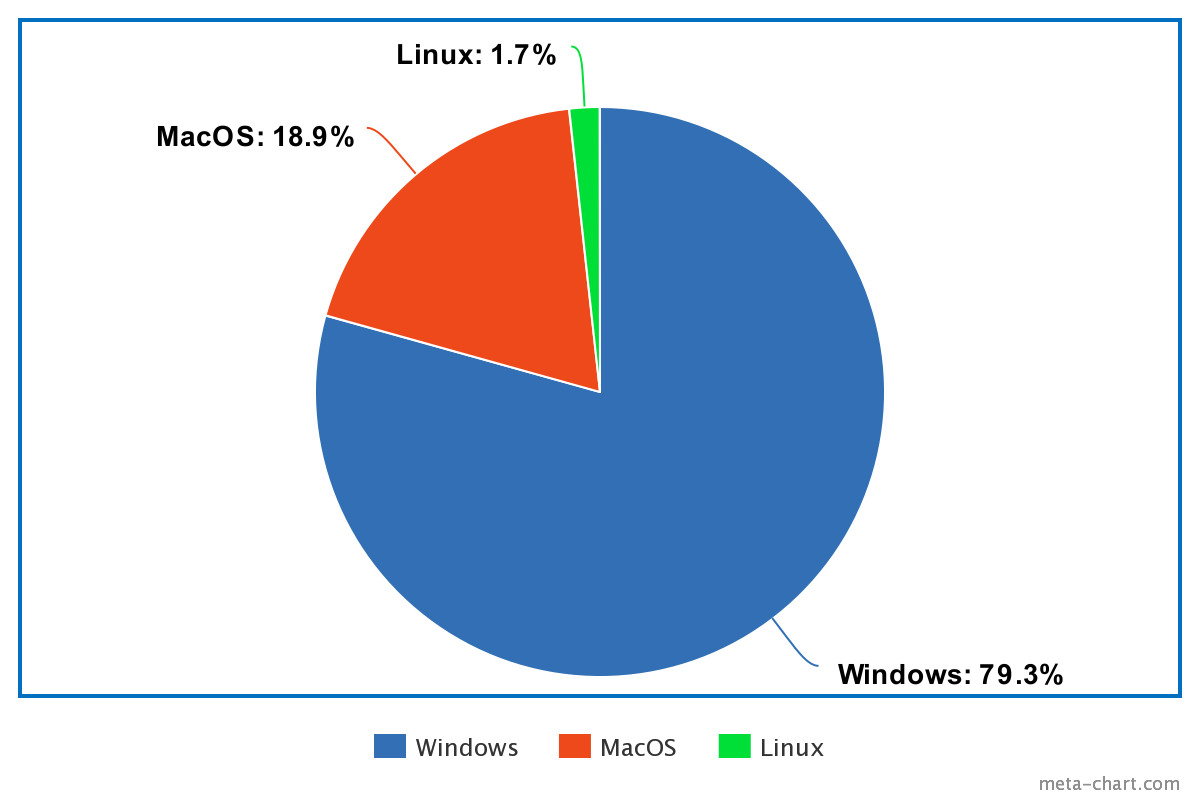
\includegraphics[width=\textwidth]{os.png}
    \caption{Distribuție a sistemelor de operare desktop în Mai, 2020. Date preluate de pe \href{https://gs.statcounter.com/os-market-share/desktop/worldwide}{StatCounter GlobalStats}}
\end{figure}

Un alt punct important este că unele aplicații necesită camere speciale sau senzori speciali, ceea ce aduce un cost în plus și poate fi un impediment în utilizarea aplicației.
Lucrarea de față nu necesită decât o cameră webcam, hardware care este deja existent pe orice laptop comercializat astăzi sau care poate fi atașat unui calculator obișnuit pentru un cost redus.

O ultimă mențiune este legată de diferențele fizionomice dintre persoane.
În acest sens, aplicația se poate ``adapta'' fizionomiei fiecărui utilizator, întrucât pentru a analiza punctul de privire al utilizatorului sunt folosite imagini cu acesta.
Acest lucru aduce un pas în plus pentru ``configurarea'' aplicației (colectarea de date), dar va rezulta într-o experiență mai robustă pentru fiecare utilizator în parte.
    
    \chapter{Prezentarea problemei}
\label{chapter1}
\section{Urmărirea ochilor}
Problema pe care am încercat să o rezolv constă în primul rând în a urmări cu acuratețe ochii utilizatorului, astfel încât cursorul să poată fi mișcat în concordanță cu privirea acestuia.
Această problemă face parte dintr-o gamă mai largă de probleme de \emph{Viziune Computerizată} (în engleză \emph{Computer Vision}), denumită chiar \emph{urmărirea ochilor}, după cum a fost menționat și în introducere.
Conform \cite{eye_tracking}, urmărirea ochilor este ``procesul de măsurare a punctului de privire (unde se uită o persoană) sau a mișcării unui ochi relativ la cap''.\footnote{Textul original este din engleză: ``the process of measuring either the point of gaze (where one is looking) or the motion of an eye relative to the head''}

Tehnicile de ultimă oră (\emph{state of the art}) de a rezolva această problemă se bazează pe \emph{Inteligența Artificială} și sunt, mai exact, tehnici de \emph{Învățare Automată}.
\cite{liviu_ciortuz_ml} explică în termeni foarte simpli acest subdomeniu al informaticii: ``Învățarea Automată este programare bazată pe date''\footnote{Traducere liberă; text original: ``ML is data-driven programming''}.
Învățarea poate fi la rândul ei supervizată, semi-supervizată sau nesupervizată, aceste tehnici încearcând să prezică, să producă, să generalizeze niște rezultate pe baza unor exemple sau a unor relații dintr-o mulțime de date deja cunoscută.
Diferența cheie între acestea constă în structura acestei mulțimi de date, structură care la rândul ei influențează abordările de învățare.

Această ramură a Inteligenței Artificiale poate fi mai departe divizată în mai multe secțiuni, una dintre ele fiind \emph{Invățarea Profundă}.
Ea se preocupă, printre altele, de procesarea și analizarea imaginilor prin folosirea unor \emph{arhitecturi profunde} bazate pe \emph{rețele neuronale}.

Am formulat problema ca una de învățare profundă supervizată, care presupune cunoașterea unei mulțimi de date
$$D = \{(i, o) | i \in I, o \in O\}$$
unde $(i, o)$ reprezină un exemplu, o asociere între un tip de date și un rezultat pe care vrem să îl prezicem, să îl reconstruim.
Pentru fiecare element din mulțimea $I$, avem un element asociat în $O$ care reprezintă mulțimea \emph{adevărurilor de bază} deja cunoscute, pe care trebuie să le putem reproduce și prezice corect pentru alte elemente de tipul celor din mulțimea $I$.

Am definit obiectivul ca fiind acela de a prezice zona de pe ecran pe care o privește utilizatorul.
Pentru acest lucru am plasat o ``grilă'' pe ecran și am numerotat fiecare celulă corespunzătoare.
Am experimentat cu mai multe dimensiuni ale grilei, precum 2x2, 3x2 și 4x4.

\begin{figure}[H]
    \centering
    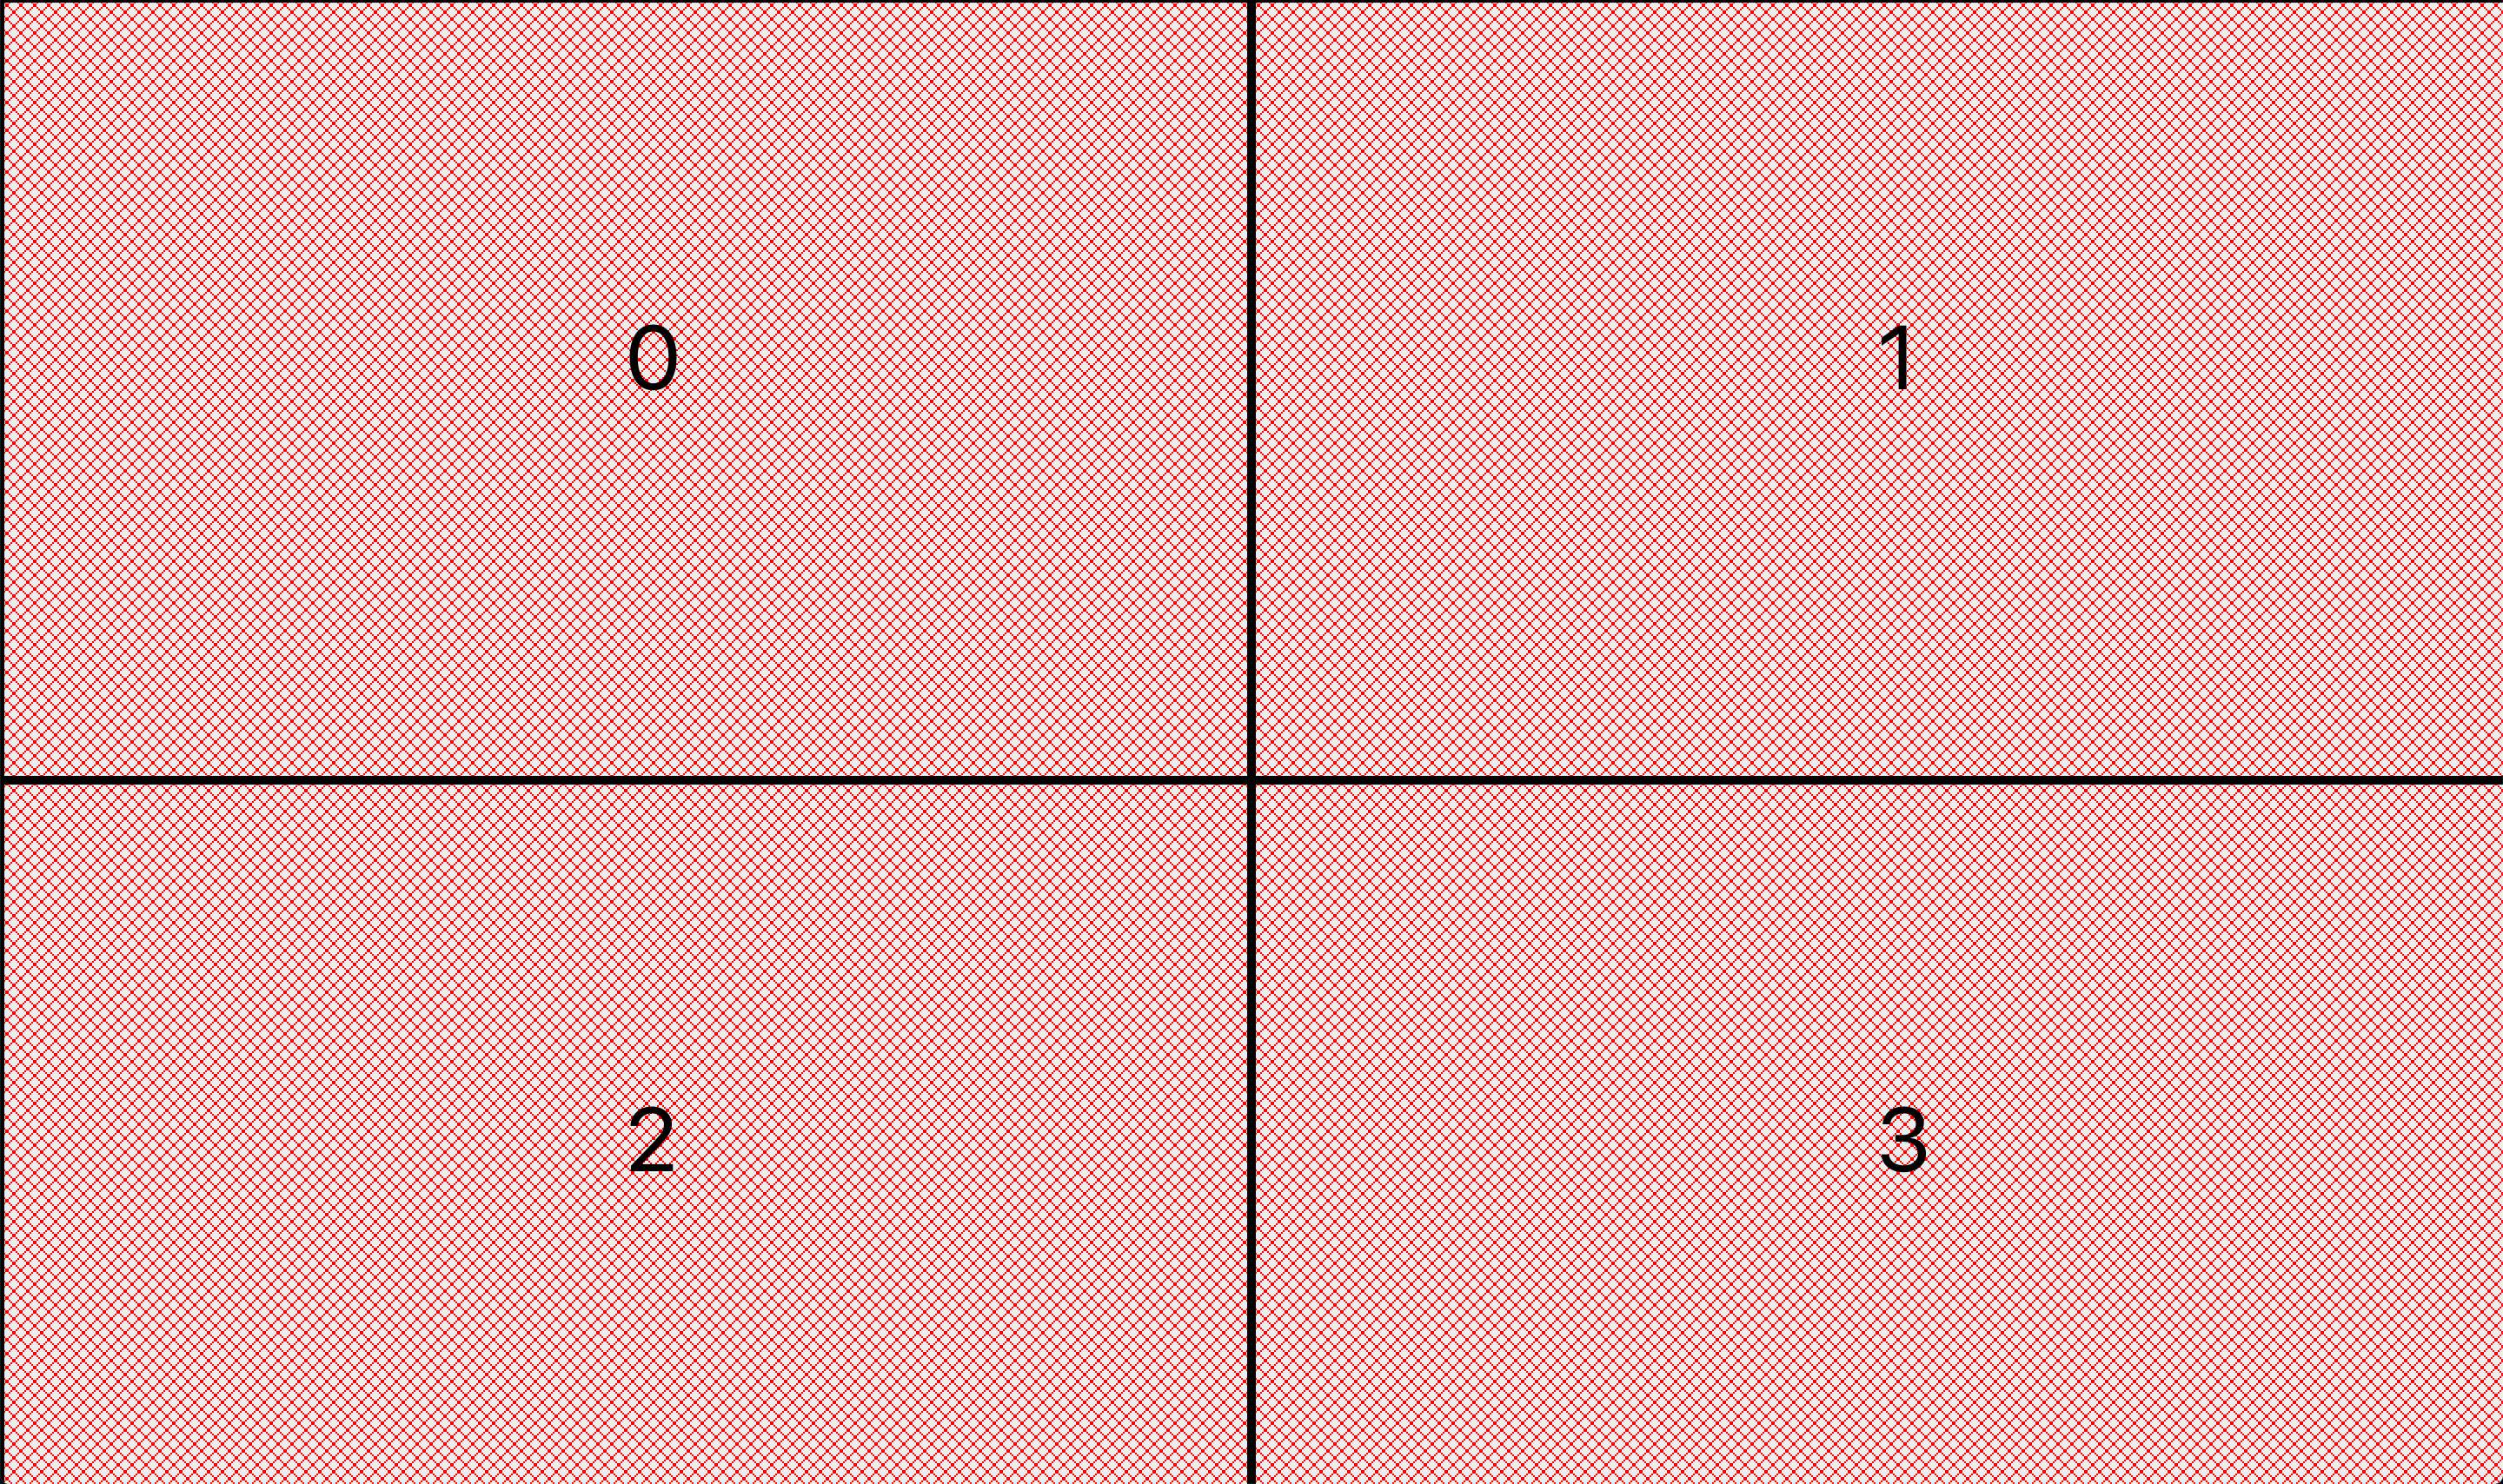
\includegraphics[width=0.32\textwidth]{grid_2_2.png}
    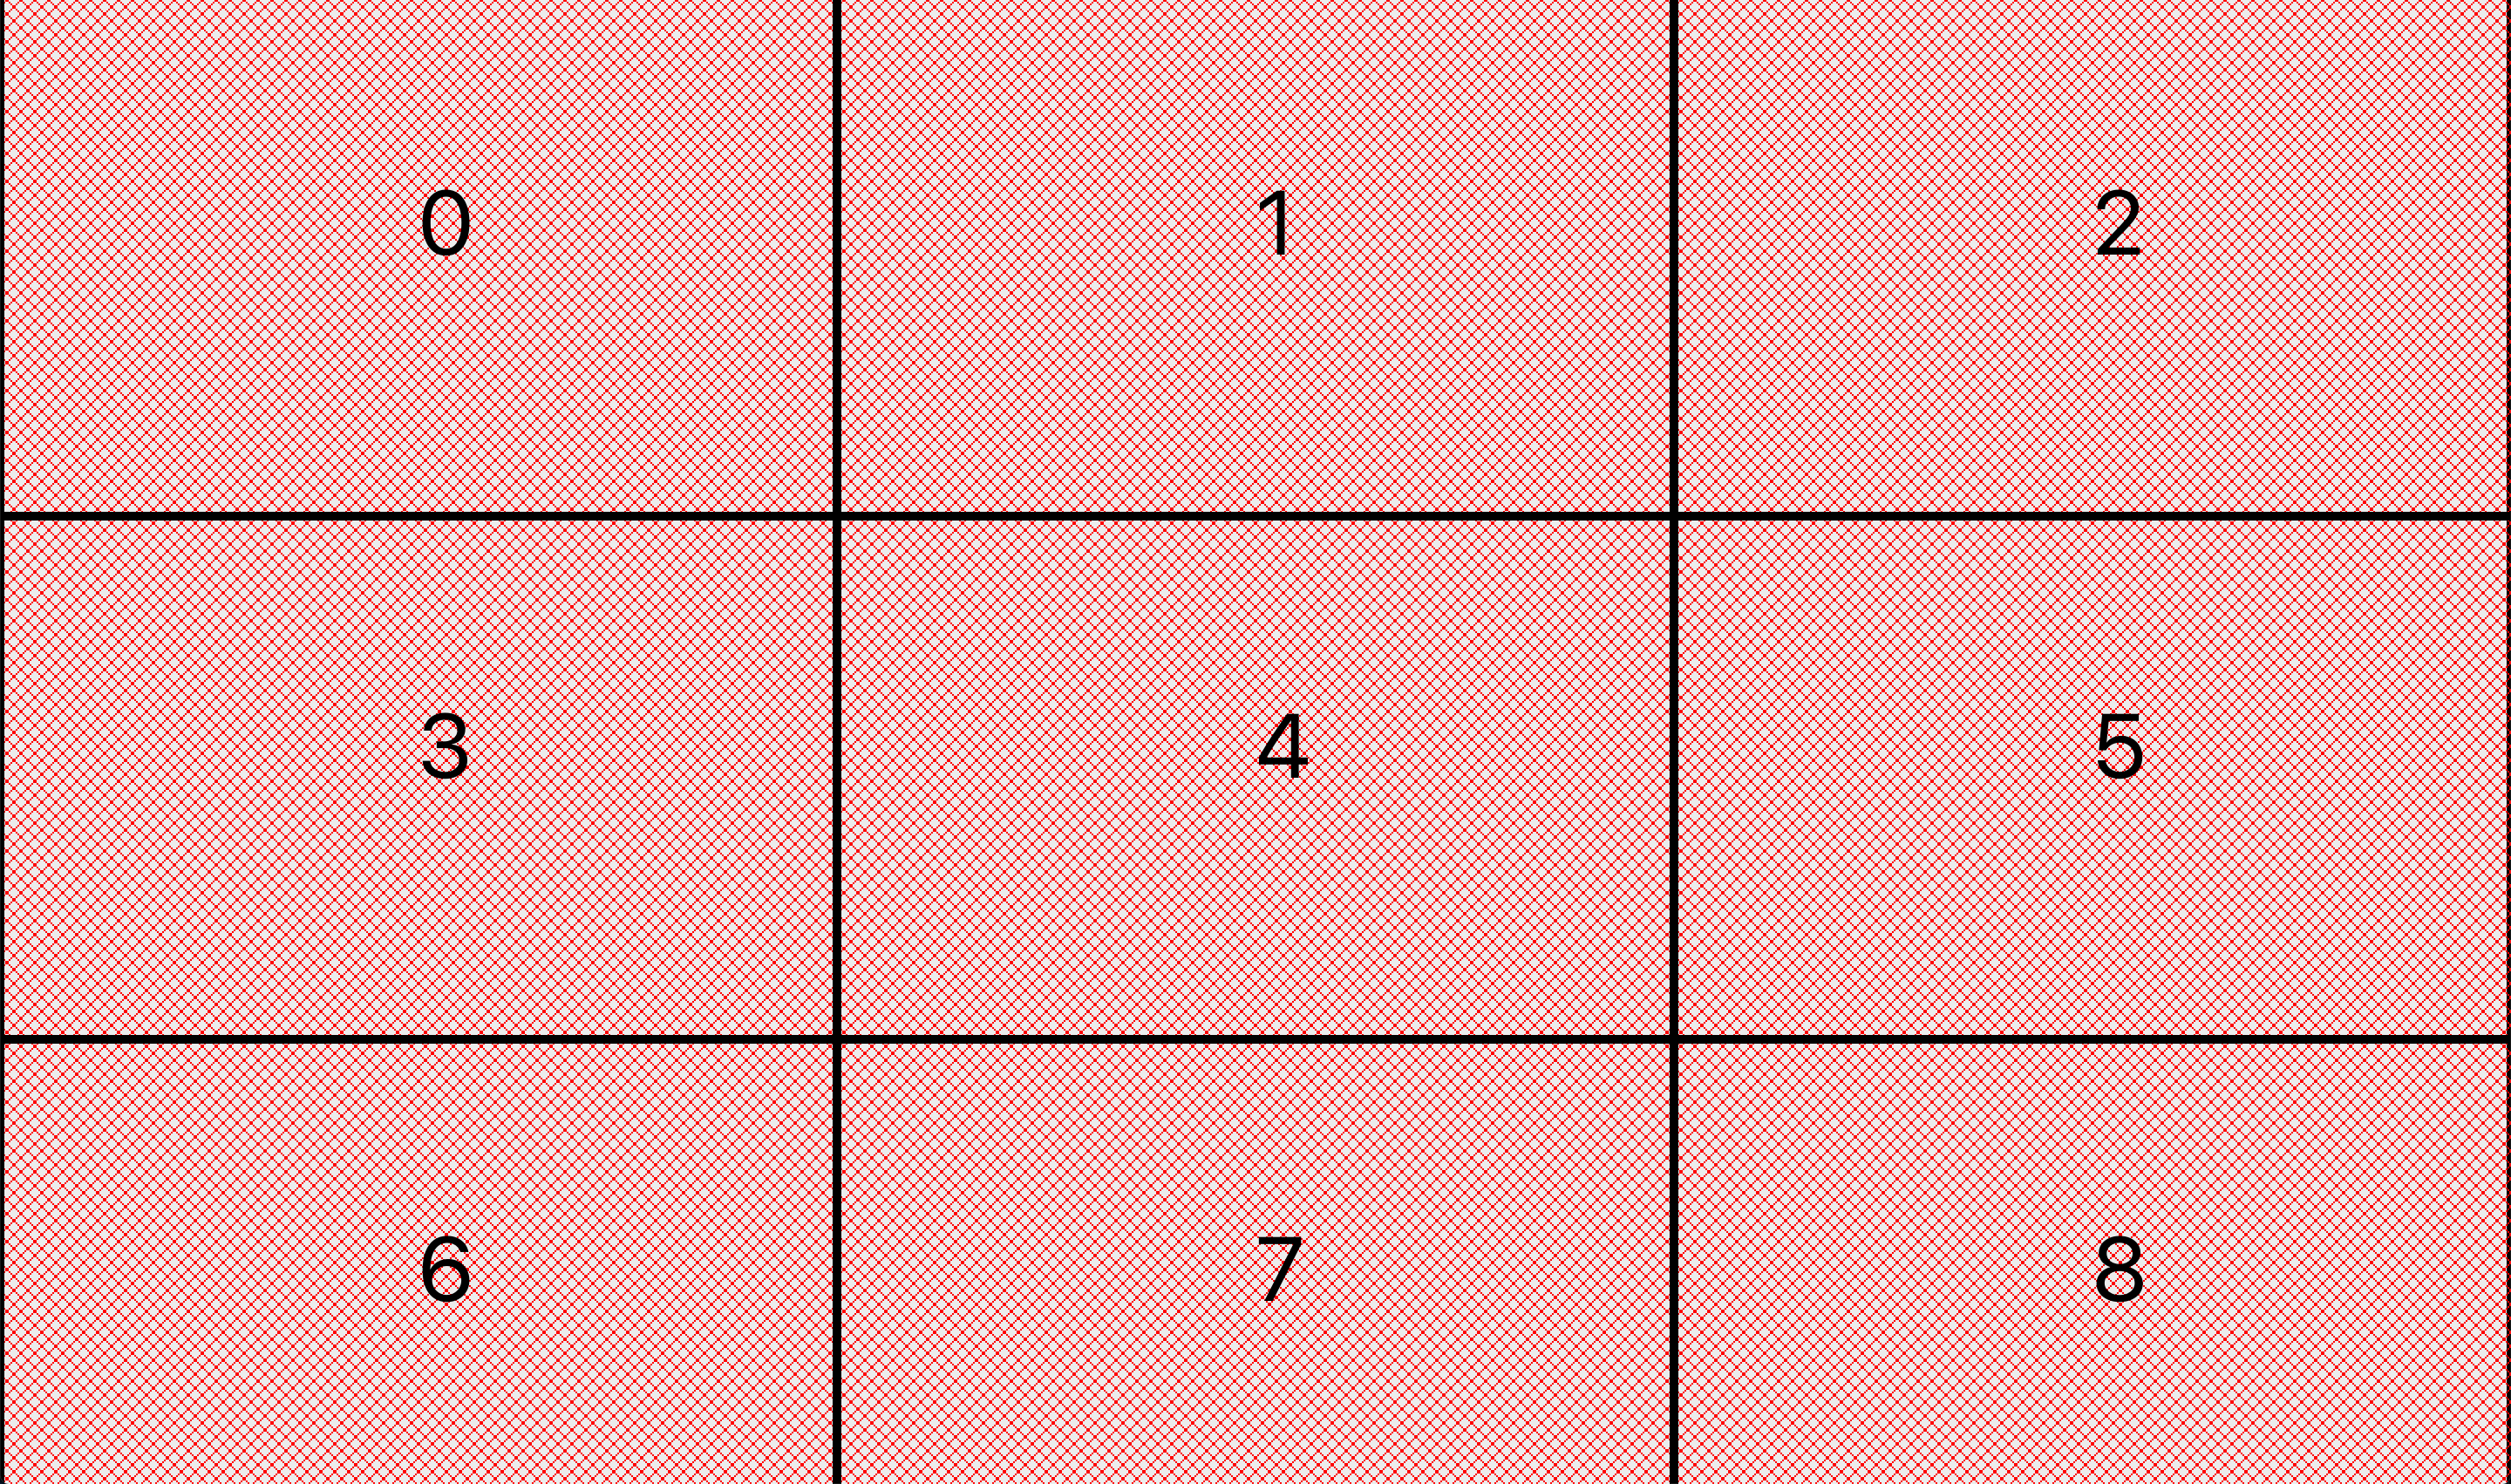
\includegraphics[width=0.32\textwidth]{grid_3_3.png}
    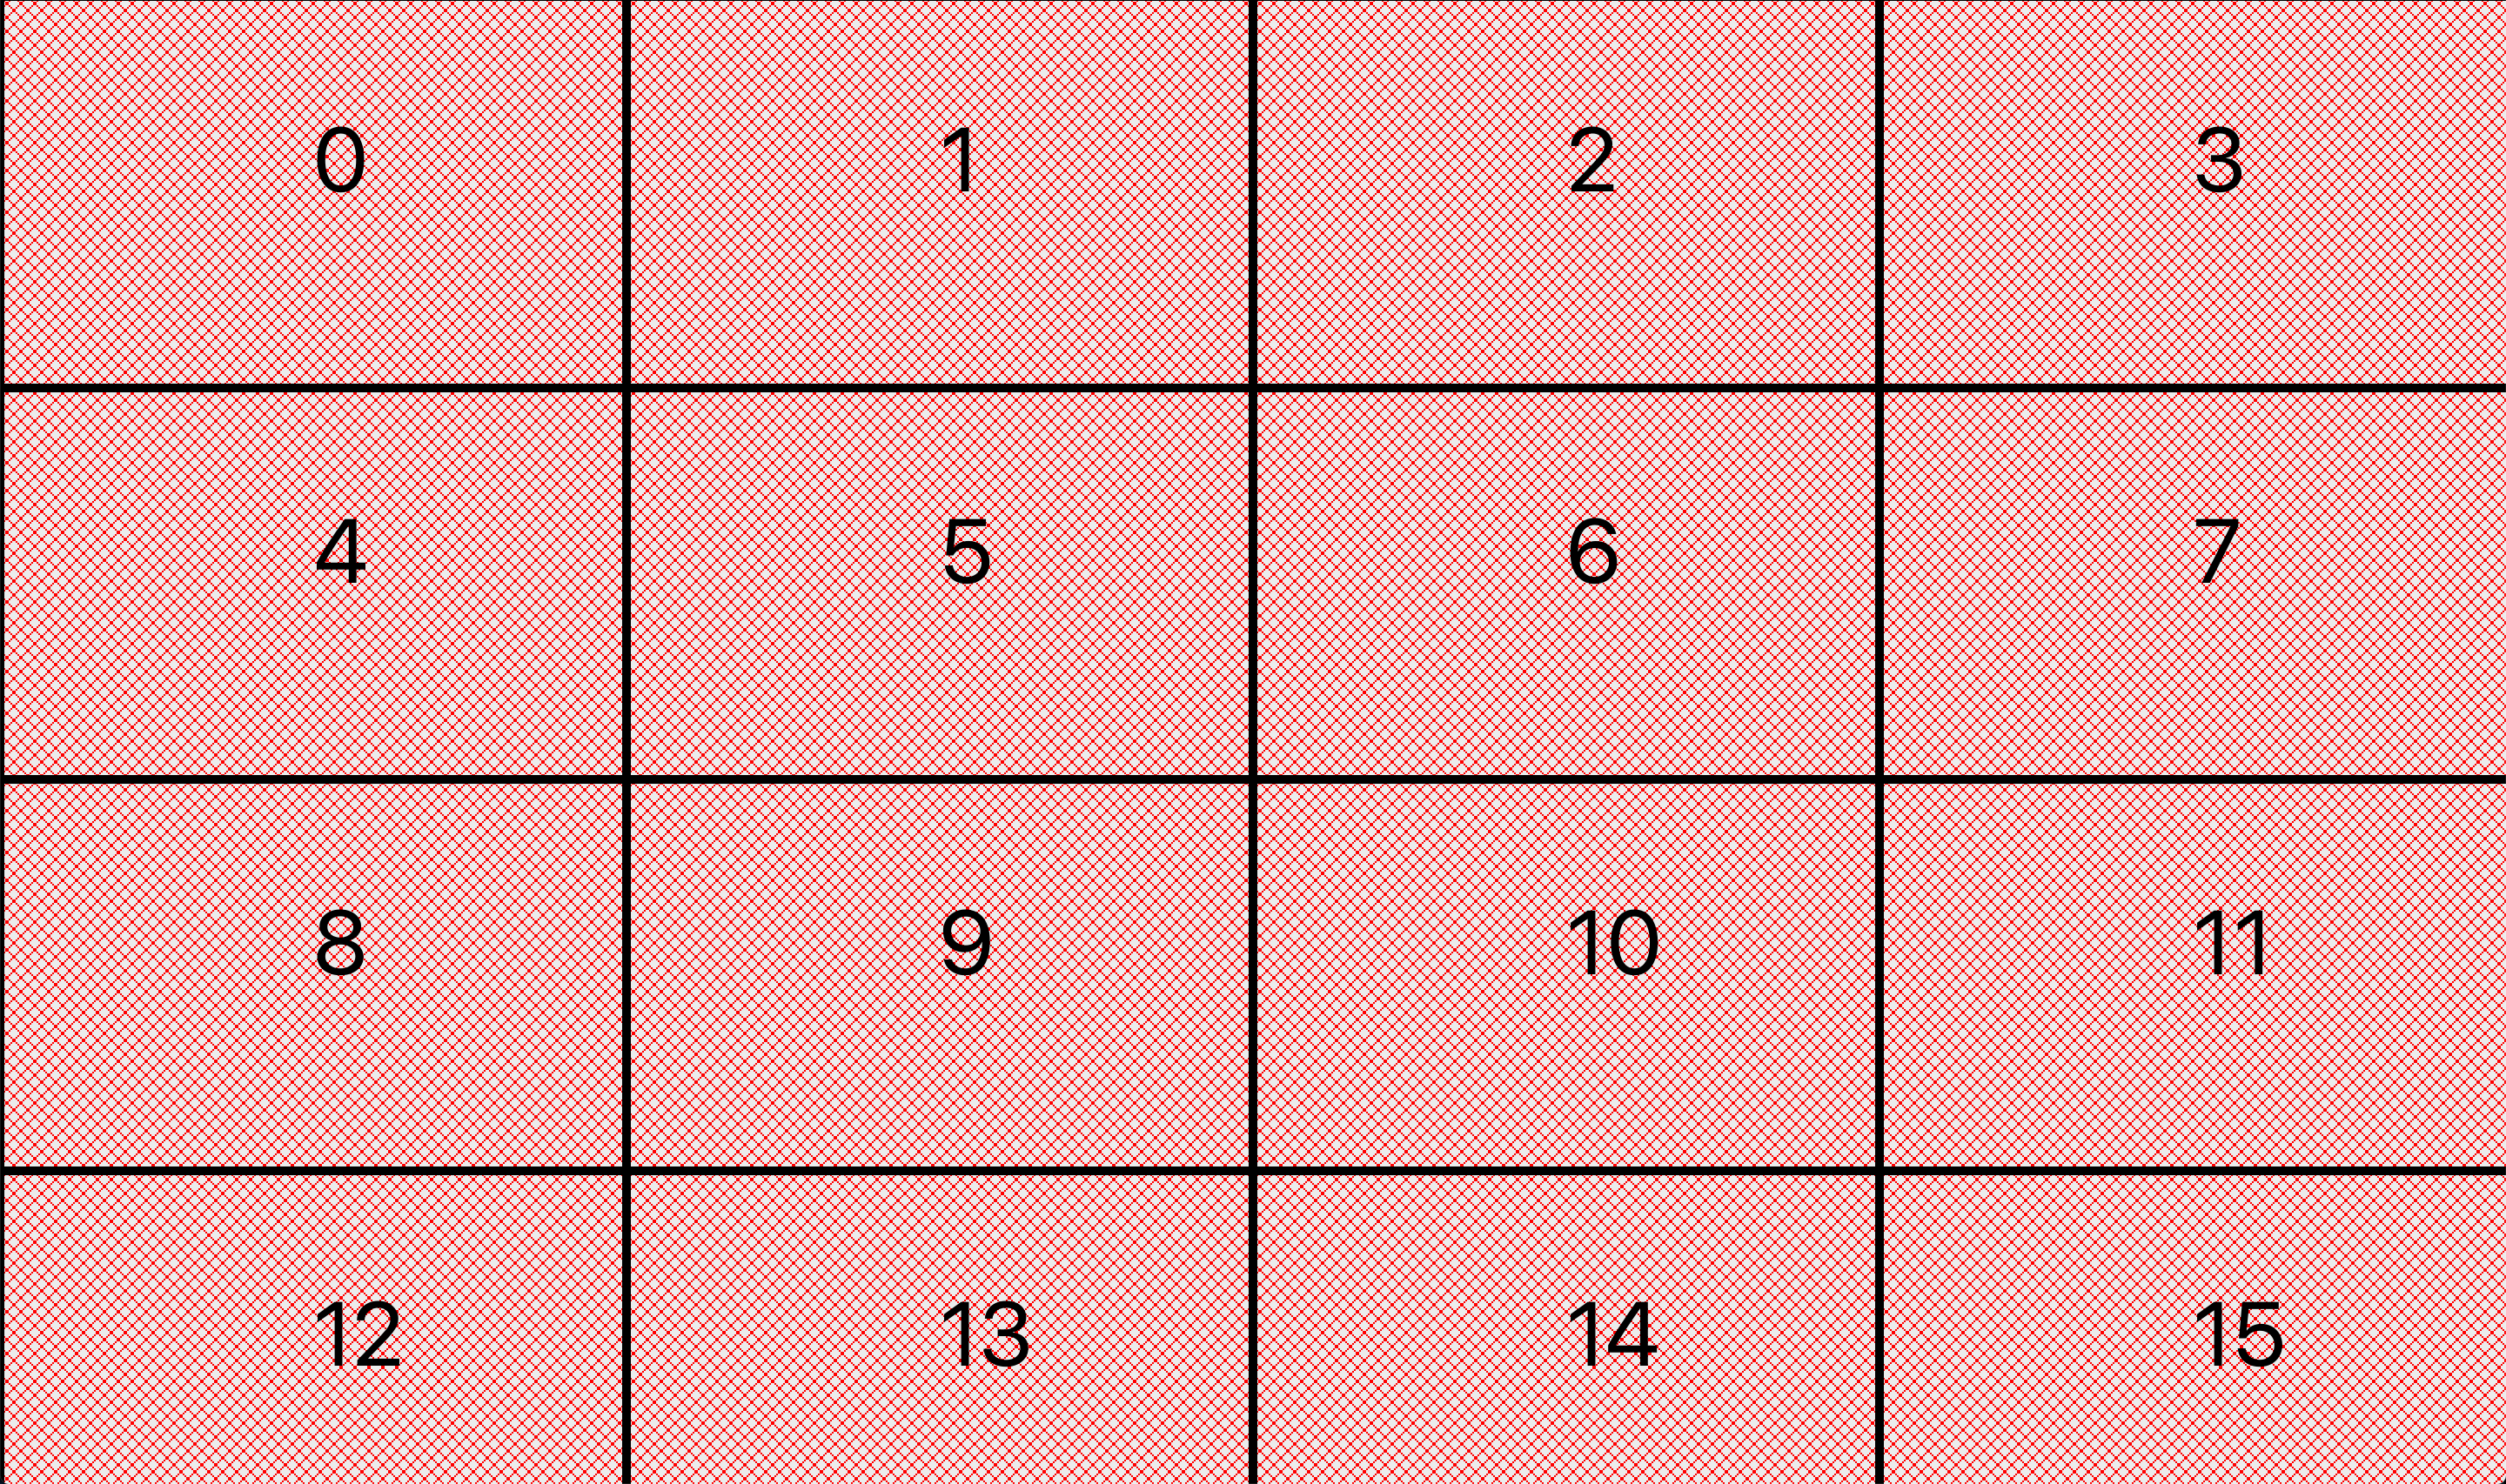
\includegraphics[width=0.32\textwidth]{grid_4_4.png}
    \caption{Exemple de grile plasate pe ecran}
    \label{grid-example}
\end{figure}

Așadar, mulțimea $I$ de mai sus va fi alcătuită din imagini ale utilizatorului, care ar permite ``extragerea privirii'' acestuia, iar mulțimea $O$ va conține, spre exemplu, numărul celulei pe care o privea utilizatorul în imaginea respectivă.
Mulțimea $O$ conține valori discrete și este finită, așadar problema inițială este una de \emph{clasificare}.
Vom considera că mulțimea $I$ nu conține imagini în care utilizatorul nu se uită la un punct de pe ecran.

Prima parte a problemei se traduce, așadar, astfel: dându-se o imagine cu utilizatorul privind ecranul, să se calculeze numărul celulei (în funcție de grila folosită) pe care utilizatorul o privește.

\section{Simularea funcționalităților mouse-ului}
A doua parte a problemei ridică următoarea întrebare: cum putem simula un mouse folosind reperele faciale?
Cum asigurăm o mișcare fluidă a cursorului spre o ``zonă țintă'', dar în același timp cursorul să poată rămâne fix?
Dacă am deplasa constant cursorul pe ecran, în funcție de punctul de privire, atunci utilizatorul ar putea fi distras atunci când doar ar privi ecranul (de exemplu când ar citi un document) sau ar efectua operația de click stânga/dreapta accidental, asupra altor elemente grafice.

Fiecare zonă a ecranului conține un număr finit de pixeli pe care utilizatorul i-ar putea privi.
Trebuie să-i putem oferi astfel utilizatorului posibilitatea de a deplasa cursorul asupra acestor pixeli.
Un buton plasat pe câțiva pixeli ar fi aproape imposibil de apăsat pe orice ecran digital contemporan și ar și obosi ochii, așa că orice element grafic al unei aplicații software se întinde pe un număr mai mare de pixeli.
Profitând de acest lucru, putem spune că aplicația trebuie să poată deplasa cursorul \emph{aproape} de orice pixel al ecranului.

În cele din urmă mai rămâne doar simularea apăsării butoanelor de pe mouse.
Utilizatorul trebuie să poată solicita într-un mod explicit acest lucru, folosindu-se doar de față, iar aplicația trebuie să asigure evitarea cazurilor de tipul \emph{false positive}, adică a apăsărilor butoanelor atunci când acest lucru nu este dorit.

% \subsection{Neuronul Artificial}

% Înainte de a analiza arhitecturi de învățare profundă mai sofisticate, trebuie să aruncăm o privire rapidă asupra neuronului artificial.
% Pe scurt, este un model formal, simplificat al unui neuron biologic.
% Ne poate ajuta să realizăm \emph{clasificare binară} folosind următoarea formulă:
% $$
% y = \varphi (w * x + b)
% $$

% În formula de mai sus, $x$ este un vector de valori reale, reprezentând datele de intrare, iar $w$ este un vector de valori reale denumit \emph{vectorul ponderilor} (în engleză \emph{weights}) și $b$ este \emph{parțialitatea} (în engleză \emph{bias-ul}).
% Produsul $w * x$ reprezintă produsul scalar și este egal cu $w * x = \sum _{i=1}^{n}w_{i}x_{i}$, $n$ fiind lungimea vectorului $x$.


% Rezultatul clasificării este dat de $\varphi$, denumit \emph{funcție de activare}.
% Daca aceasta se comportă ca un prag, o limită, un \emph{threshold}, atunci funcția de activare se va traduce într-o clasificare binară, cu rezultat $0$ sau $1$.
% Putem folosi și $\varphi(x) = x$, ecuație care ne poate ajuta la rezolvarea problemelor de tip \emph{regresie liniară}.

% \begin{figure}[h]
%     \centering
%     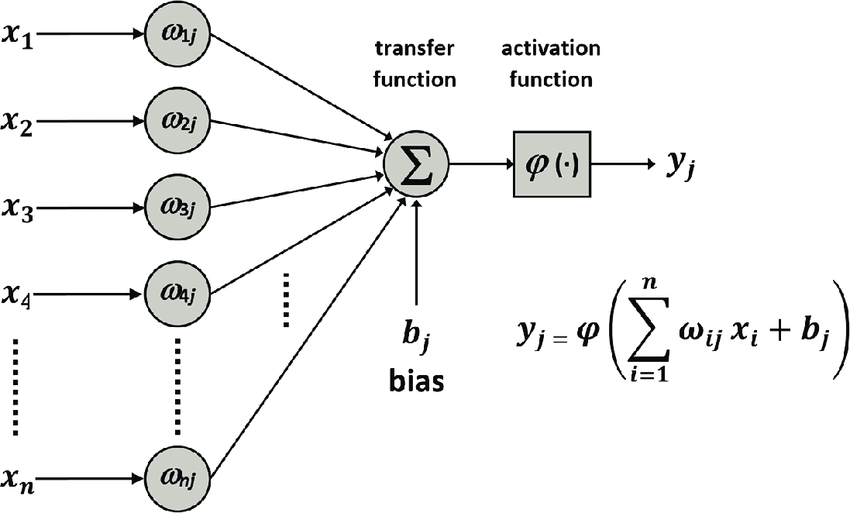
\includegraphics[width=\textwidth]{artificial_neuron.png}
%     \caption{Algoritmul perceptron, bazat pe neuronul artificial. Imagine preluată de pe site-ul \href{https://www.researchgate.net/figure/Scheme-of-a-perceptron-A-nonlinear-activation-function-BULLET-is-applied-to-the_fig3_315788933}{ResearchGate}}
% \end{figure}


% \subsection{Rețele neuronale}

% ``Calul de bătaie'' pentru problemele de Viziune Computerizată este Rețeaua Neuronală Artificială.
% Ea este, dupa cum sugerează și numele, compusă din mai multi neuroni artificiali, distribuiți pe mai multe \emph{straturi}.

% \begin{figure}[H]
%     \centering
%     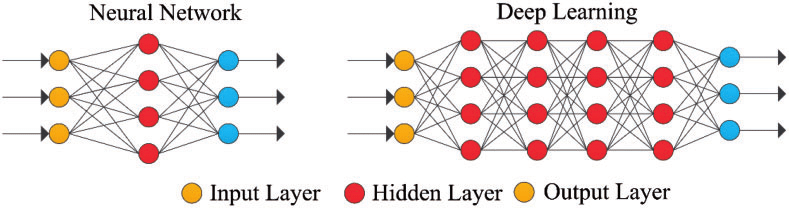
\includegraphics[width=\textwidth]{ann.png}
%     \caption{Structură generală a unei rețele neuronale. Imagine preluată de pe site-ul \href{https://www.researchgate.net/figure/Deep-learning-diagram_fig5_323784695}{ResearchGate}}
% \end{figure}

\section{Strategie}

\subsection{Obținerea datelor de antrenament}
Primul pas spre rezolvarea problemei este \emph{colectarea datelor de antrenament}.
Este foarte bine cunoscut că un algoritm de învățare automată este pe atât de bun pe cât sunt datele pe care i le furnizăm.
Acestea sunt incredibil de importante, așa că m-am concentrat pe a dezvolta niște modalități facile de a aduna o mulțime consistentă de date.

O altă etapă esențială este \emph{procesarea de date}.
Aceasta se preocupă cu simplificarea și curățarea setului de date, cu eliminarea instanțelor de antrenament care sunt inutile și cu extragerea exclusiv a informațiilor care sunt de folos și cu înlăturarea a ceea ce rămâne.
Opțional, în această etapă se mai realizează și diferite transformări pentru a aduce datele dintr-o formă neprelucrată într-o formă convenabilă algoritmilor pe care îi folosim.
În acest sens, am procesat datele neprelucrate în diverse moduri pentru a determina cea mai utilă stare în care le pot aduce.

\subsection{Predicția zonei de privire}
Următorul pas a fost cel de antrenare și de dezvoltare a unui model matematic capabil să prezică zona de privire a utilizatorului.
Pentru acest lucru m-am concentrat pe studiul \emph{rețelei neuronale}, văzută drept ``calul de bătaie'' și baza pentru problemele de Viziune Computerizată.
% Un tip special de rețea neuronală este \emph{Rețeaua Neuronală Artificială} (\emph{Multilayer Perceptron Network}).
% Ea este, dupa cum sugerează și numele, compusă din mai multi neuroni artificiali, distribuiți pe mai multe \emph{straturi}.
Am folosit o arhitectură bazată pe aceasta (rețeaua de tip \emph{MLP}) ca un punct de pornire spre a rezolva problema și ca un prim experiment.

% \begin{figure}[ht]
%     \centering
%     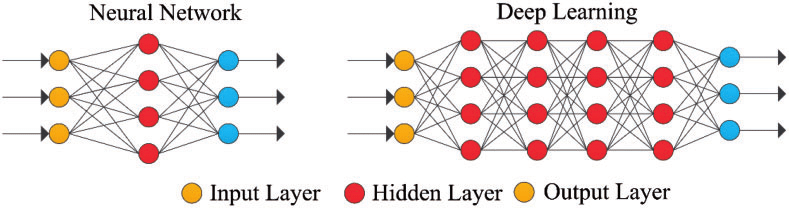
\includegraphics[width=\textwidth]{ann.png}
%     \caption{Structură generală a unei rețele neuronale. Imagine preluată de pe site-ul \href{https://www.researchgate.net/figure/Deep-learning-diagram_fig5_323784695}{ResearchGate}}
% \end{figure}

Folosind acest tip de rețea, am încercat să ating cel mai important obiectiv al acestei lucrări al licenței, și anume de a prezice aproximativ zona în care se uită utilizatorul, pentru a putea deplasa cursorul în acea zonă.
Din experimentele efectuate, această arhitectură a rezultat într-o primă soluție promițătoare, fiind capabilă să urmărească, într-o anumită măsura, privirea utilizatorului.

Apoi a urmat studierea și aplicarea \emph{rețelelor neuronale convoluționale}, o arhitectură de bază pentru multe metode \emph{state of the art} pentru problemele din domeniul Viziunii Computerizate.
Cu ajutorul acestora, urmărirea ochilor a devenit mai robustă și mai puțin sensibilă la diferențele dintre imagini, precum lumină sau poziționarea persoanei în fața webcam-ului.

\subsection{Simularea funcționalităților mouse-ului}
Având un model care poate satisface nevoia de mai sus, de urmărire a ochilor, am analizat apoi cum pot simula efectiv funcționalitatea unui mouse.
Pentru aceasta, am analizat modalități de a folosi reperele faciale\ref{figure:facial-landmarks} pentru a folosi gesturi ale feței și a simula aceste funcționalități.
Soluția a constat în a folosi gesturi precum închiderea unui ochi și gestul de deschidere a gurii.

\subsection{Cercetare și analizare a bibliotecilor folosite}
În lucrarea de licență am folosit diverse biblioteci printre care și \lstinline{dlib}, pe care am folosit-o pentru a identifica reperele faciale ale utilizatorului.
Am fost curios despre cum anume funcționează această bibliotecă și am făcut un mic experiment în care am încercat să reconstruiesc funcționalitatea acestei librării.
    % \chapter{Soluția propusă}
\label{chapter2}
\section{Informații preliminare}
\subsection{Informații tehnice}
Pentru dezvoltarea, structurarea și versionarea codului sursă al lucrării, am folosit platforma gratuită Github\footnote{\url{https://github.com}}.
\emph{Repository-ul} proiectului poate fi accesat la această adresă: \url{https://github.com/sergiuiacob1/iClicker/}.

Rezultatele prezentate aici au fost bazate pe imagini capturate prin intermediul unei camere webcam capabile de o rezoluție maximă HD (1280x720 pixeli).
Experimentele realizate au fost făcute în general în medii bine luminate, întrucât o dată cu scăderea intensității luminii suferă și utilitatea aplicației prezentate aici.

\subsection{Python \& Conda}
Unul dintre cele mai populare limbaje de programare când vine vorba de Învățare Profundă este Python.
Astfel, am ales să dezvolt aplicația folosind acest limbaj, deoarece suportul din partea comunității este unul foarte bun și resursele găsite online pentru a rezolva probleme comune sunt vaste.

Am facut uz de asemenea de tehnologia Conda care ajută în gestionarea mediilor de dezvoltare.
Cu ajutorul acestora am putut crea un mediu de dezvoltare separat, care se poate instala cu ușurință pe orice calculator fără a crea conflicte cu alte pachete deja existente pe mașina unui utilizator.
Această combinație a ajutat la îndeplinirea necesității aplicației de a rula pe mai multe sisteme de operare, întrucât Python deja satisface această nevoie.
Versiunile folosite au fost \lstinline{Python 3.7} și Conda \lstinline{4.8.0}.

\subsection{OpenCV}
Una dintre bibliotecile Python care au adus funcționalități cruciale acestui proiect este OpenCV.
Aceasta conține diferite funcționalități legate de Viziunea Computerizată, precum captura de imagini prin intermediul webcam-ului.
Am folosit-o de asemenea pentru a realiza redimensionări de imagini, pentru a le converti în gri sau în imagini alb-negru prin aplicarea unui \emph{binary threshold}.
Versiunea folosită a fost \lstinline{4.1.2}.

\subsection{PyQt5}
Aplicația dezvoltată are și o interfață grafică ce a fost implementată folosind biblioteca PyQt5.
Unul dintre avantajele acestei biblioteci este acela că oferă un nivel înalt de abstractizare și componentele (butoanele, ferestrele etc.) grafice au un aspect diferit în funcție de sistemul de operare pe care rulează aplicația, fără a fi nevoie ca acest lucru să fie implementat de dezvoltator.
Versiunea folosită a fost \lstinline{5.14}.

\subsection{Keras \& PyTorch}
Keras și PyTorch au fost folosite pentru a facilita antrenarea rețelelor neuronale (de tip \emph{MLP} sau \emph{CNN}).
Acestea au mărit cu mult realizarea arhitecturilor pentru învățarea automată, Keras având un nivel de abstractizare decât PyTorch.
Am folosit cele două tehnologii pentru a căpăta experiență în utilizarea amândurora, întrucât nu există o ``cea mai bună unealtă'', ci mai degrabă contextul nevoii dictează uneltele, tehnologiile ce ar trebui folosite.
Versiunile folosite au fost \lstinline{Keras 2.2.4} și PyTorch \lstinline{1.4}.

\subsection{dlib}
Cea mai importantă bibliotecă de care am făcut uz în această lucrare este dlib.
Cu ajutorul acesteia, am putut realiza identificarea reperelor faciale într-o imagine care conținea fața unei persoane.
Reperele respective sunt furnizate de către sub forma unei liste de coordonate $(x, y)$ corespunzătoare pixelilor acelor caracteristici faciale.
Mai departe, pe baza acestora, am putut decupa fie fața, fie ochii persoanei în imagini mai mici pe care le-am folosit mai apoi ca date de antrenament.
Versiunea folosită a fost \lstinline{19.19.0}.

\section{Limite și constrângeri}
Aplicația are niște limite și lucrează de asemenea cu niște presupuneri, precum faptul că utilizatorul folosește un singur monitor și un singur webcam.
De asemenea, imaginile folosite sunt cu mine însumi, deci trebuie luat acest lucru pentru orice rezultat prezentat.

Aplicația este menită să se poată ``mula'' pe fizionomia utilizatorului, însă este posibil să aibă performanțe mai slabe pentru persoanele care poartă ochelari.
Motivul pentru care se întâmplă acest lucru este acela că aplicația lucrează cu ochii utilizatorului, iar dacă lumina se reflectă în lentilele ochelarilor, ochii ar putea fi indistinctibili.
Ca o ultimă mențiune, aplicația se concentrează majoritar pe poziția pupilelor relativ la ochi (glob ocular + anexe ale globului ocular), deci se va considera că poziția capului nu va suferi schimbări majore între datele de antrenament și datele de test.

\section{Structura aplicației}
Aplicația are 4 mari componente, corespunzătoare pașilor luați în rezolvarea unei probleme de învățarea automată: colectarea de date, procesarea acestora, antrenarea unei rețele convoluționale care realizează urmărirea ochilor și simularea funcționalităților mouse-ului.
Utilizatorul poate interacționa cu aceste componente prin intermediul interfaței grafice realizată în PyQt5.
Fereastra principală a aplicației are și o parte în care vor fi afișate informații utile.

\begin{figure}[ht]
    \centering
    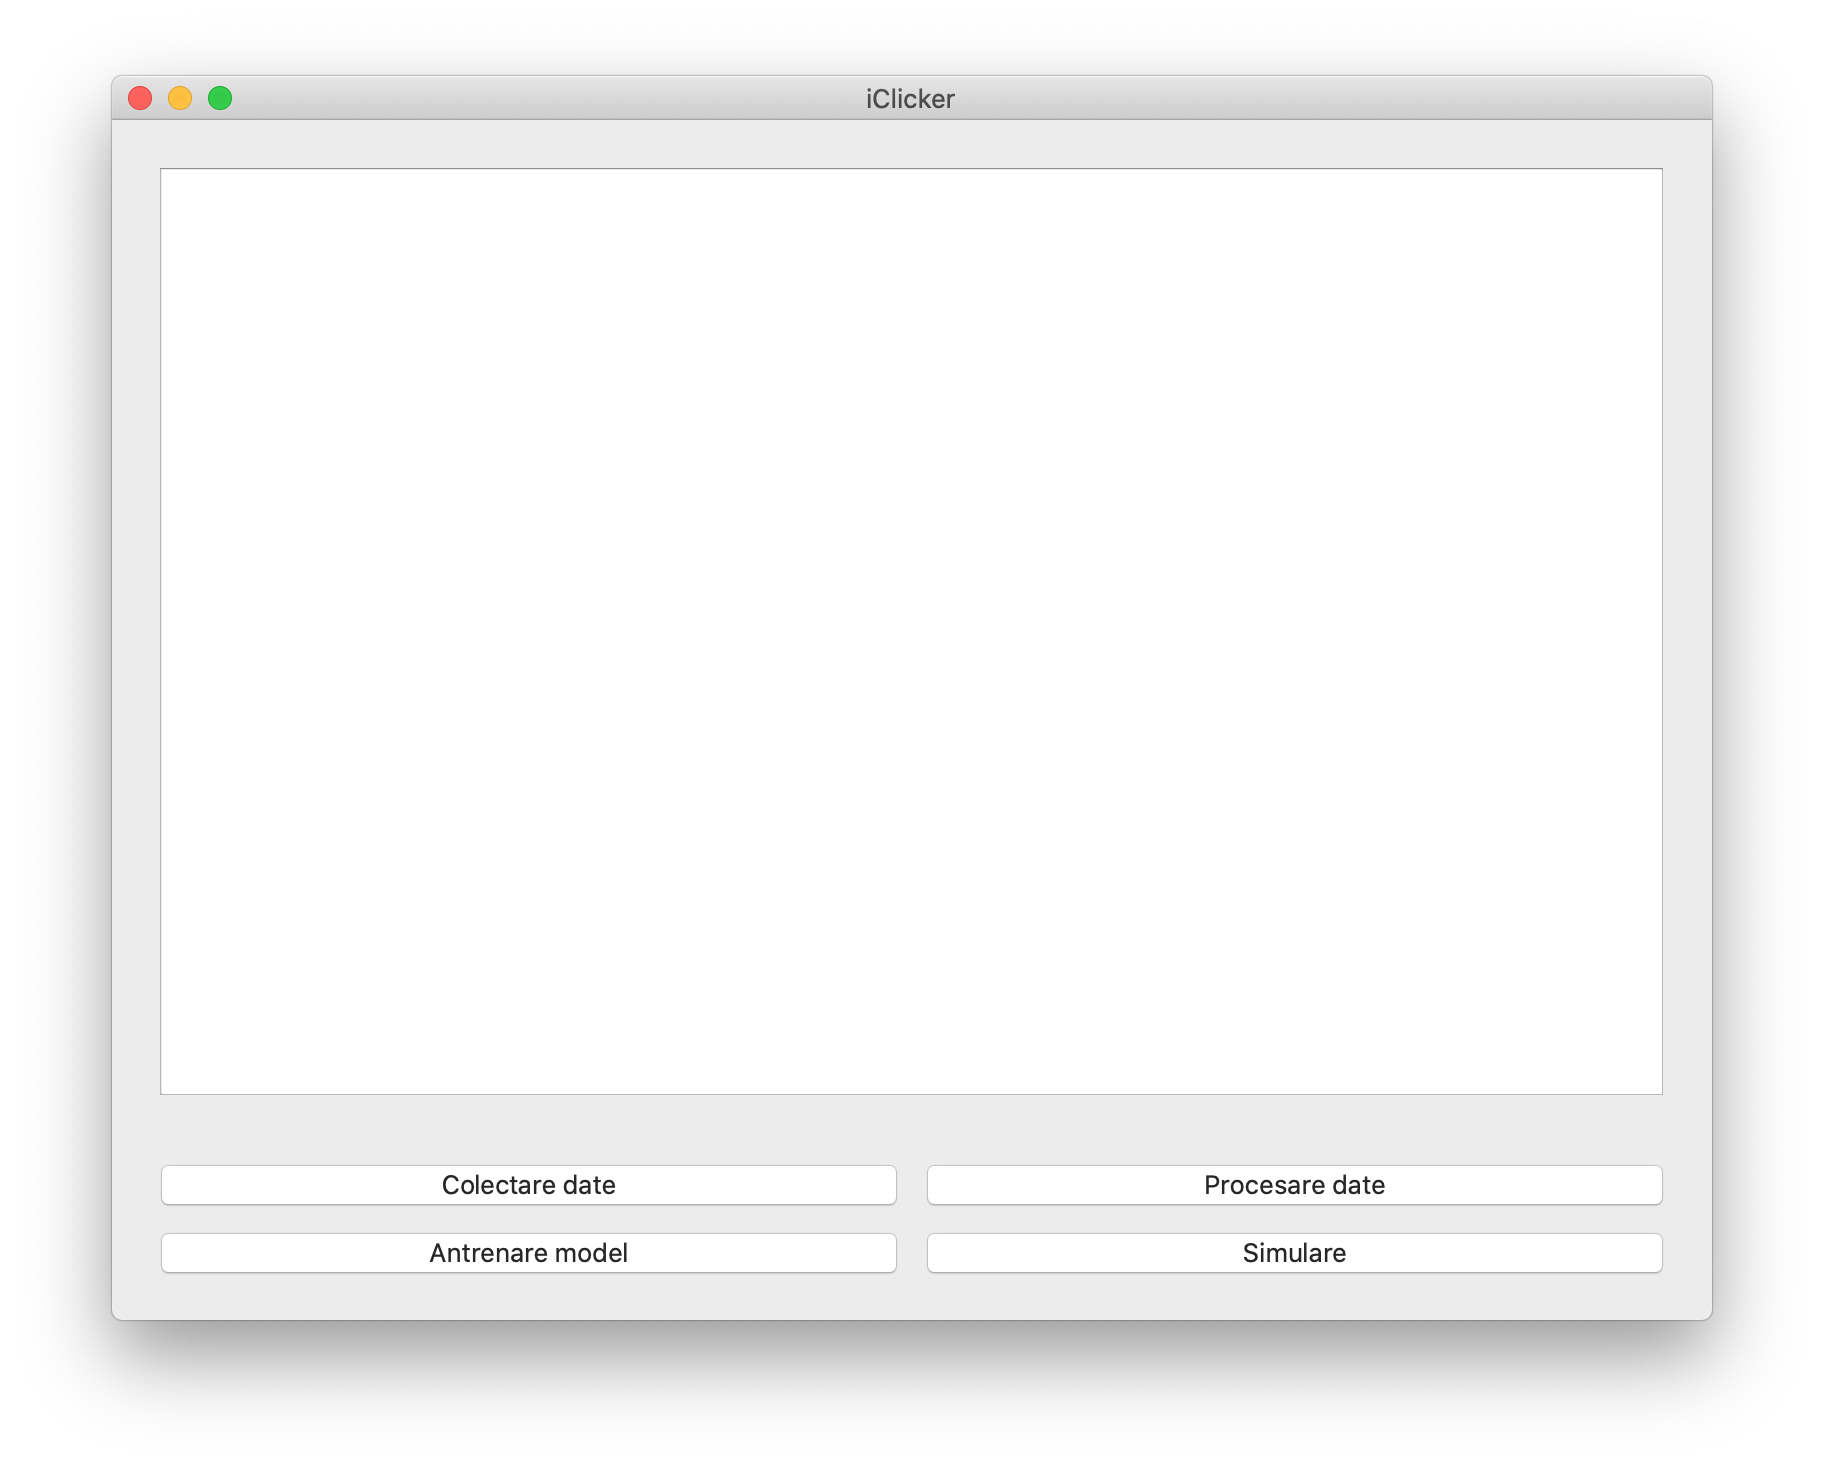
\includegraphics[width=\textwidth]{iClicker.png}
    \caption{Fereastra principală a aplicației}
\end{figure}

Pentru a realiza funcția de colectare a datelor, utilizatorul trebuie să apese pe butonul denumit sugestiv ``Colectare date''.
Există două moduri în care poate fi realizată această funcție: modul activ și modul pasiv.

Modul activ presupune ca utilizatorul să urmărească cursorul mouse-ului pe ecran în timp ce acesta se mișcă pe un traseu fix, prin mișcări glisante, de la stânga la dreapta, apoi de la dreapta la stânga, astfel încât să acopere toată suprafața ecranului.
De fiecare dată când cursorul își schimbă poziția, aplicația salvează o imagine preluată de la webcam împreună cu poziția cursorului în acel moment.
Pentru a evita obosirea ochilor și a asigura o colectare de date consistentă, utilizatorul poate lua o pauză (întreruperea mișcării cursorului) prin apăsarea tastei \emph{SPACEBAR}.
De asemenea, viteza cu care se mișcă cursorul poate fi schimbată prin apăsarea tastelor \emph{SĂGEATĂ SUS} și \emph{SĂGEATĂ JOS}.

Metoda pasivă este menită să nu deranjeze rutina utilizatorului, astfel încât de fiecare dată când utilizatorul apasă pe butonul stâng al mouse-ului, aplicația salvează, în același mod ca mai sus, o imagine capturată prin intermediul webcam-ului și poziția cursorului pe ecran.
Este important de menționat că de multe ori nu ne uităm acolo unde apăsăm cu mouse-ul, așa că, deși este o metodă gândită să ruleze pe fundal, este bine ca utilizatorul să țină cont de prezența acesteia și să realizeze apăsări de buton acolo unde se uită, pentru a construi \emph{date consistente}.

Partea de procesare de date și de antrenare a modelelor se folosesc în același mod, prin apăsarea butoanelor denumite sugestiv.
Acestea vor informa utilizatorul despre progresul realizat prin intermediul ferestrei principale.

Toate aceste funcționalități rulează pe câte un \emph{fir de execuție} separat.
Dacă acest lucru nu s-ar petrece, atunci firul principal de execuție (care se ocupă și de afișarea componentelor grafice) ar fi ``blocat'' până la terminarea execuției acelor funcționalități și aplicația ar ``îngheța''.

Ultima componentă este și cea mai importantă, cea de simulare a funcționalităților mouse-ului.
Prin intermediul acesteia, aplicația începe să urmărească ochii utilizatorului și să-i analizeze gesturile faciale.
Utilizatorului i se va arăta pe ecran și o grilă (de dimensiune 3x3) pentru a vedea în timp real predicțiile rețelei convoluționale legate de zona ecranului pe care acesta o privește.

Pentru a construi aplicația m-am ghidat după modelul de proiectare \emph{MVC} (\emph{Model–View–Controller}).
Fiecare componentă care poate fi folosită de utilizator are o interfață grafică atașată (\emph{View}) ce poate cere aplicației (prin intermediul unui \emph{Controller}) să realizeze anumite proceduri.
Partea de \emph{Model} al acestui tipar de dezvoltare constă în structurarea datelor colectate neprelucrate și a celor rezultate din partea de procesare a datelor.

\begin{figure}[ht]
    \centering
    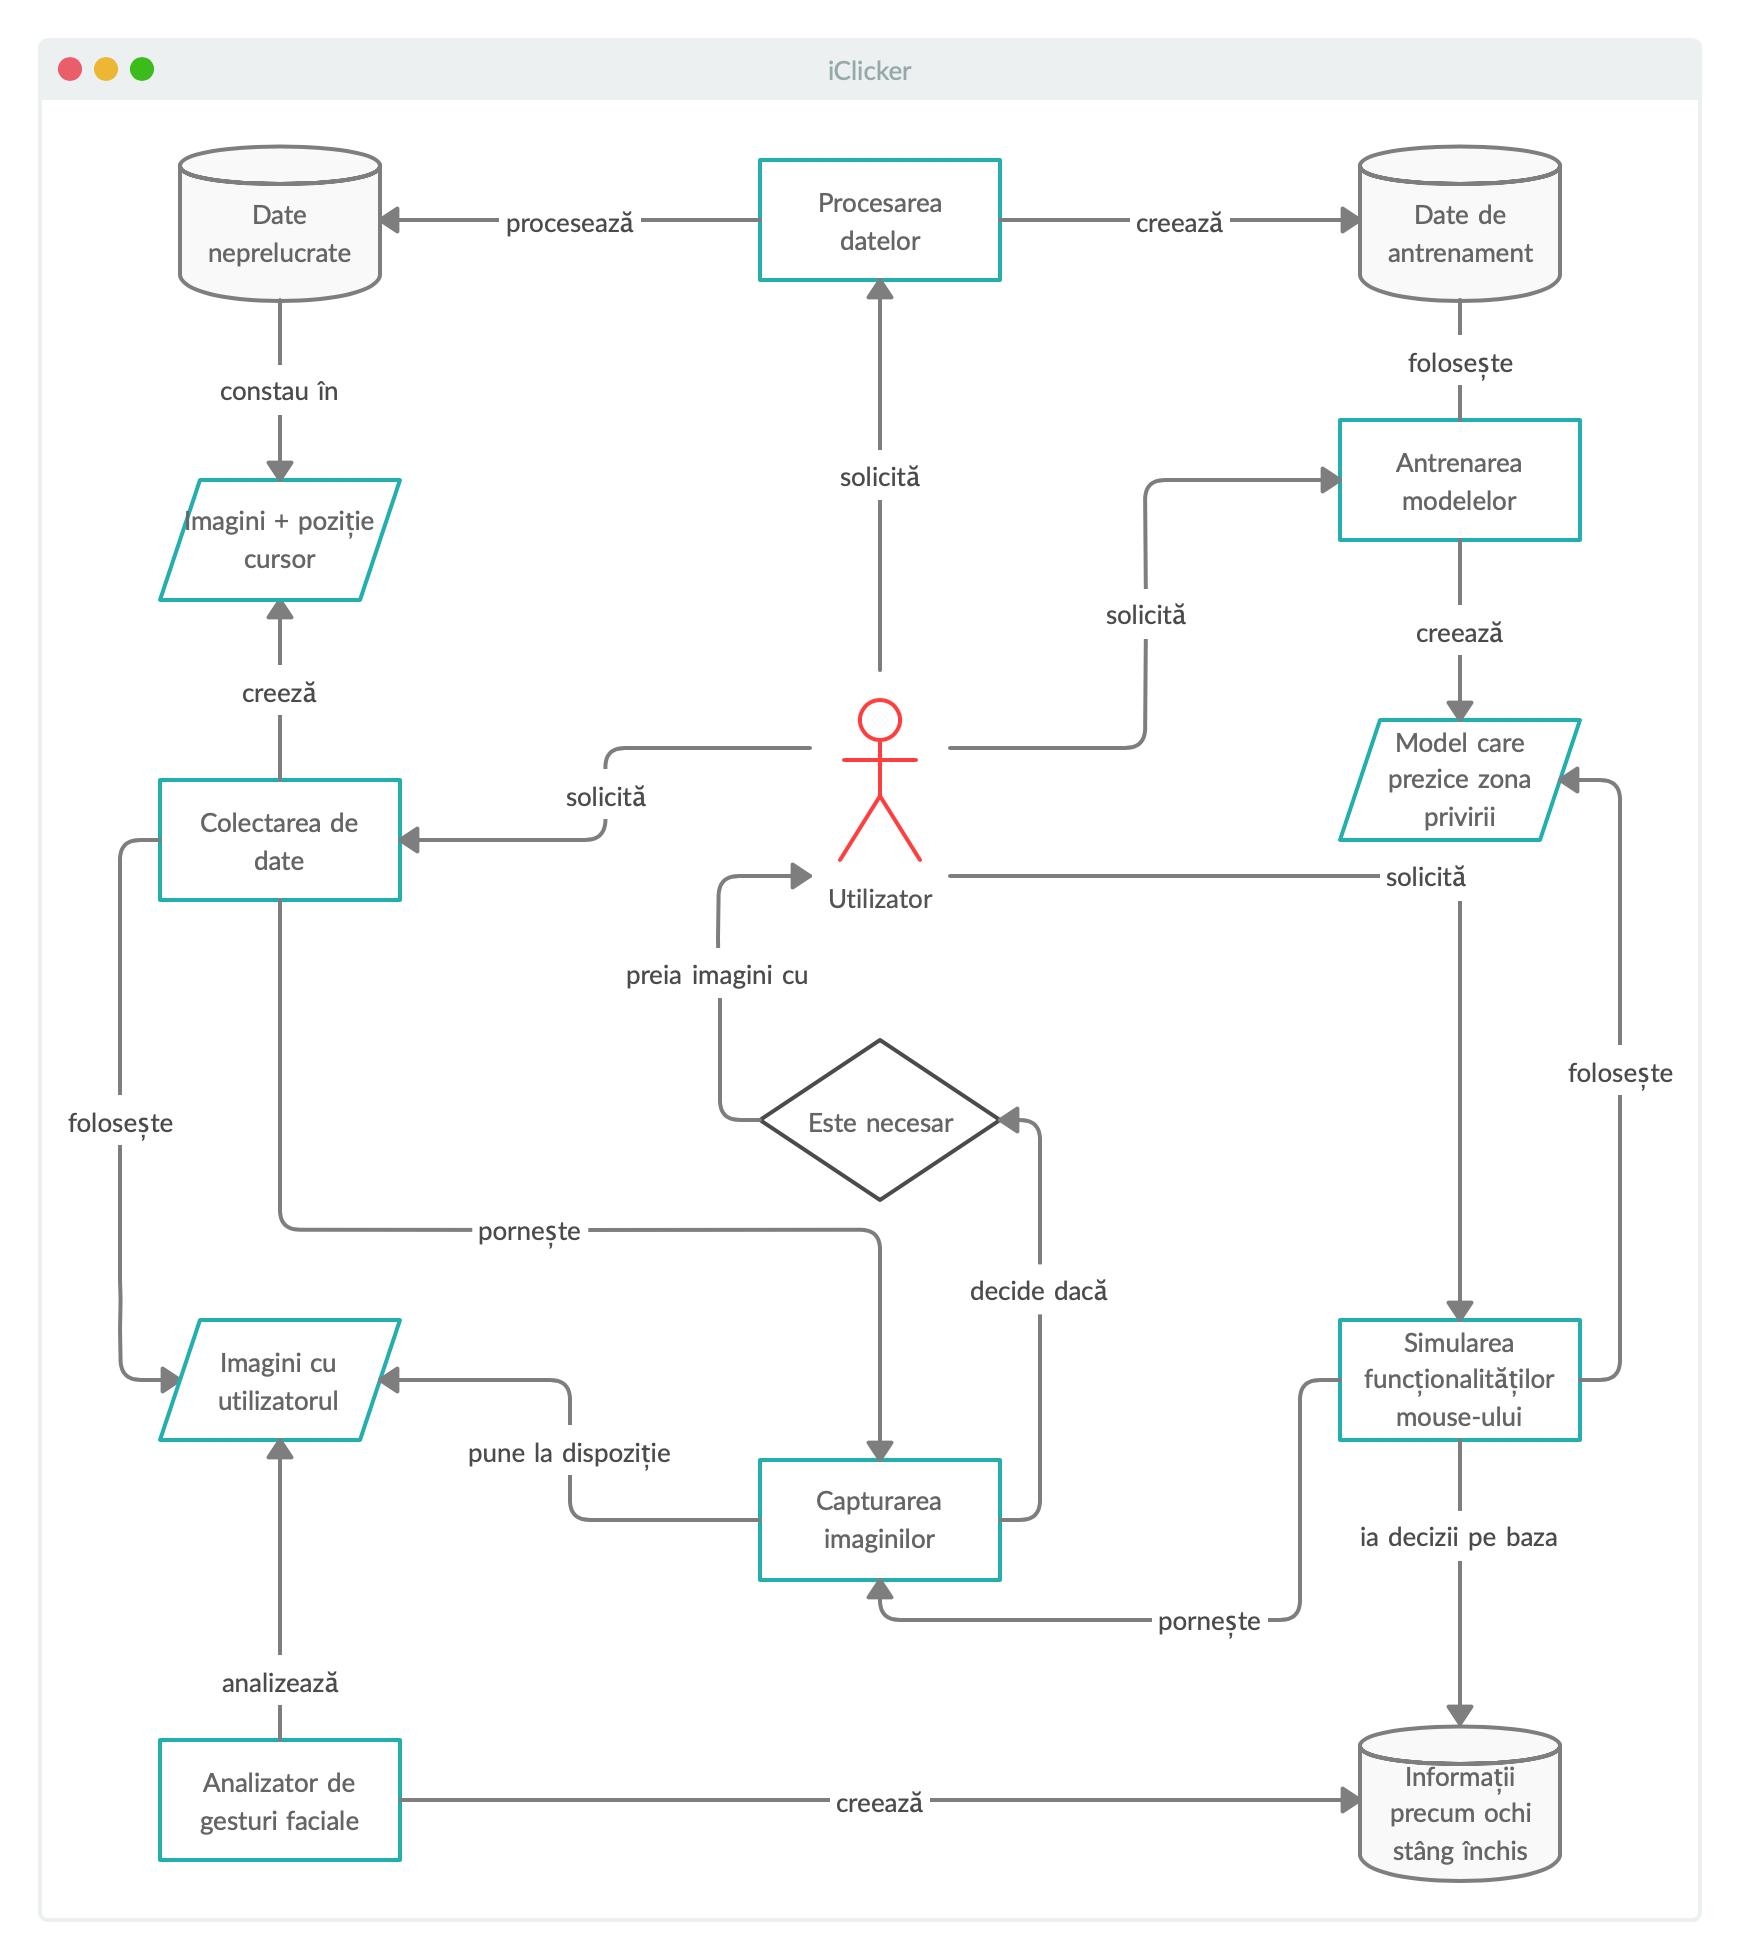
\includegraphics[width=\textwidth]{flowchart.png}
    \caption{Organigrama aplicației}
\end{figure}

    \chapter{Soluția propusă}
\label{chapter2}
\section{Informații preliminare}
\subsection{Informații tehnice}
Pentru dezvoltarea, structurarea și versionarea codului sursă al lucrării, am folosit platforma gratuită Github\footnote{\url{https://github.com}}.
\emph{Repository-ul} proiectului poate fi accesat la această adresă: \url{https://github.com/sergiuiacob1/iClicker/}.

Rezultatele prezentate aici au fost bazate pe imagini capturate prin intermediul unei camere webcam capabile de o rezoluție maximă HD (1280x720 pixeli).
Experimentele realizate au fost făcute în general în medii bine luminate, întrucât o dată cu scăderea intensității luminii suferă și utilitatea aplicației prezentate aici din cauza calității webcam-ului.

\subsection{Python \& Conda}
Unul dintre cele mai populare limbaje de programare când vine vorba de învățare profundă este Python\footnote{\url{https://www.python.org}}.
Astfel, am ales să dezvolt aplicația folosind acest limbaj, deoarece suportul din partea comunității este unul foarte bun și resursele găsite online pentru a rezolva probleme comune sunt vaste.
De asemenea, este un limbaj potrivit pentru teste, experimente și pentru o prototipizare rapidă a anumitor funcționalități, iar pe parcursul dezvoltării am făcut numeroase astfel de teste.

Am facut uz de asemenea de tehnologia Conda\footnote{\url{https://docs.conda.io/en/latest/}} care ajută în gestionarea mediilor de dezvoltare.
Cu ajutorul acestora am putut crea un mediu de dezvoltare separat, care se poate instala cu ușurință pe orice calculator fără a crea conflicte cu alte pachete deja existente pe mașina unui utilizator.
Această combinație a ajutat la îndeplinirea necesității aplicației de a rula pe mai multe sisteme de operare, întrucât Python deja satisface această nevoie.
Versiunile folosite au fost \lstinline{Python 3.7} și Conda \lstinline{4.8.0}.

\subsection{OpenCV}
Una dintre bibliotecile Python care au adus funcționalități cruciale acestui proiect este OpenCV\footnote{\url{https://pypi.org/project/opencv-python/}}.
Aceasta conține diferite funcționalități legate de Viziunea Computerizată, precum captura de imagini prin intermediul webcam-ului.
Am folosit-o de asemenea pentru a realiza redimensionări de imagini, pentru a le converti în gri sau în imagini alb-negru prin aplicarea unui \emph{binary threshold}.
Versiunea folosită a fost \lstinline{4.1.2}.

\subsection{PyQt5}
Aplicația dezvoltată are și o interfață grafică ce a fost implementată folosind biblioteca PyQt5\footnote{\url{https://pypi.org/project/PyQt5/}}.
Unul dintre avantajele acestei biblioteci este acela că oferă un nivel înalt de abstractizare și componentele (butoanele, ferestrele etc.) grafice au un aspect diferit în funcție de sistemul de operare pe care rulează aplicația, fără a fi nevoie ca acest lucru să fie implementat de dezvoltator.
Versiunea folosită a fost \lstinline{5.14}.

\subsection{Keras \& PyTorch}
Keras\footnote{\url{https://keras.io}} și PyTorch\footnote{\url{https://pytorch.org}} au fost folosite pentru a facilita antrenarea rețelelor neuronale (de tip \emph{MLP} sau \emph{CNN}).
Acestea au mărit cu mult realizarea arhitecturilor pentru învățarea automată, Keras având un nivel de abstractizare decât PyTorch.
Am folosit cele două tehnologii pentru a căpăta experiență în utilizarea amândurora, întrucât nu există o ``cea mai bună unealtă'', ci mai degrabă contextul nevoii dictează uneltele, tehnologiile ce ar trebui folosite.
Versiunile folosite au fost Keras \lstinline{2.2.4} și PyTorch \lstinline{1.4}.

\subsection{dlib}
Cea mai importantă bibliotecă de care am făcut uz în această lucrare este dlib\footnote{\url{https://pypi.org/project/dlib/}}.
Cu ajutorul acesteia, am putut realiza identificarea reperelor faciale într-o imagine care conținea fața unei persoane.
Reperele respective sunt furnizate de către sub forma unei liste de coordonate $(x, y)$ corespunzătoare pixelilor acelor caracteristici faciale.
Mai departe, pe baza acestora, am putut decupa fie fața, fie ochii persoanei în imagini mai mici pe care le-am folosit mai apoi ca date de antrenament.
Versiunea folosită a fost \lstinline{19.19.0}.

\section{Limite și constrângeri}
Aplicația are niște limite și lucrează de asemenea cu niște presupuneri, precum faptul că utilizatorul folosește un singur monitor și un singur webcam.
De asemenea, imaginile folosite sunt cu mine însumi, deci trebuie luat în vedere acest lucru pentru orice rezultat prezentat.

Aplicația este menită să se poată ``mula'' pe fizionomia utilizatorului, însă este posibil să aibă performanțe mai slabe pentru persoanele care poartă ochelari, spre exemplu.
Motivul pentru care se întâmplă acest lucru este acela că aplicația lucrează cu ochii utilizatorului, iar dacă lumina se reflectă în lentilele ochelarilor, ochii ar putea fi indistinctibili.
Ca o ultimă mențiune, aplicația se concentrează majoritar pe poziția pupilelor relativ la ochi (glob ocular + anexe ale globului ocular), deci se va considera că poziția capului nu va suferi schimbări majore între datele de antrenament și datele de test.

\section{Structura aplicației}
Aplicația are 4 mari componente, corespunzătoare pașilor luați în rezolvarea unei probleme de învățarea automată: colectarea de date, procesarea acestora, antrenarea unui model care realizează urmărirea ochilor și simularea funcționalităților mouse-ului.
Utilizatorul poate interacționa cu aceste componente prin intermediul interfaței grafice realizată în PyQt5.
Fereastra principală a aplicației are și o parte în care vor fi afișate informații utile.

Pentru a construi aplicația m-am ghidat după modelul de proiectare \emph{MVP} (\emph{Model–View–Presenter}).
Fiecare componentă care poate fi folosită de utilizator are o interfață grafică atașată (\emph{View}) ce poate cere aplicației (prin intermediul unui \emph{Presenter}) să realizeze anumite proceduri.
Partea de \emph{Model} al acestui șablon de dezvoltare constă în datele colectate neprelucrate și a celor rezultate din partea de procesare a datelor, precum și în modelele antrenate folosind aceste date.

\begin{figure}[ht]
    \centering
    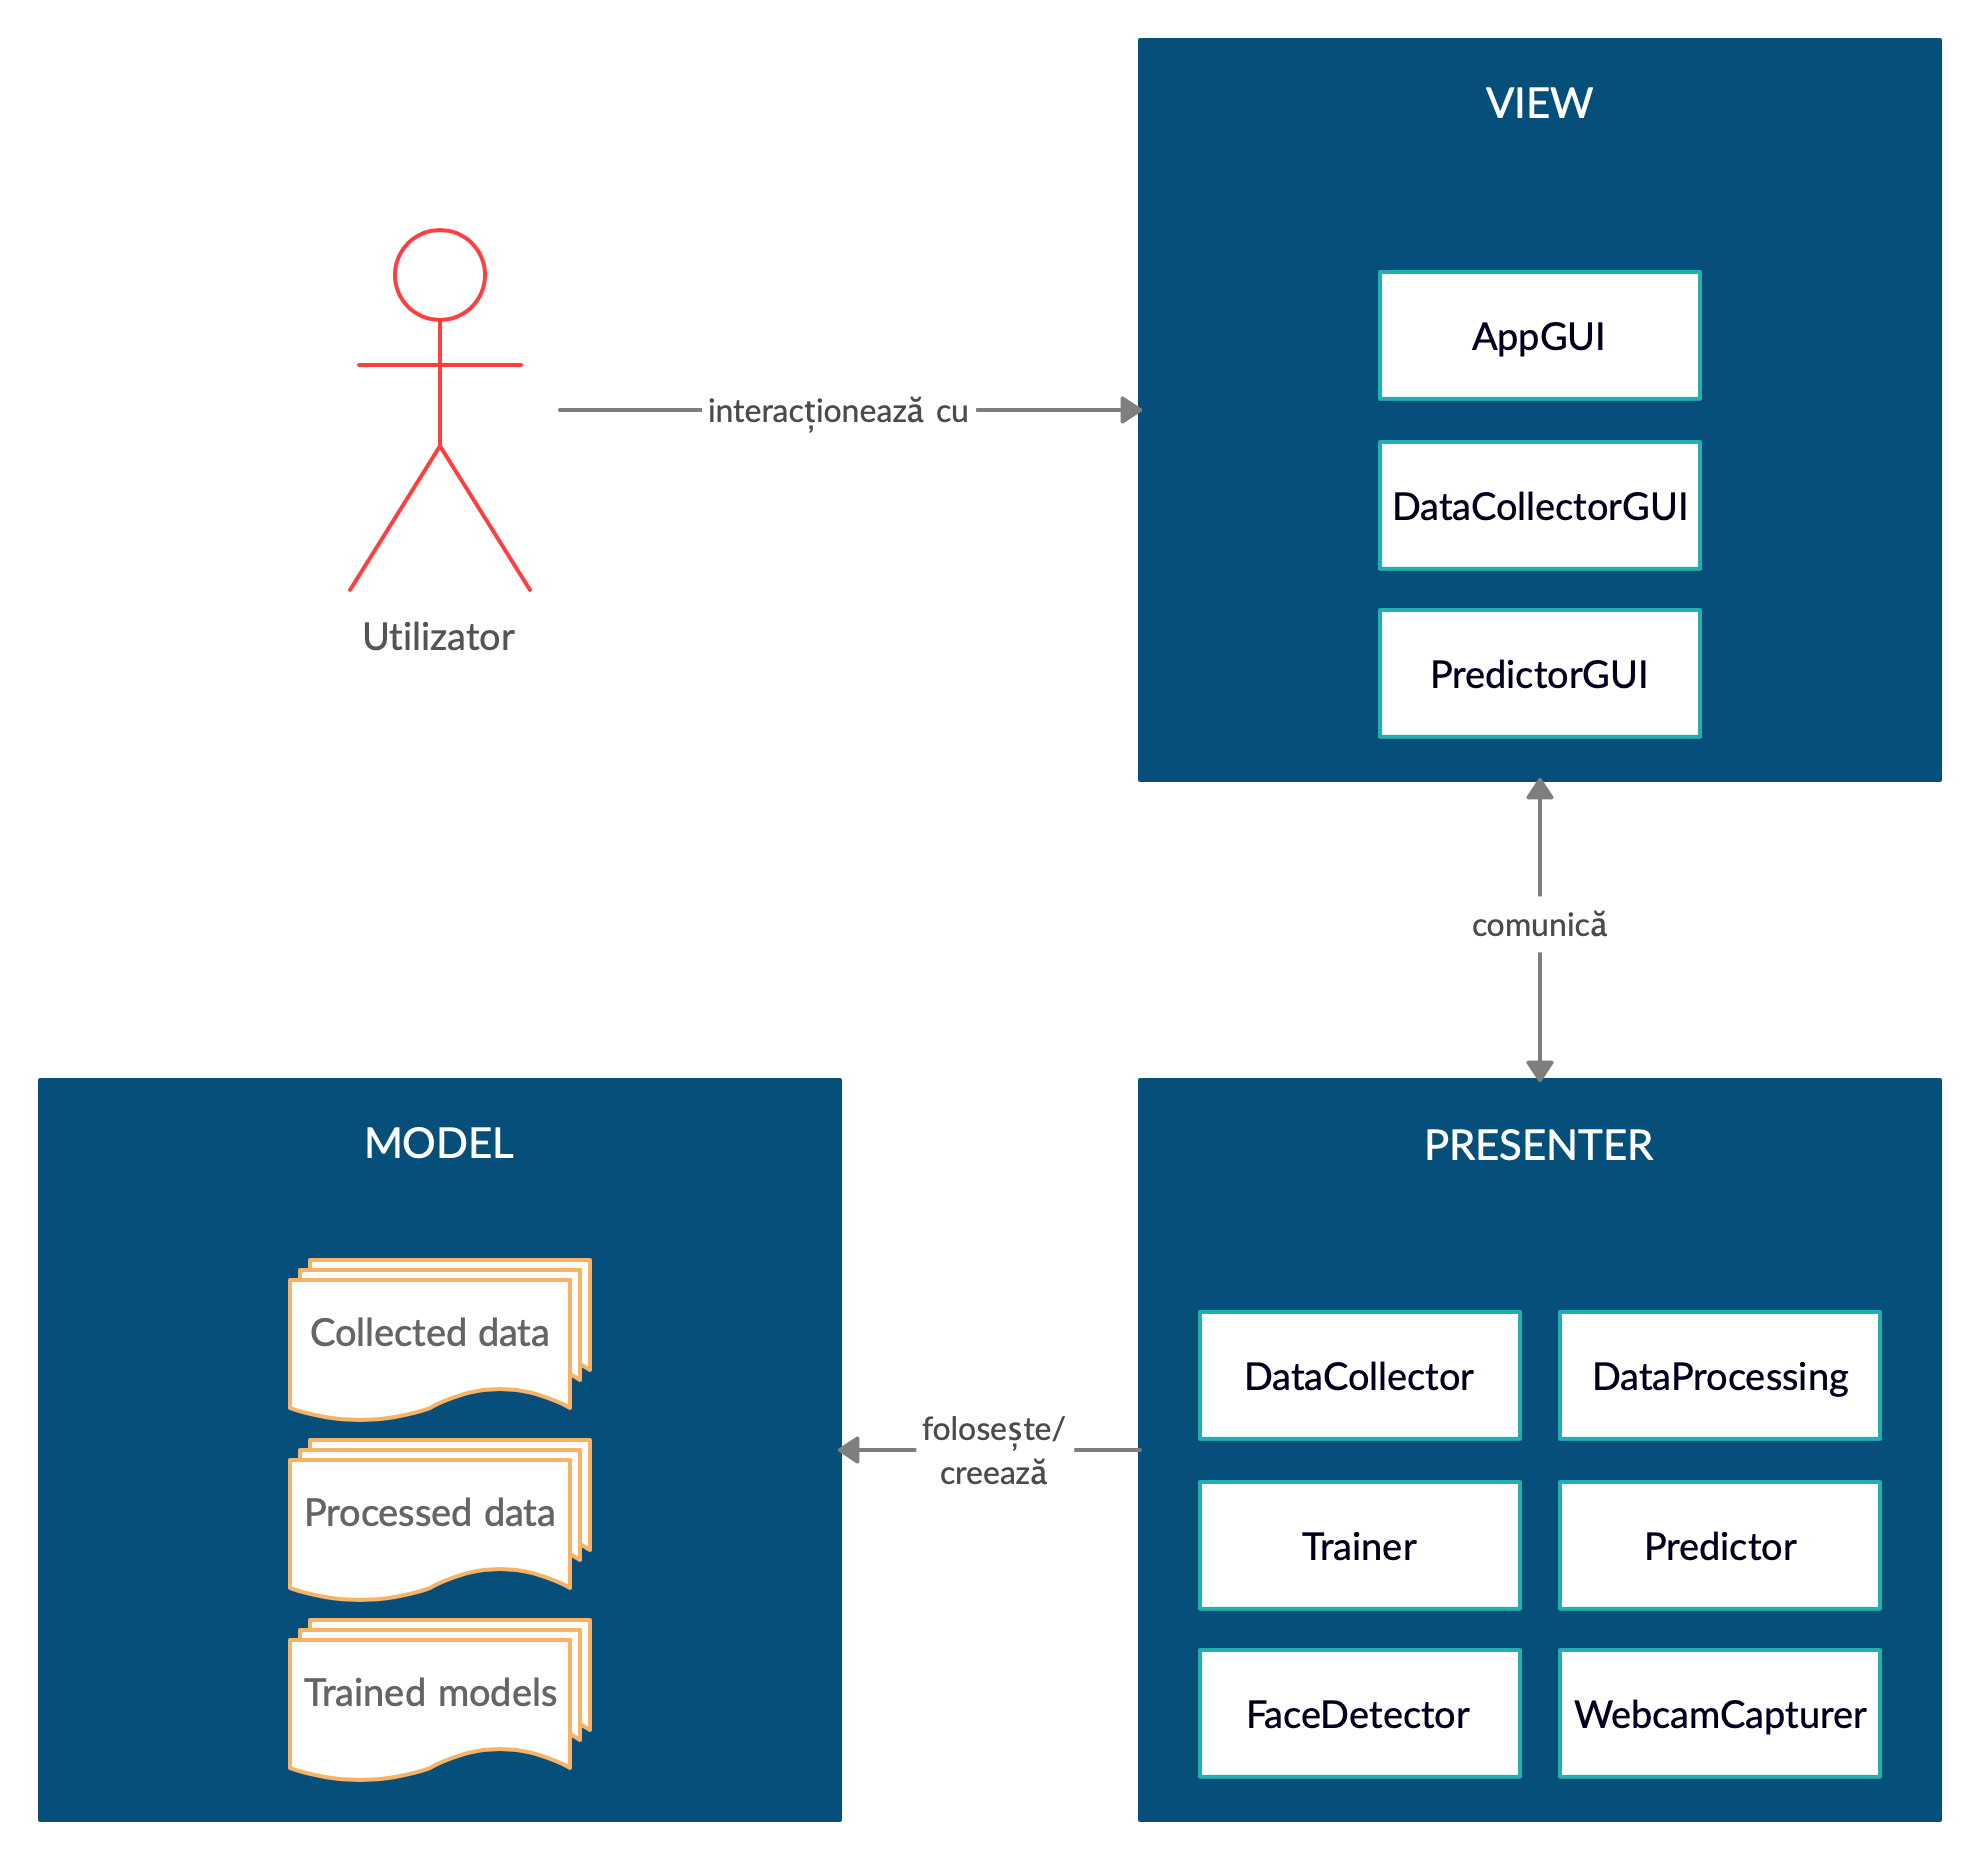
\includegraphics[width=\textwidth]{mvp.png}
    \caption{Arhitectura MVP a aplicației}
\end{figure}

\begin{figure}[ht]
    \centering
    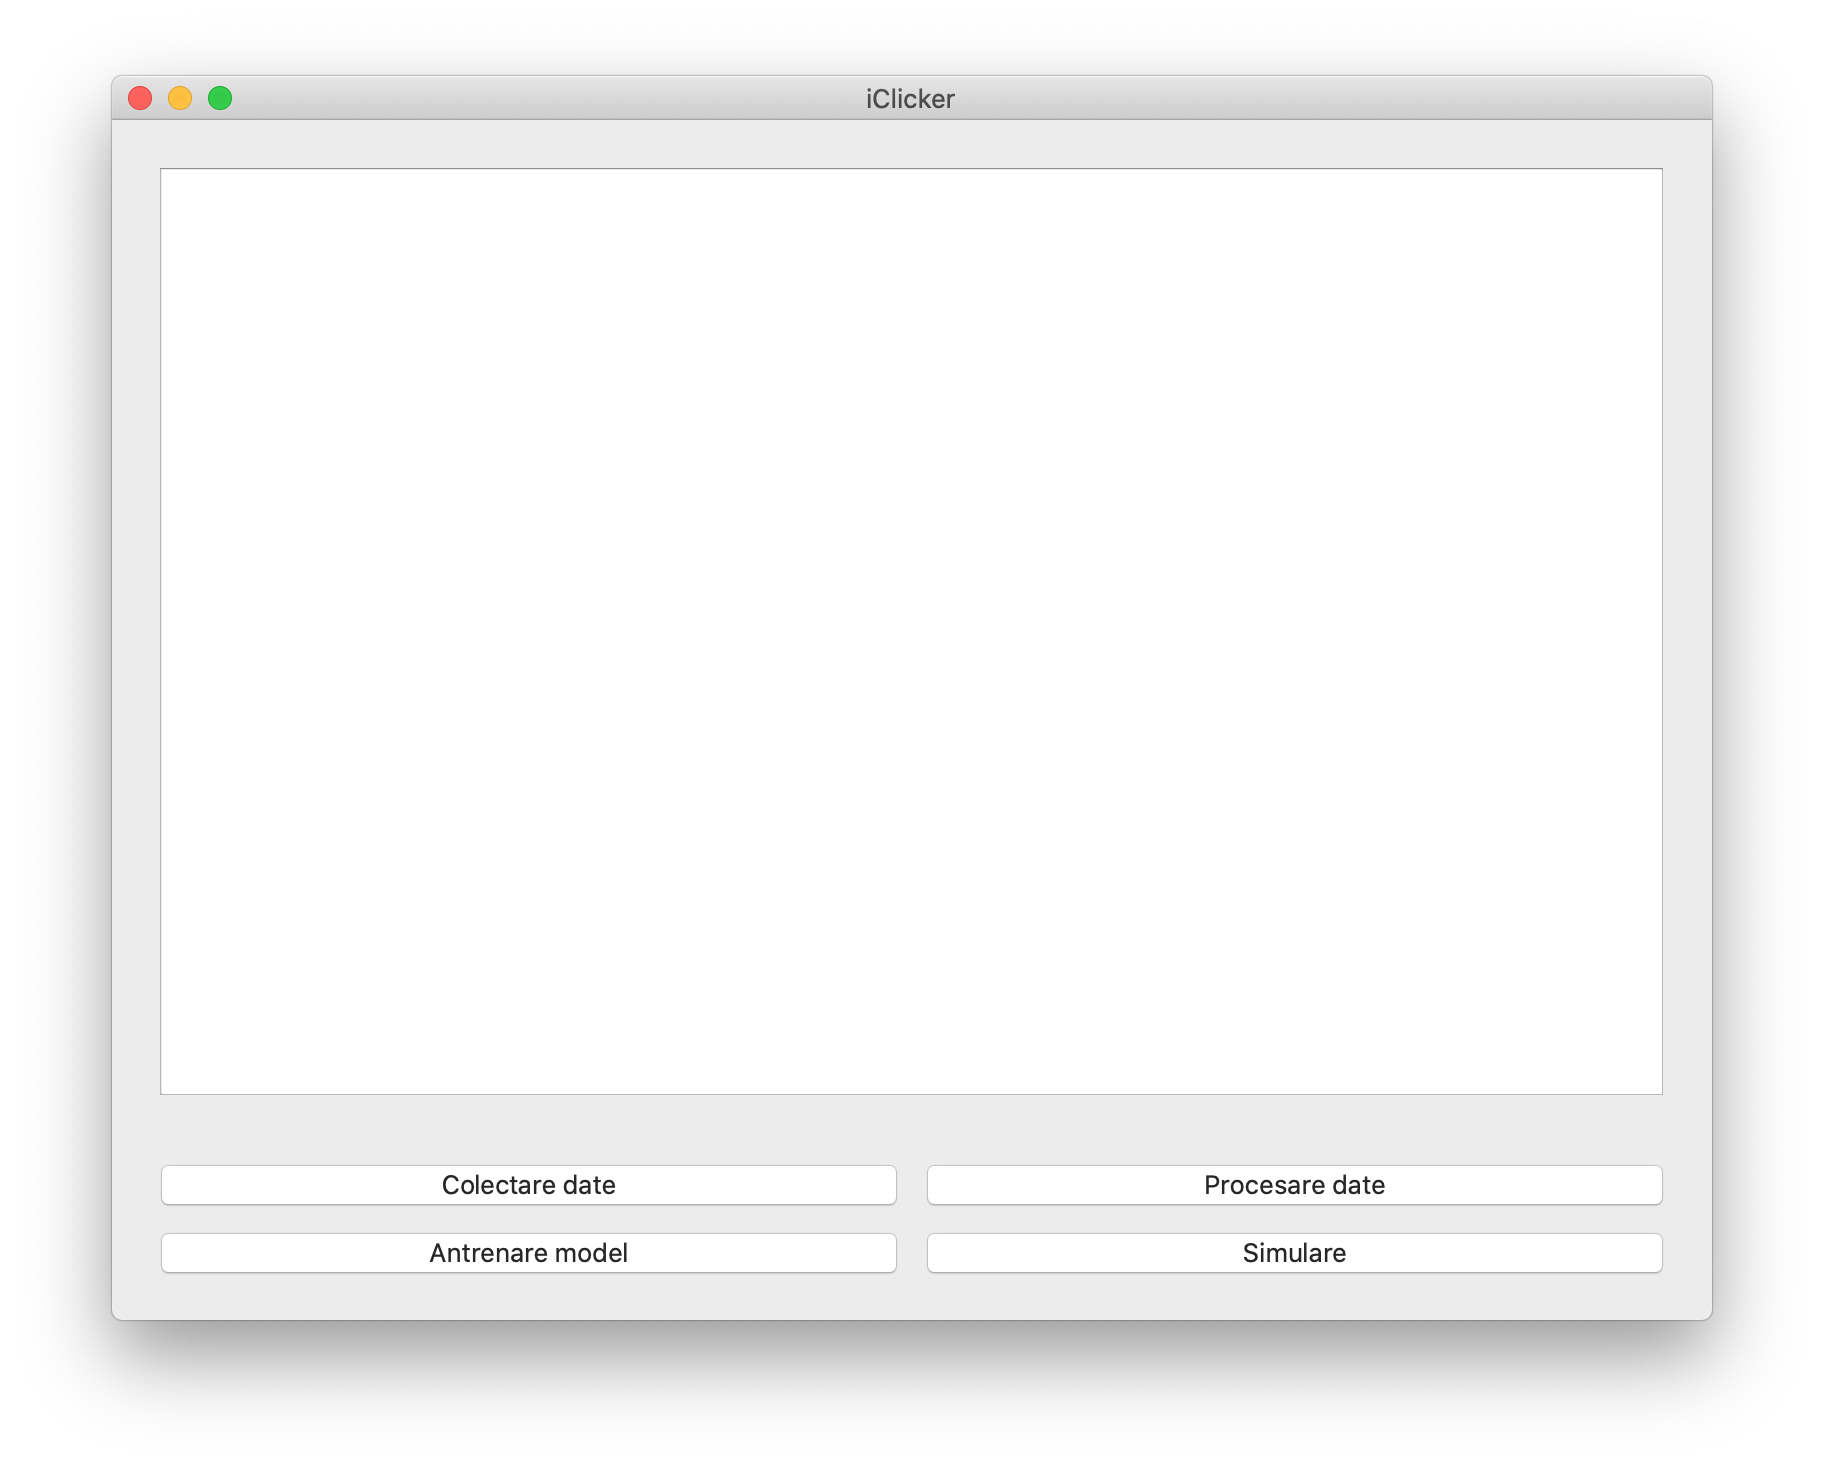
\includegraphics[width=\textwidth]{iClicker.png}
    \caption{Fereastra principală a aplicației}
\end{figure}

\begin{figure}[ht]
    \centering
    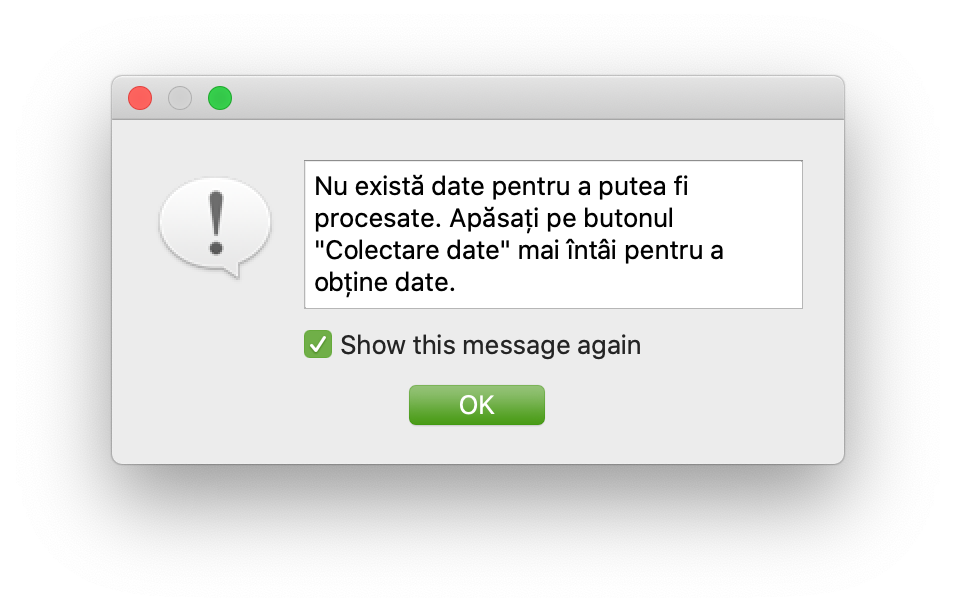
\includegraphics[width=0.32\textwidth]{err1.png}
    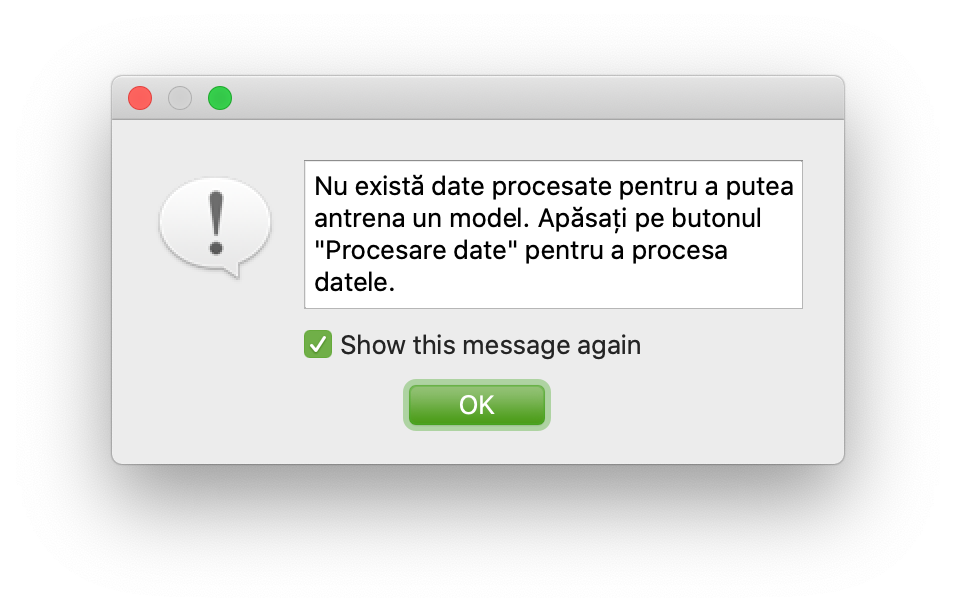
\includegraphics[width=0.32\textwidth]{err2.png}
    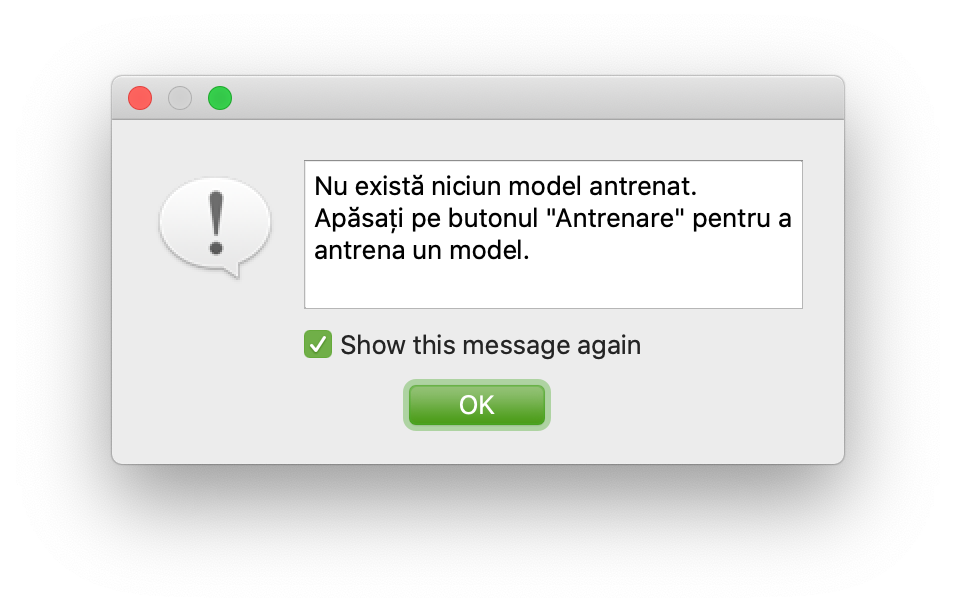
\includegraphics[width=0.32\textwidth]{err3.png}
    \caption{Mesaje de eroare}
\end{figure}

Pentru a realiza funcția de colectare a datelor, utilizatorul trebuie să apese pe butonul denumit sugestiv ``Colectare date''.
Există două moduri în care poate fi realizată această funcție: modul activ și modul pasiv.

Modul activ presupune ca utilizatorul să urmărească cursorul mouse-ului pe ecran în timp ce acesta se mișcă pe un traseu fix, prin mișcări glisante, de la stânga la dreapta, apoi de la dreapta la stânga, astfel încât să acopere toată suprafața ecranului.
De fiecare dată când cursorul își schimbă poziția, aplicația salvează o imagine preluată de la webcam împreună cu poziția cursorului în acel moment.
Pentru a evita obosirea ochilor și a asigura o colectare de date consistentă, utilizatorul poate lua o pauză (întreruperea mișcării cursorului și a colectării datelor) prin apăsarea tastei \emph{SPACEBAR}.
De asemenea, viteza cu care glisează cursorul poate fi schimbată prin apăsarea tastelor \emph{SĂGEATĂ SUS} și \emph{SĂGEATĂ JOS}.

Metoda pasivă este menită să nu deranjeze rutina utilizatorului, astfel încât de fiecare dată când utilizatorul apasă pe butonul stâng al mouse-ului, aplicația salvează, în același mod ca mai sus, o imagine capturată prin intermediul webcam-ului și poziția cursorului pe ecran.
Această variantă poate fi contraintuitivă, având în vedere că aplicația ar trebui folosită fără ajutorul mâinilor, dar m-a ajutat pe mine în obținerea datelor în timp ce realizam alte sarcini.
Este important de menționat că de multe ori nu ne uităm acolo unde apăsăm cu mouse-ul, așa că, deși este o metodă gândită să ruleze pe fundal, este bine ca utilizatorul să țină cont de prezența acesteia și să realizeze apăsări de buton acolo unde se uită, pentru a construi \emph{date consistente}.

Partea de procesare de date și de antrenare a modelelor se folosesc în același mod, prin apăsarea butoanelor denumite sugestiv.
Acestea vor informa utilizatorul despre progresul realizat prin intermediul ferestrei principale.

Toate aceste funcționalități rulează pe câte un \emph{fir de execuție} separat.
Dacă acest lucru nu s-ar petrece, atunci firul principal de execuție (care se ocupă și de afișarea componentelor grafice) ar fi ``blocat'' până la terminarea execuției acelor funcționalități și aplicația ar ``îngheța''.

Ultima componentă este și cea mai importantă, cea de simulare a funcționalităților mouse-ului.
Prin intermediul acesteia, aplicația începe să urmărească ochii utilizatorului și să-i analizeze gesturile faciale.
Utilizatorului i se va arăta pe ecran și o grilă (de dimensiune 3x3) pentru a vedea în timp real predicțiile rețelei convoluționale legate de zona ecranului pe care acesta o privește.

\begin{figure}[H]
    \centering
    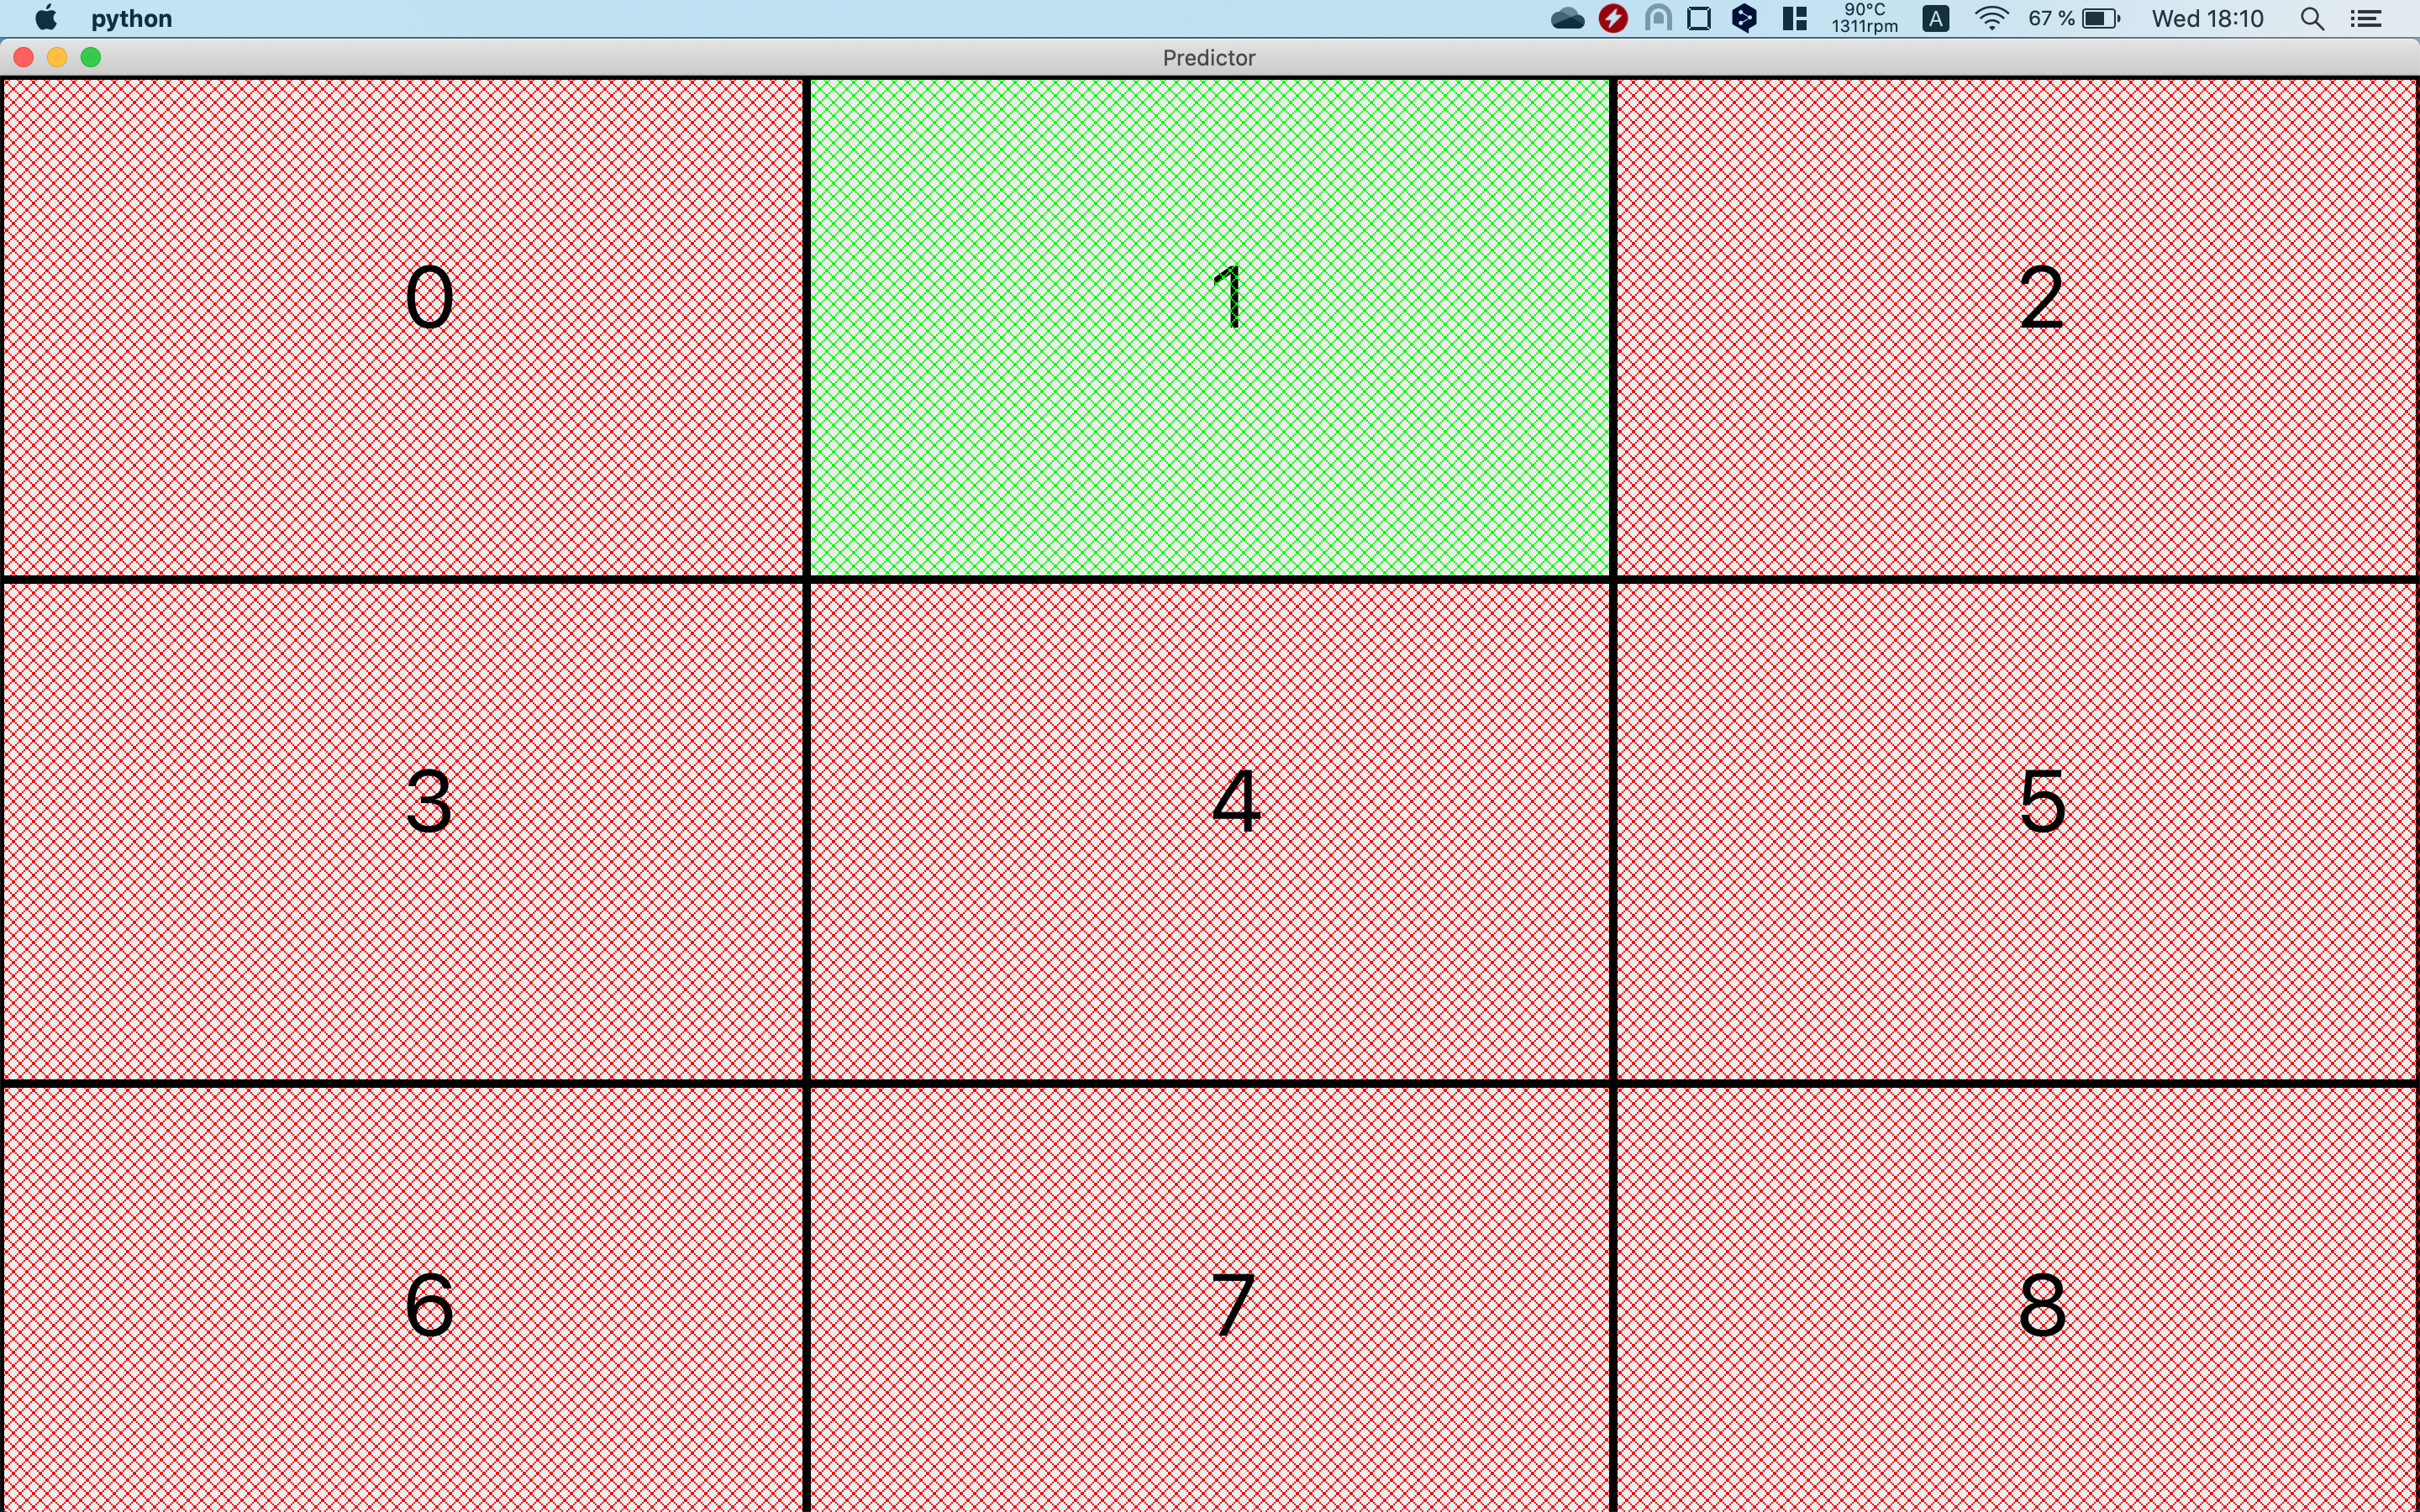
\includegraphics[width=0.49\textwidth]{pred1.png}
    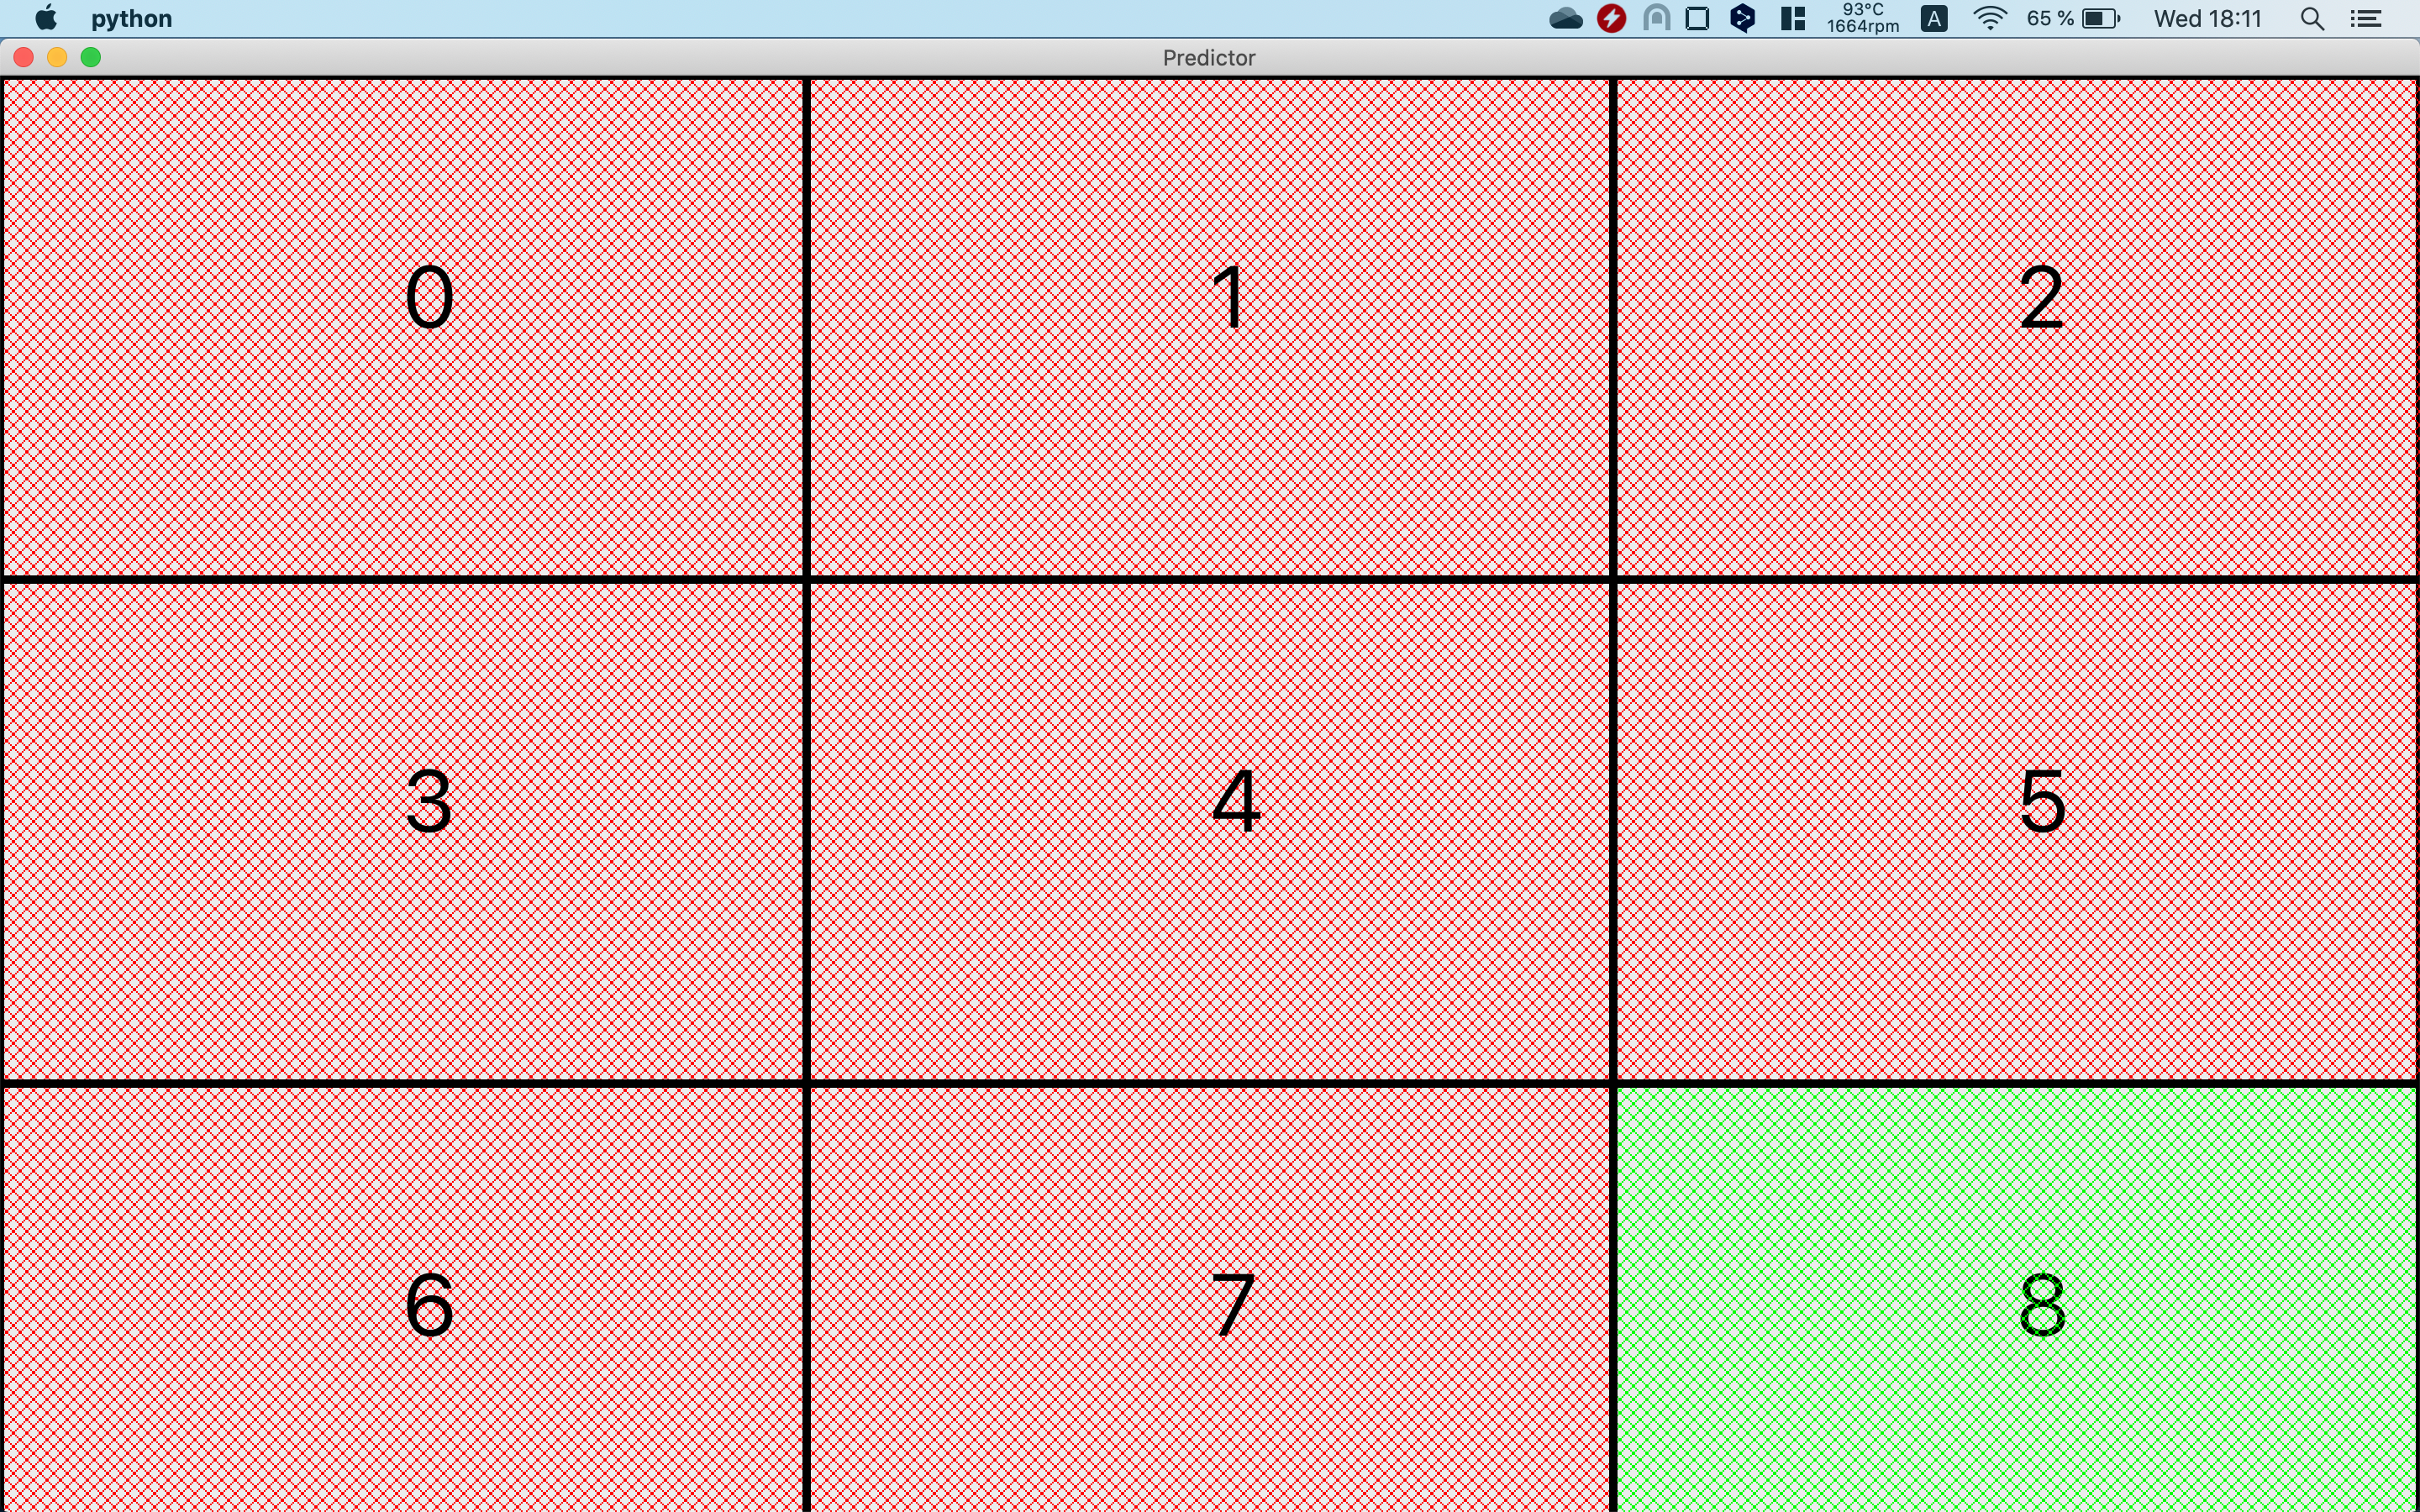
\includegraphics[width=0.49\textwidth]{pred2.png}
    \caption{Testarea predicțiilor ale zonei de privire ale utilizatorului}
\end{figure}

\begin{figure}[ht]
    \centering
    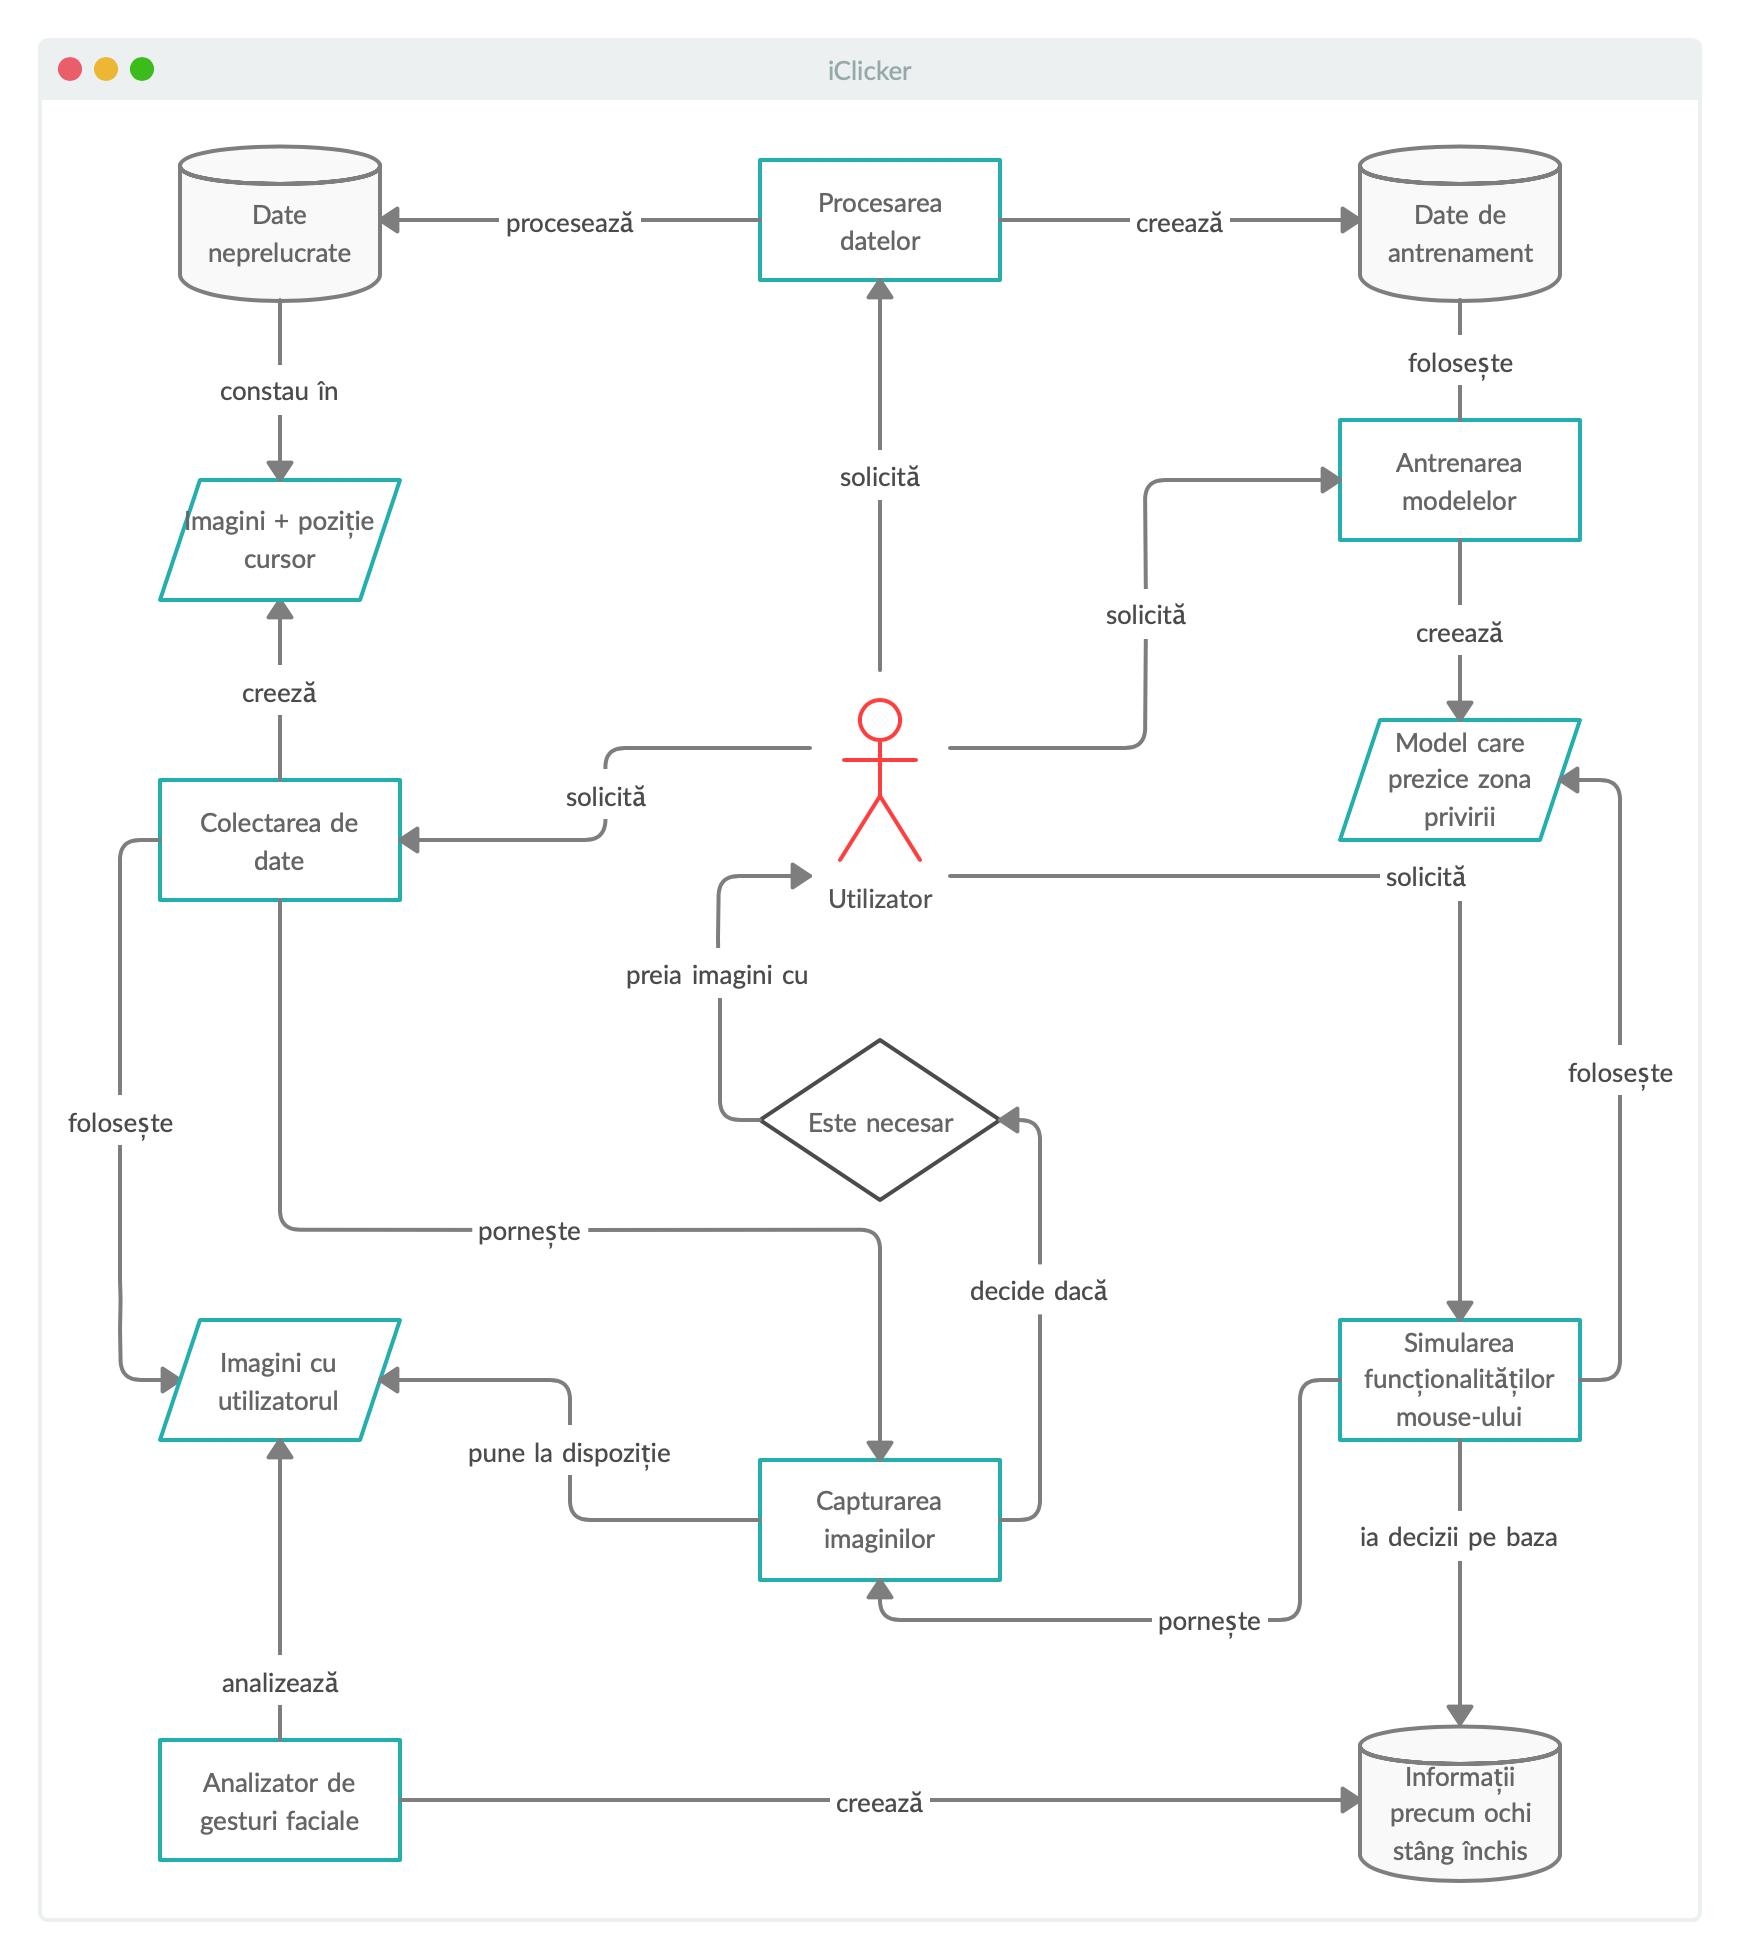
\includegraphics[width=\textwidth]{flowchart.png}
    \caption{Organigrama aplicației}
\end{figure}

    \chapter{Antrenament}
\section{Rețele MLP}

Primele experimente pe care le-am efectuat au fost efectuate folosind imaginile din care am extras ochii, pe care i-am convertit în imagini alb-negru (binary threshold), așa cum a fost menționat în prima parte a secțiunii de procesare de date\ref{data-processing:eyes}.
Fiecare ochi a fost redimensionat la 60x30 pixeli apoi au fost uniți orizontal, formând o imagine alb-negru de dimensiune 120x30 pixeli.
De asemenea, am etichetat fiecare imagine cu numărul celulei în care se uita utilizatorul, conform dimensiunii grilei folosite\ref{grid-example}.
Scopul a fost de a prezice, pentru imagini noi, numărul acelei celule.
Iată prima arhitectură pe care am încercat-o:

\begin{lstlisting}[language=Python, caption=Arhitectura MLP]
model = Sequential([
    Dense(100, input_shape=(n,), kernel_initializer='glorot_uniform'),
    Dropout(0.5),
    ReLU(),
    Dense(128, kernel_initializer='glorot_uniform'),
    Dropout(0.5),
    ReLU(),
    Dense(64, kernel_initializer='glorot_uniform'),
    # Dropout(0.5),
    ReLU(),
    Dense(Config.grid_size * Config.grid_size, activation='softmax')
])
\end{lstlisting}

\paragraph{Important}
Pentru primele experimente din această secțiune am folosit doar imaginile în care utilizatorul se uita în colțurile ecranului.
De exemplu, pentru o grilă de dimensiune 3x3, am ales doar imaginile în care eticheta corespunzătoare a imaginii este $0, 2, 6$ sau $8$.
Ultima mențiune este că datele de antrenament reprezintă $80\%$ din mulțimea totală de date, restul fiind date de testare.

\begin{center}
    \begin{tabular}{ c | c | c | c | c | c | c }
        \hline
        Experiment & Dim. grilă & Nr. imagini & Epoci & Optimizator & Rată învățare & Batch size \\ 
        \hline
        1 & 2x2 & 2184 & 300 & Adam & 0.001 & 32 \\
        \hline
        2 & 3x3 & 1247 & 300 & Adam & 0.001 & 32 \\
        \hline
        3 & 4x4 & 711 & 300 & Adam & 0.001 & 32 \\
        \hline
    \end{tabular}
\end{center}

Experimentele 2 și 3 au beneficiat de mai puține imagini de antrenament deoarece, dimensiunea grilei fiind mai mare, imaginile sunt mai dispersate și fiecare celulă are mai puține imagini corespunzătoare ei.
Evident, pentru o grilă 2x2, fiecare imagine se află intr-o celulă din colț (fiind doar 4), deci au fost folosite toate imaginile.

Primul rezultat pe care l-am constatat a fost că doar primul model putea prezice bine zona în care mă uitam.
Rețeaua MLP se descurca cu atât mai bine cu cât deschideam ochii mai mult, întrucât putea realiza mai bine conturul ochiului și să delimiteze pupila.

\begin{figure}[ht]
    \centering
    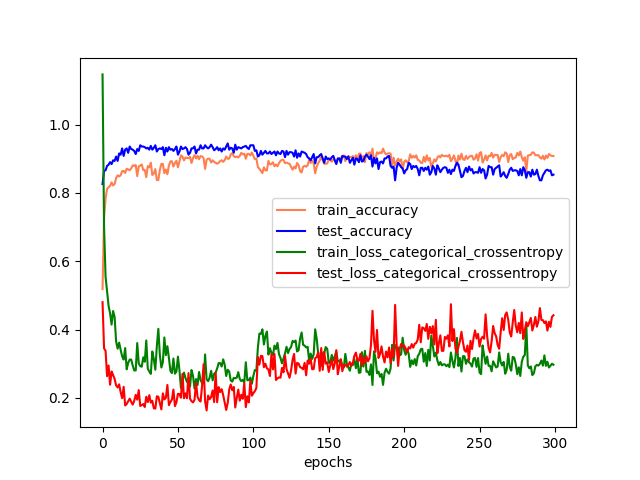
\includegraphics[width=0.49\textwidth]{graphs/model_1.png}
    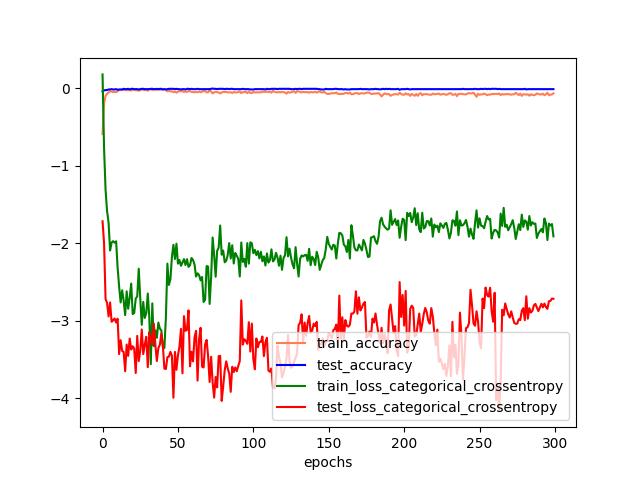
\includegraphics[width=0.49\textwidth]{graphs/model_2.png}
    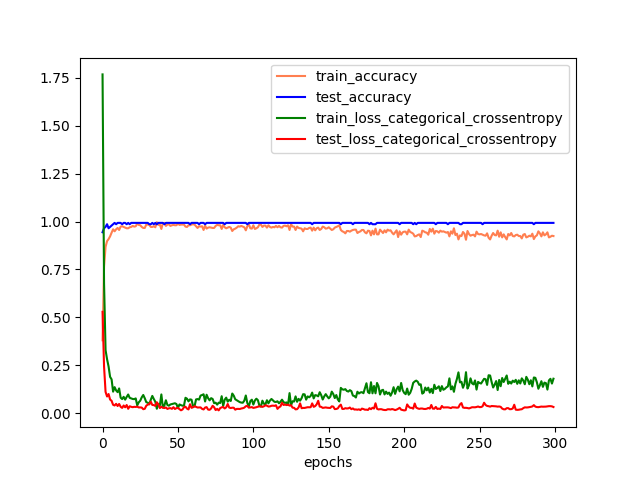
\includegraphics[width=\textwidth]{graphs/model_3.png}
    \caption{Modelele 1, 2 și 3}
\end{figure}

Acuratețea este foarte bună în cele 3 cazuri, însă nu se comportă atât de bine pe imagini noi, într-un mediu diferit.
De asemenea, am constatat ca luminozitatea și modul în care utilizatorul este plasat față de webcam sunt foarte importante și influențează performanța semnificativ.

Un lucru important de observat, care se va regăsi în majoritatea graficelor, sunt acele oscilații, alternanțe ale acurateței, care urcă și coboară.
Stratul \emph{Dropout} este cel care cauzează acest comportament, prin modul în care funcționează: ``by randomly dropping units during training to prevent their co-adaptation'', precum este menționat de \cite{dropout_algorithm}.
Acesta elimină neuroni ai unui strat, în mod aleatoriu, pentru a permite tuturor neuronilor să participe la învățare și să sporească performanța rețelei.
Astfel, atunci când sunt eliminați neuroni ``buni`'', adică aceia care conțin multă informație utilă pentru rezultatul final, performanța (acuratețea, eroarea) pot fi afectate negativ.
Pe de cealaltă parte, atunci când sunt eliminați neuroni care nu ajută foarte mult pentru predicție, performanța nu este afectata prea mult.

Am continuat prin a antrena aceeași rețea, pe o grilă de dimensiune 3x3, dar de data aceasta folosind toate imaginile disponibile.
Totuși, acest lucru nu a ajutat foarte mult și am observat și că după o anumită epocă, rețeaua nu se mai comporta bine pe datele de test și apărea fenomenul de \emph{overfit}.
Acest lucru se poate observa pe graficul modelului 4, unde acuratețea pentru datele de antrenament și cea pentru datele de testare încep să diveargă.

\begin{figure}[h]
    \centering
    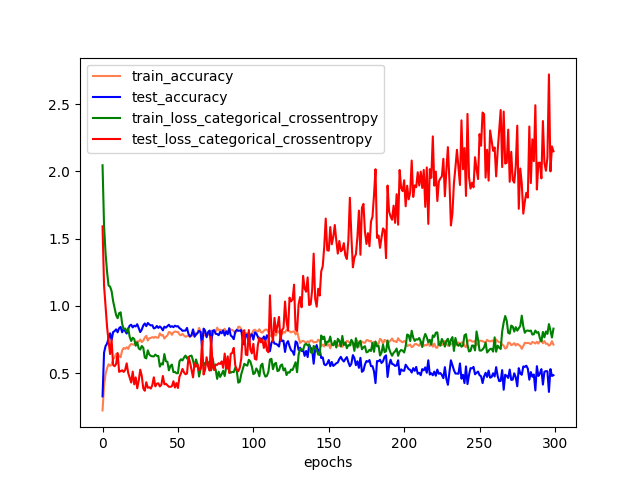
\includegraphics[width=0.66\textwidth]{graphs/model_4.png}
    \caption{Modelul 4}
\end{figure}

Pentru a rezolva problema overfit-ului, am introdus o \emph{regularizare L2} care, conform \cite{l1_l2_regularisation}, ar trebui să ajute în acest caz.
Într-adevăr, situația a fost ameliorată, însă nu a ajutat modelul să prezică mai bine zona în care mă uitam.

\begin{figure}[h]
    \centering
    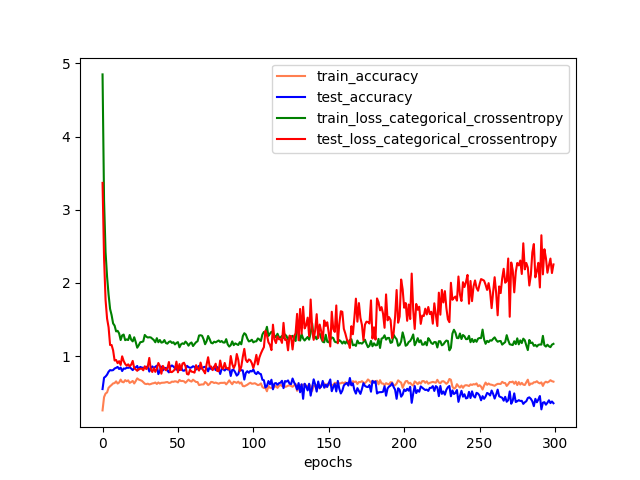
\includegraphics[width=0.49\textwidth]{graphs/model_5.png}
    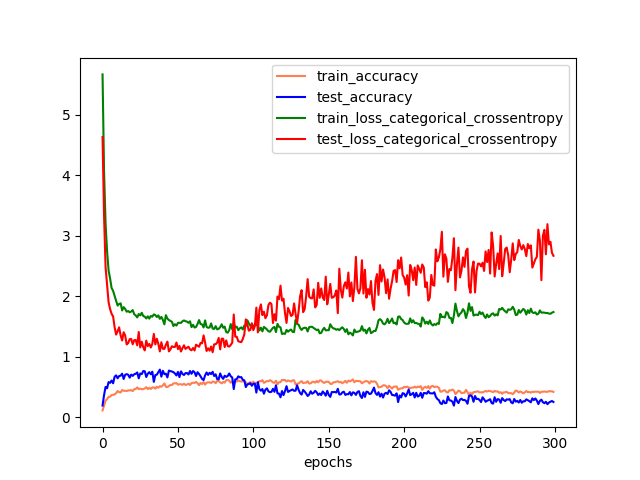
\includegraphics[width=0.49\textwidth]{graphs/model_6.png}
    \caption{Modelele 5 și 6}
\end{figure}

\section{Rețele neuronale de convoluție}
\subsection{Utilizarea întregii feți}

Mai departe am vrut să experimentez cu rețelele convoluționale și am început prin a utiliza fețele extrase din imagini\ref{fig_extracted_faces}, pe o grilă de dimensiune 2x2 \ref{grid-example}.
Din păcate, nu am avut rezultate deloc bune în primă fază.
După o analiză a codului și a datelor, am descoperit că aveam o problemă în cod și că datele nu erau normalizate, fapt care împiedica rețeaua din a învăța.
Am rezolvat această problemă și am continuat experimentarea.


Iată arhitectura cu care am obținut rezultatele ce urmează a fi prezentate:

\label{cnn_first_architecture}
\begin{lstlisting}[language=Python, caption=Prima arhitectură CNN]
model = Sequential()
model.add(Conv2D(16, kernel_size=(3, 3),
                    input_shape=input_shape))
model.add(MaxPooling2D(pool_size=(2, 2)))
model.add(ReLU())
model.add(Conv2D(32, kernel_size=(3, 3)))
model.add(MaxPooling2D(pool_size=(2, 2)))
model.add(ReLU())
model.add(Flatten())
model.add(Dense(128, activation='relu'))
model.add(Dense(4, activation='softmax'))
# optimizer used
opt = Adam()
\end{lstlisting}

\paragraph{Important}
Pentru primele experimente din această secțiune am folosit doar imaginile în care utilizatorul se uita în colțurile ecranului.
De exemplu, pentru o grilă de dimensiune 3x3, am ales doar imaginile în care eticheta corespunzătoare a imaginii este $0, 2, 6$ sau $8$.
Ultima mențiune este că datele de antrenament reprezintă $80\%$ din mulțimea totală de date, restul fiind date de testare.


Mai jos sunt parametrii de antrenare și rezultatele antrenării:

\begin{center}
    \begin{tabular}{ c | c | c | c | c | c | c }
        \hline
        Experiment & Dim. grilă & Nr. imagini & Epoci & Optimizatori & Rată de învățare & Batch size \\ 
        \hline
        7 & 2x2 & 2184 & 50 & Adam & 0.001 & 32 \\
        \hline
        8 & 3x3 & 1247 & 50 & Adam & 0.001 & 32 \\
        \hline
        9 & 4x4 & 711 & 50 & Adam & 0.001 & 32 \\
        \hline
    \end{tabular}
\end{center}

\begin{figure}[h]
    \centering
    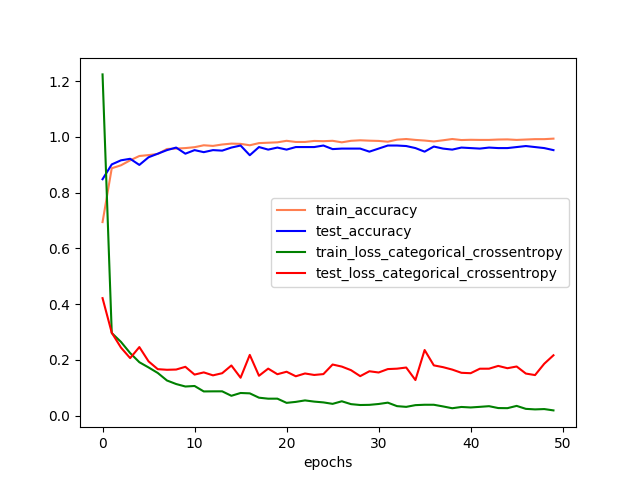
\includegraphics[width=0.32\textwidth]{graphs/model_7.png}
    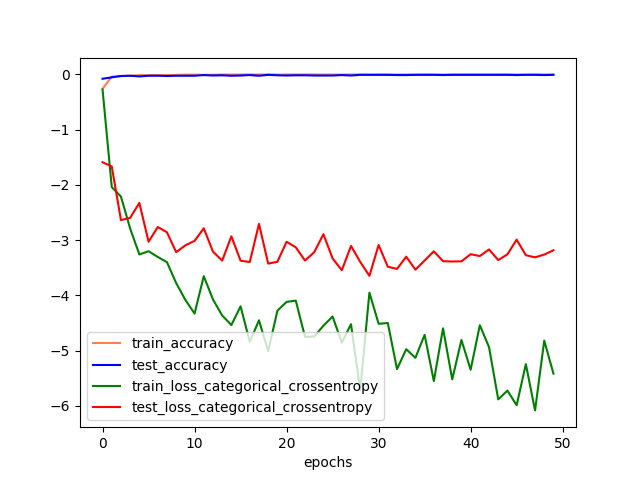
\includegraphics[width=0.32\textwidth]{graphs/model_8.png}
    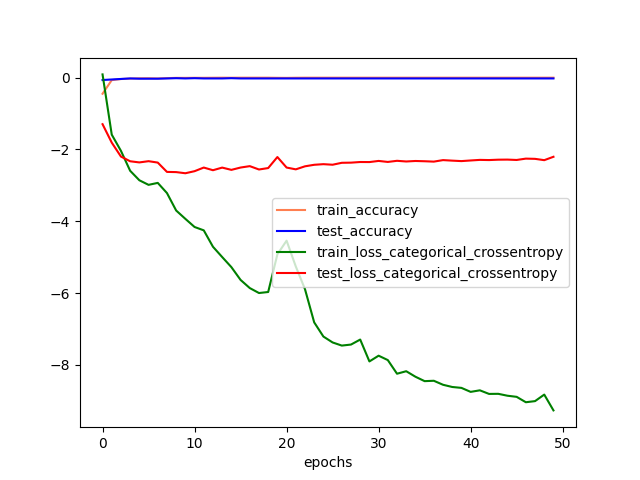
\includegraphics[width=0.32\textwidth]{graphs/model_9.png}
    \caption{Modelele 7, 8 și 9}
\end{figure}

Modelele 8 și 9 au performanțe bune, dar sunt instabile când le folosesc în condiții reale.
Modelul 7 s-a descurcat mai bine.
Dacă mă poziționez la un unghi prielnic față de cameră, acesta poate prezice destul de bine unde privesc.
Acest lucru este probabil datorat faptului că a fost antrenat folosind mai multe date.

Pentru experimentele 10 și 11, am adunat mai multe imagini și am antrenat aceeași arhitectură CNN pe toate datele (nu doar cele corespunzătoare colțurilor ecranului), ceea ce a însemnat 2736 de imagini, pentru grilele de dimensiune 3x3 și 4x4.
Rezultatele au fost mai bune, ceea ce m-a făcut să constat că performanța unui model crește direct proporțional cu dimensiunea mulțimii de date pe care o avem la dispoziție.
Putem vedea de asemenea semne de overfit în aceste modele.

\begin{figure}
    \centering
    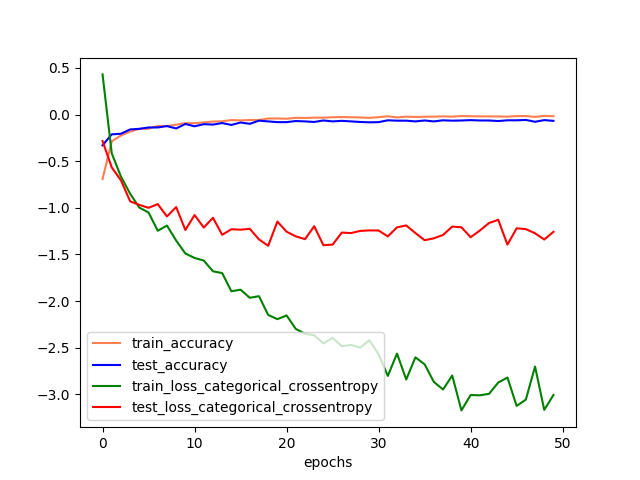
\includegraphics[width=0.49\textwidth]{graphs/model_10.png}
    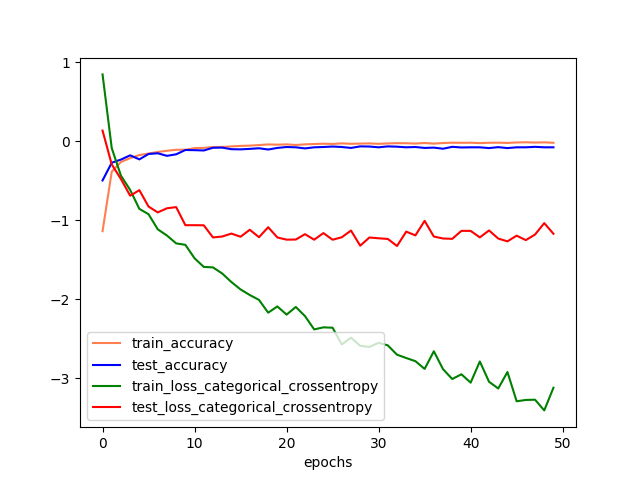
\includegraphics[width=0.49\textwidth]{graphs/model_11.png}
    \caption{Modelele 10 și 11}
\end{figure}

\subsection{Utilizarea ``benzilor oculare'' ca date de antrenament}
Am folosit aceeași arhitectură de rețea convoluțională ca mai sus, dar de această dată folosind doar porțiunile dreptunghiulare care încadrează ambii ochi\ref{fig_extracting_eye_strip}.
Primele modele au fost antrenate doar cu acele imagini în care utilizatorul se uita în colțurile ecranului.

\begin{center}
    \begin{tabular}{ c | c | c | c | c | c | c }
        \hline
        Experiment & Dim. grilă & Nr. imagini & Epoci & Optimizatori & Rată de învățare & Batch size \\ 
        \hline
        12 & 2x2 & 2184 & 50 & Adam & 0.001 & 32 \\
        \hline
        13 & 3x3 & 1247 & 50 & Adam & 0.001 & 32 \\
        \hline
        14 & 4x4 & 711 & 50 & Adam & 0.001 & 32 \\
        \hline
    \end{tabular}
\end{center}

\begin{figure}
    \centering
    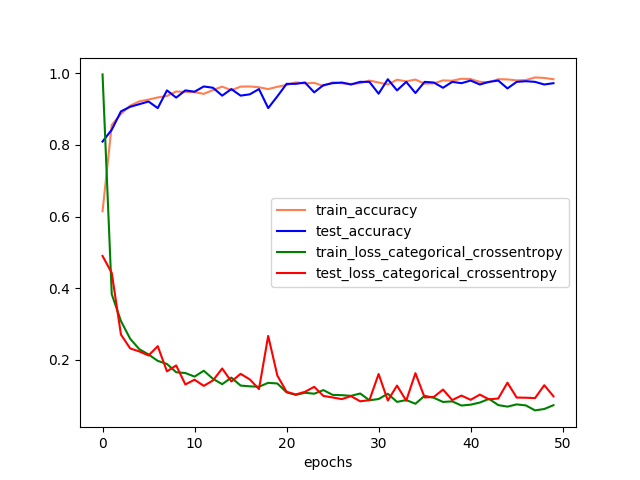
\includegraphics[width=0.32\textwidth]{graphs/model_12.png}
    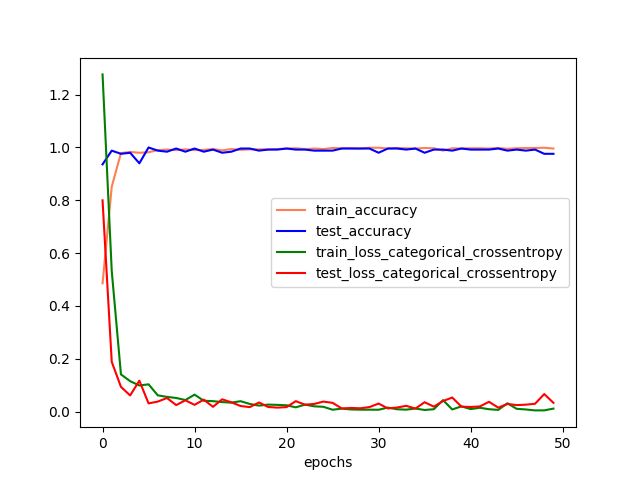
\includegraphics[width=0.32\textwidth]{graphs/model_13.png}
    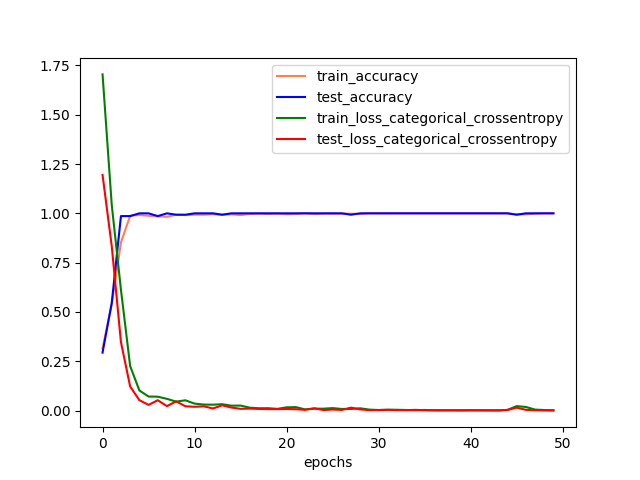
\includegraphics[width=0.32\textwidth]{graphs/model_14.png}
    \caption{Modelele 12, 13 și 14}
\end{figure}

Experimentul 12 a fost unul reușit.
În cadrul acestuia am putut prezice relativ bine unde mă uitam în condiții reale, chiar dacă mă indepărtam sau apropiam de ecran.

Am observat, de asemenea, aceeași tendință de scădere a performanței atunci când modelele sunt antrenate pe mai o mulțime de date mai mică, motiv pentru care experimentele 13 și 14 nu au fost atât de reușite în condiții reale.
Faptul acesta a fost confirmat, întrucât prezicerea a fost mai stabilă, dar tot nu era utilizabilă pentru un produs finit.

\begin{figure}
    \centering
    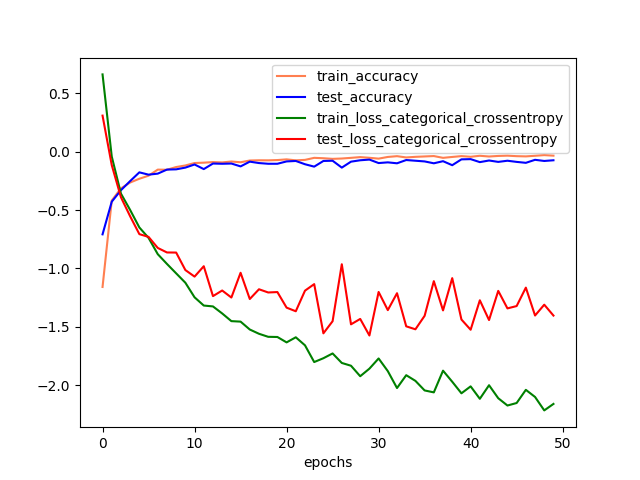
\includegraphics[width=0.49\textwidth]{graphs/model_15.png}
    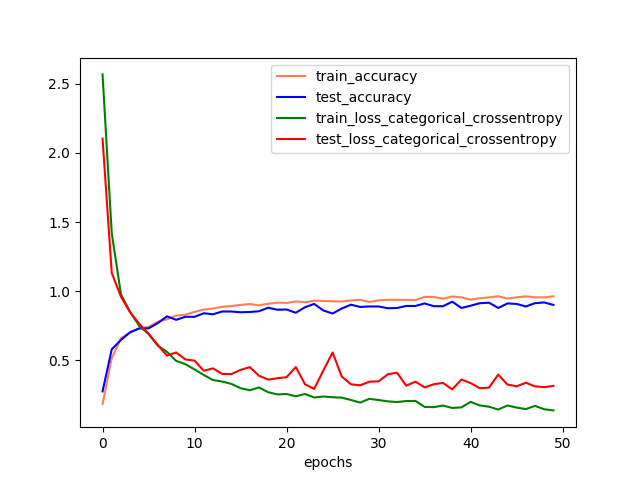
\includegraphics[width=0.49\textwidth]{graphs/model_16.png}
    \caption{Modelele 15 și 16}
\end{figure}

\paragraph{Comentariu intermediar}
Din experimentele prezentate până acum am concluzionat că cea mai bună variantă este folosirea rețelelor convoluționale împreună cu ``benzile oculare''.
Mai mult, atunci când am folosit același algoritm pe mai multe date, modelul realizat a fost mai stabil și a avut performanțe mai bune.
Acest fapt subliniază, din nou, importanța datelor într-un algoritm de învățare automată.

\subsection{Îmbunătățirea arhitecturii CNN}
Experimentele 17–22 au fost rezultatul încercării de a îmbunătăți arhitectura inițială a rețelei de convoluție pe care am folosit-o\ref{cnn_first_architecture}.
Am incercat fie să elimin straturi de convoluție, fie să schimb numărul filtrelor pentru a observa care este comportamentul acesteia.

Am remarcat că atunci când suprimez al doilea strat de convoluție, rețeaua nu mai poate spune atunci când mă uit la anumite celule, deși înainte nu avea probleme în acest sens (spre exemplu celula numărul 2, pe o grilă de dimensiune 3x3).
De asemenea, prin creșterea numărului de filtre de convoluție, performanța a crescut, așadar am decis să continui cu această arhitectură:

\begin{lstlisting}[language=Python, caption=Arhitectura CNN îmbunătățită]
model = Sequential()
model.add(Conv2D(64, kernel_size=(3, 3),
                    input_shape=input_shape))
model.add(MaxPooling2D(pool_size=(2, 2)))
model.add(ReLU())
model.add(Conv2D(128, kernel_size=(3, 3)))
model.add(MaxPooling2D(pool_size=(2, 2)))
model.add(ReLU())
model.add(Flatten())
model.add(Dense(128, activation='relu'))
model.add(Dense(Config.grid_size * Config.grid_size, activation='softmax'))
\end{lstlisting}

\section{Regresie folosind CNN}
O altă idee pe care am avut-o a fost să transform problema inițială, din clasificare în regresie.
Am încercat să prezic exact poziția (coordonatele) la care utilizatorul se uită, iar apoi să o traduc în numărul celulei corespunzătoare.

Pentru acest lucru, am adaptat arhitectura precedentă, astfel încât ultimul strat să fie format din doar 2 neuroni corespunzători coordonatelor (x, y) ale cursorului de pe ecran.
Am schimbat și funcția de activare de pe acest ultim strat într-o funcție liniară $f(x)=x$.
O altă schimbare necesară constă în definirea erorii.
Pentru această regresie am folosit \emph{eroarea medie pătratică} (\emph{Mean Squared Error}, abreviat MSE).
Astfel, formula de calcul a erorii devine:
$$
E = \frac{1}{n} * \sum_{i=1}^{n}{(\hat{y}_{i} – y_i)^2}
$$
unde $y$ este vectorul de coordonate reale (ceea ce trebuie să prezicem), iar $\hat{y}$ este vectorul rezultat, predicția modelului nostru.

Am introdus și o scădere treptată a ratei de învățare (learning rate decay), menită să ajute rețeaua să invețe mai mult și să conveargă mai precis spre parametrii optimi.
În cazul tehnologiei Keras pe care am folosit-o, rata de învățare se adaptează astfel:
\begin{center}
    \lstinline{lr = initial_lr * (1 / (1 + decay * iteration))}
\end{center}
Avantajul unei astfel de tehnici este că putem seta rata de învățare mai mare la început, pentru a invăța mai repede, apoi să o micșorăm pentru a face pași mai mici, dar mai preciși.
Metoda aceasta a dat rezultate pentru un număr mai mare de epoci și a rezultat într-un model care se descurca bine în a atinge obiectivul principal al acestei lucrări.

\begin{center}
    \begin{tabular}{ c | c | c | c | c | c | c }
        \hline
        Experiment & Dim. grilă & Nr. imagini & Epoci & Optimizatori & Rată de învățare & Batch size \\ 
        \hline
        22 & 3x3 & 2736 & 50 & Adam & 0.001 & 32 \\
        \hline
        23 & 3x3 & 2736 & 100 & \vtop{\hbox{\strut Adam}\hbox{\strut decay=$10^{-4}$}} & 0.001 & 32 \\
        \hline
        24 & 3x3 & 2736 & 100 & \vtop{\hbox{\strut Adam}\hbox{\strut decay=$10^{-4}$}} & 0.01 & 32 \\
        \hline
    \end{tabular}
\end{center}

\begin{figure}
    \centering
    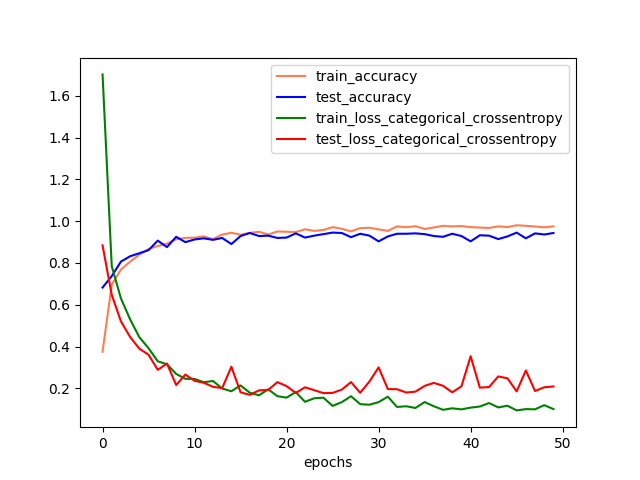
\includegraphics[width=0.32\textwidth]{graphs/model_22.png}
    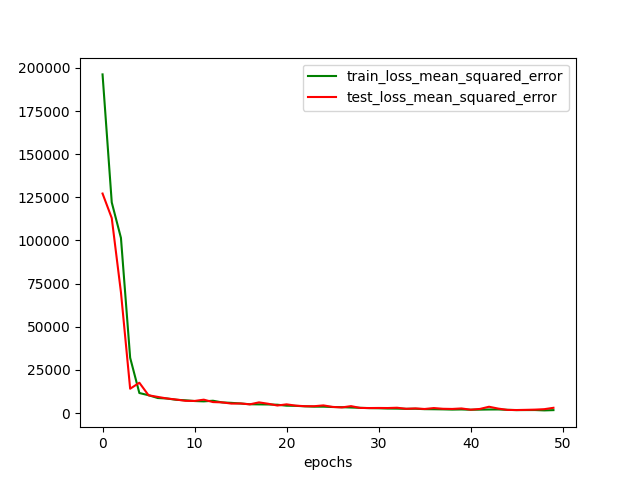
\includegraphics[width=0.32\textwidth]{graphs/model_23.png}
    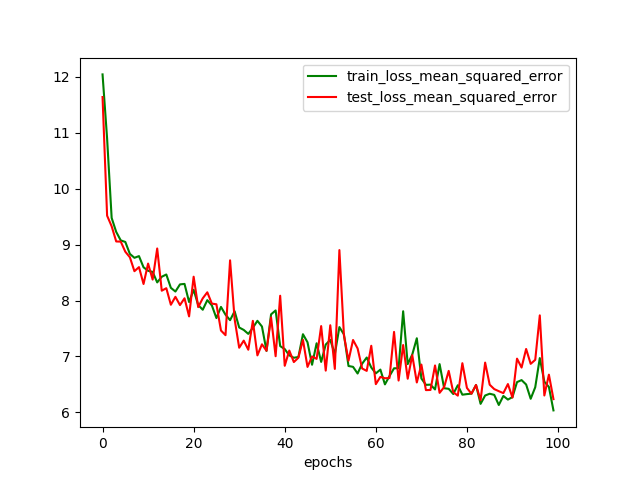
\includegraphics[width=0.32\textwidth]{graphs/model_24.png}
    \caption{Modelele 22, 23 și 24}
\end{figure}

\begin{figure}[h]
    \centering
    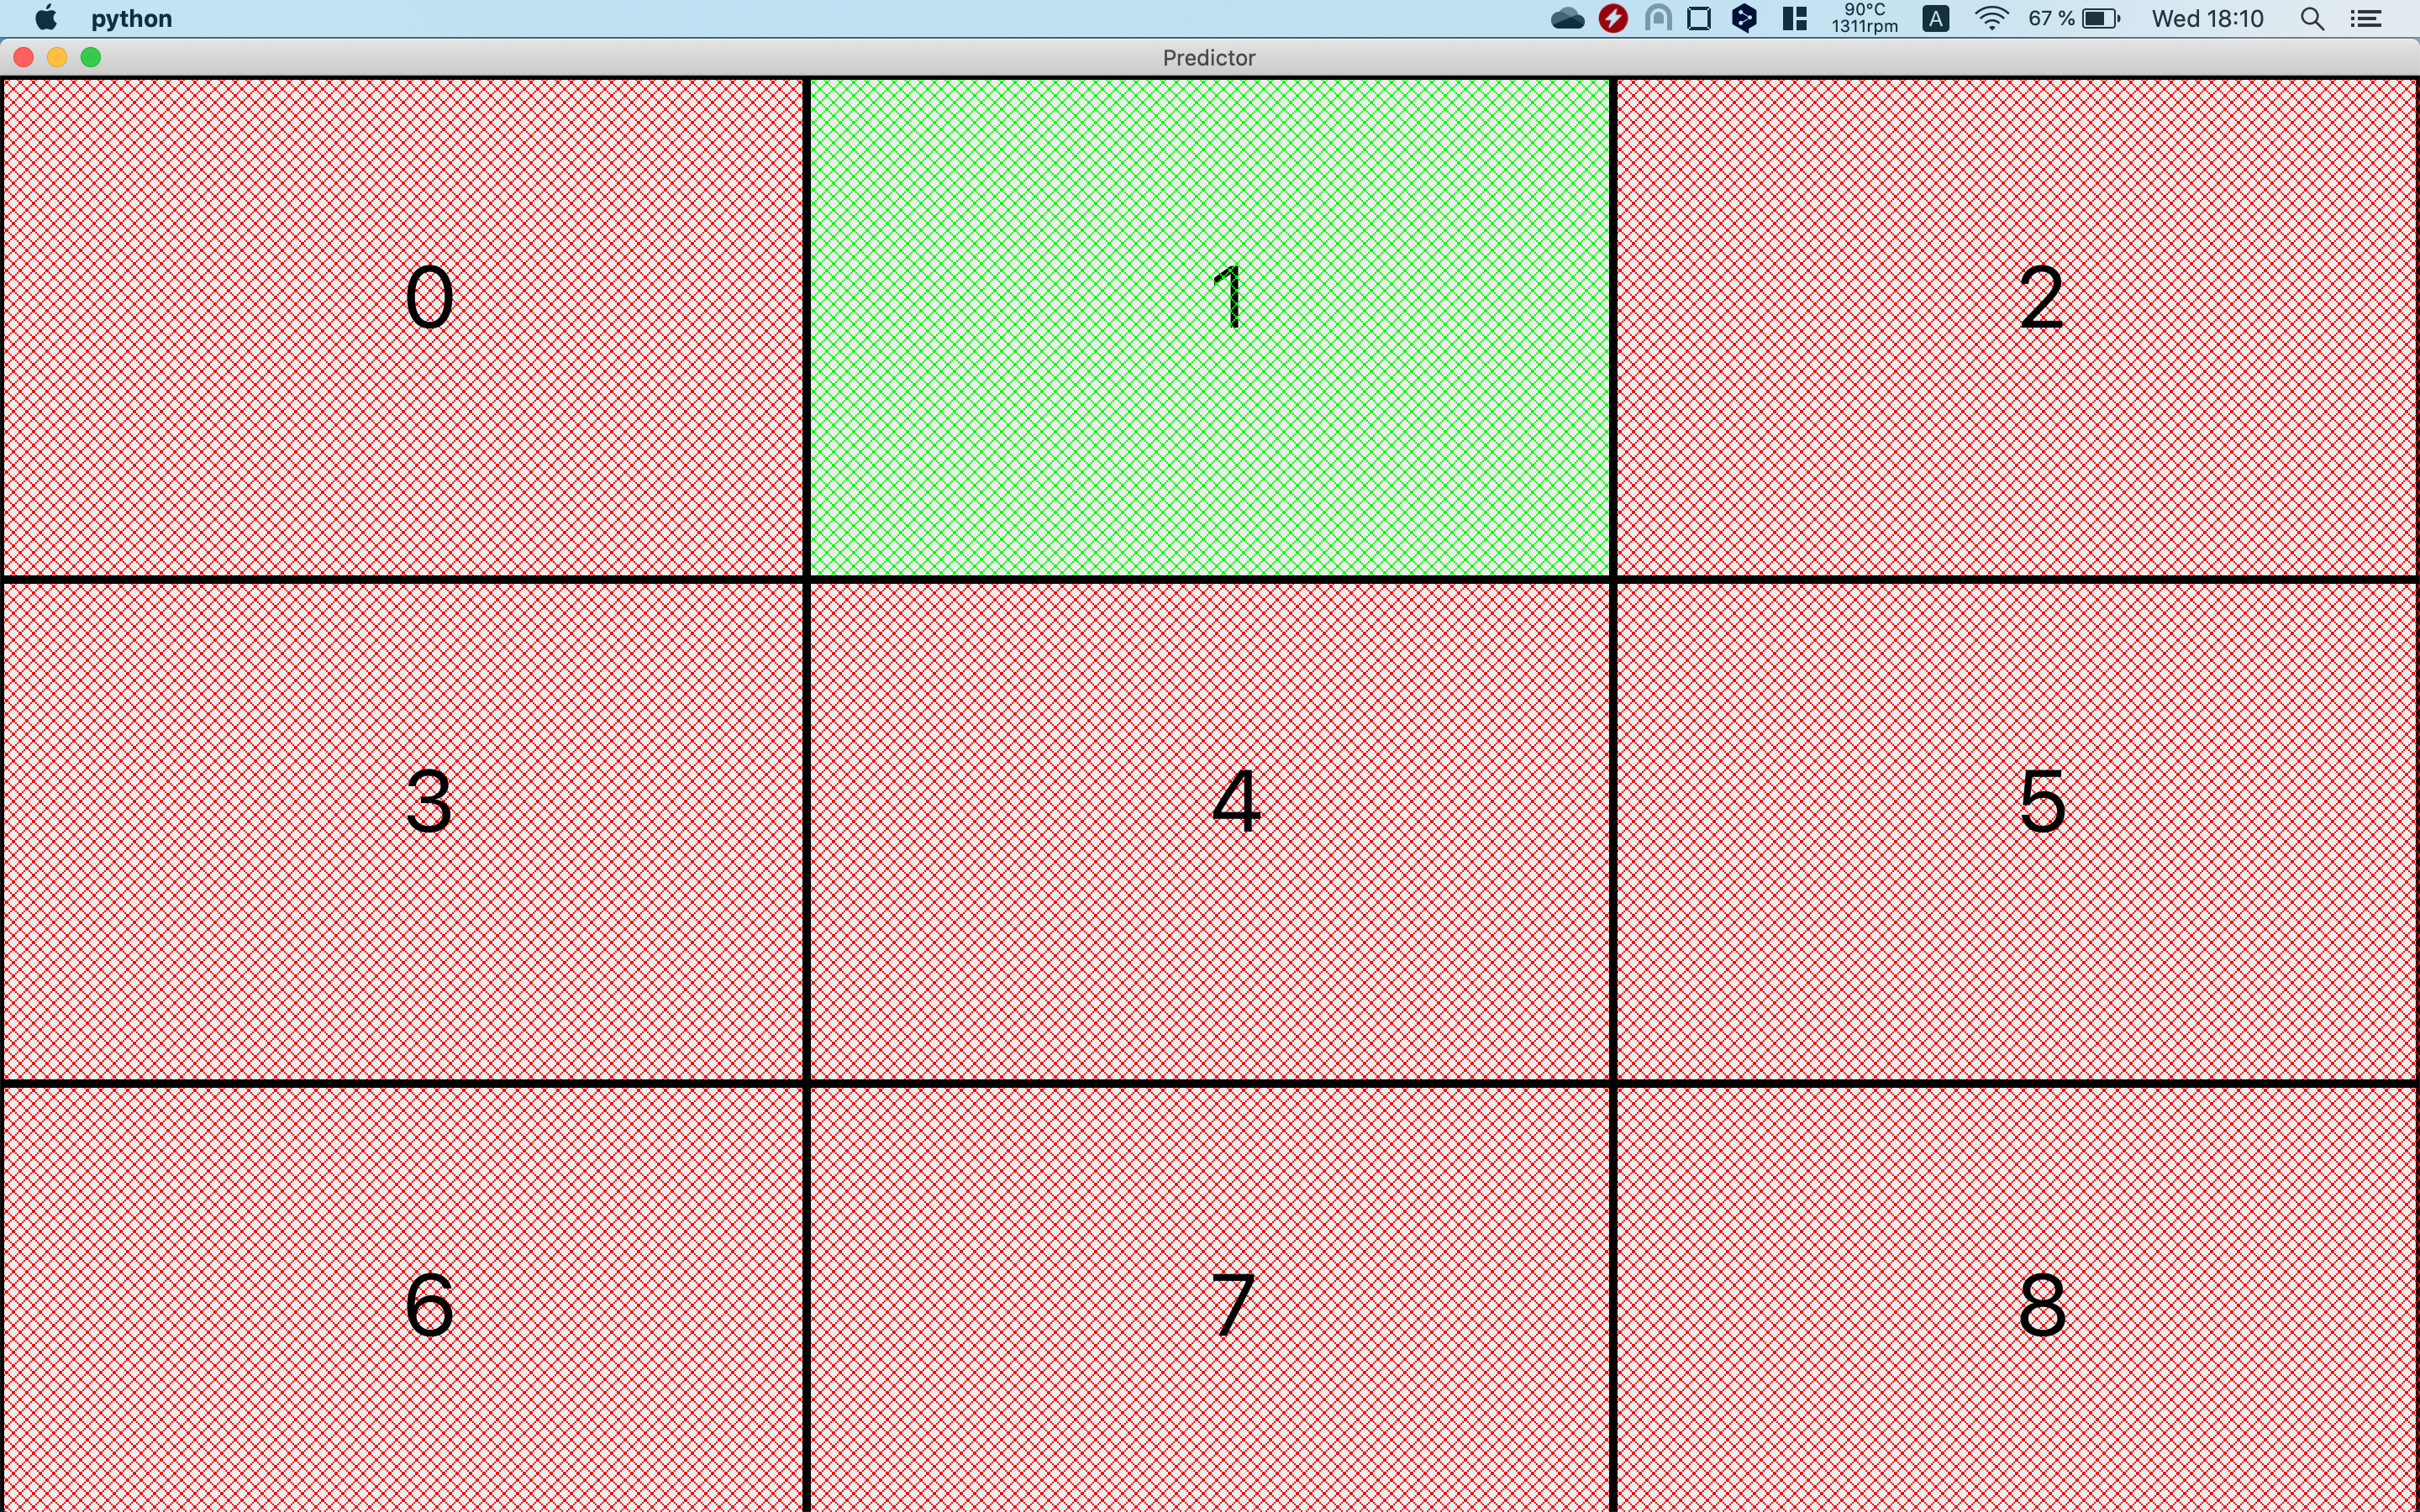
\includegraphics[width=0.49\textwidth]{pred1.png}
    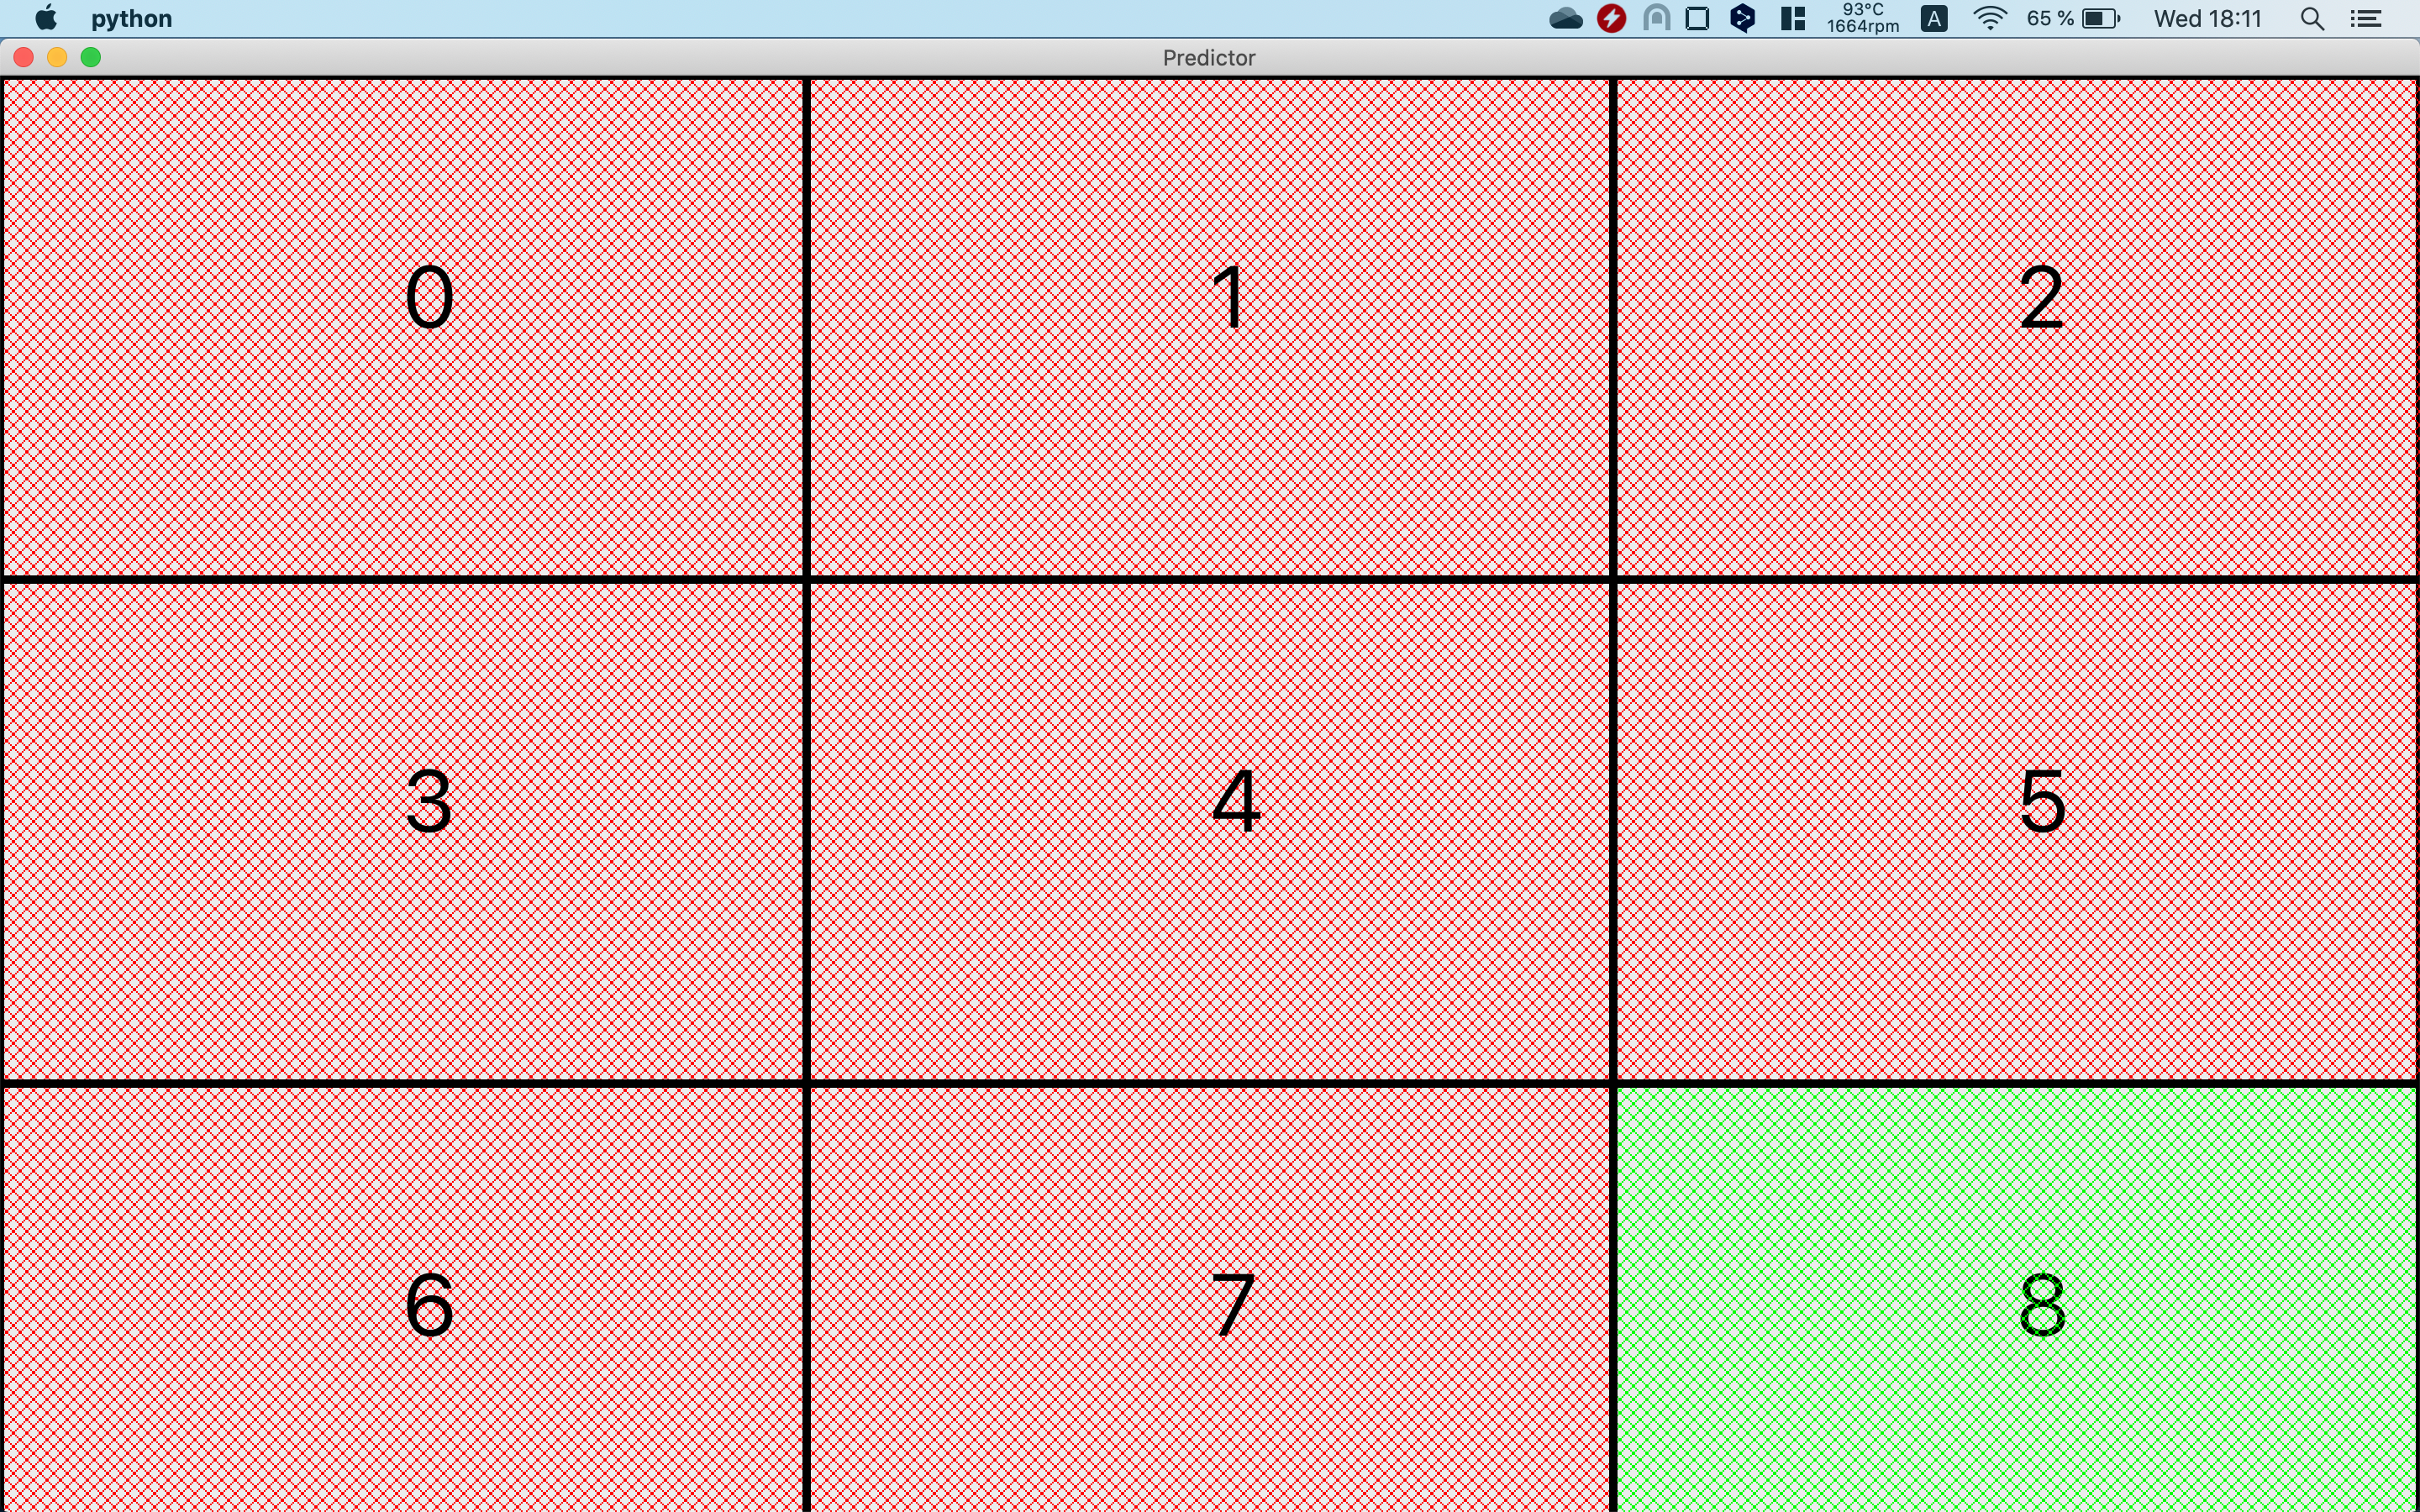
\includegraphics[width=0.49\textwidth]{pred2.png}
    \caption{Utilizarea rețelei CNN pentru urmărirea ochilor}
\end{figure}
    \chapter{Antrenament}
\label{chapter4}
\paragraph{OBSERVAȚIE}
Valorile de pe axa verticală a graficelor prezentate în acest capitol au fost logaritmate.
Acest lucru a ajutat la o vizualizare mai bună a graficelor în care se analizează evoluția antrenării unui model.

\begin{figure}[H]
    \centering
    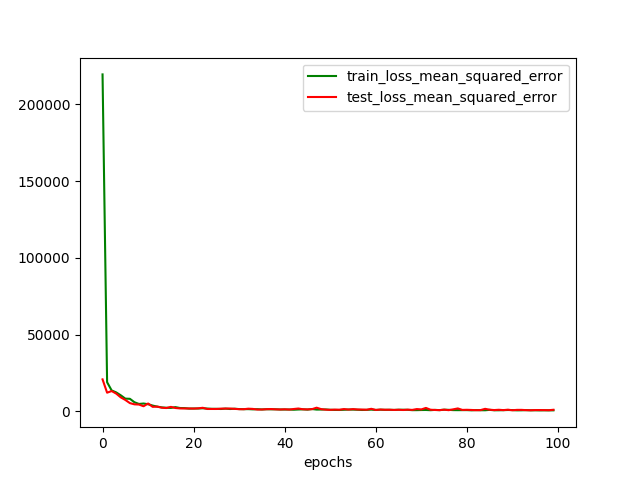
\includegraphics[width=0.49\textwidth]{graph_before_log.png}
    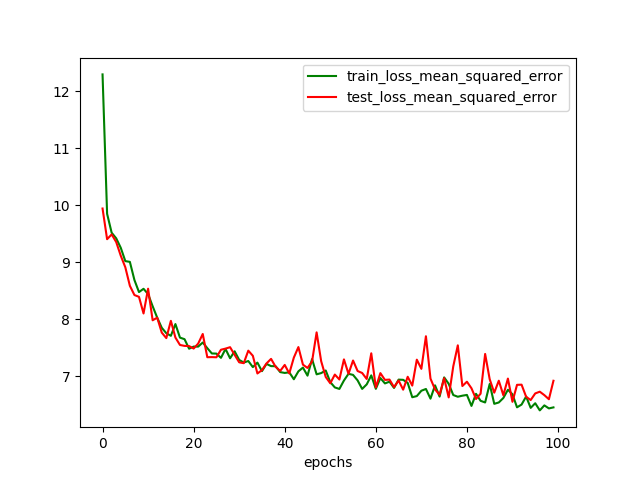
\includegraphics[width=0.49\textwidth]{graph_after_log.png}
    \caption{Graficul aceluiași model, înainte și după logaritmarea valorilor de pe axa verticală}
\end{figure}

Modelele au fost antrenate folosind \emph{framework-ul} Keras.
Dacă valoarea unui parametru nu este menționată, atunci valoarea respectivă este cea prestabilită de Keras (versiunea \lstinline{2.2.4}).

\section{Rețele MLP}
Primele experimente pe care le-am efectuat au fost efectuate folosind imaginile din care am extras ochii, pe care apoi i-am convertit în imagini alb-negru (folosind un \emph{adaptive gaussian threshold}) normalizate, așa cum a fost menționat în prima parte a secțiunii de procesare de date\ref{data-processing:eyes}.
De asemenea, am etichetat fiecare imagine cu numărul celulei în care se uita utilizatorul, conform dimensiunii grilei folosite\ref{grid-example}.
Scopul a fost de a prezice, pentru imagini noi, numărul acelei celule.
Iată arhitectură pe care am folosit-o:

\begin{lstlisting}[language=Python, caption=Arhitectura MLP]
model = Sequential([
    Dense(100, input_shape=(n,), kernel_initializer='glorot_uniform'),
    Dropout(0.5),
    ReLU(),
    Dense(128, kernel_initializer='glorot_uniform'),
    Dropout(0.5),
    ReLU(),
    Dense(64, kernel_initializer='glorot_uniform'),
    # Dropout(0.5),
    ReLU(),
    Dense(Config.grid_size * Config.grid_size, activation='softmax')
])
\end{lstlisting}

Fiind o problemă de clasificare, rețeaua trebuie să furnize pentru fiecare zonă a ecranului $z_i$ o probabilitate $p_i$ însemnând probabilitatea ca în acea imagine utilizatorul să privească zona $z$.
Evident, $\sum(p_i) = 1$.
Pentru acest lucru am folosit ca funcție de activare pe ultimul strat funcția softmax, definită prin
$$
\text{softmax}(x_i) = \frac{e^{x_i}}{\sum_j{e^{x_j}}}
$$
unde $x$ este vectorul care coincide valorilor de pe ultimul strat (9 valori pentru o grilă 3x3) înainte de a trece prin funcția de activare softmax.

\section{TODO: despre ReLU \& kernel initializer \& cel mai important categorical crossentropy loss}

\paragraph{OBSERVAȚIE}
Pentru primele experimente din această secțiune am folosit doar imaginile în care utilizatorul se uita în colțurile ecranului.
De exemplu, pentru o grilă de dimensiune 3x3, am ales doar imaginile în care eticheta corespunzătoare a imaginii este $0, 2, 6$ sau $8$.
Ultima mențiune este că datele de antrenament reprezintă $80\%$ din mulțimea totală de date, restul fiind date de testare.

\begin{center}
    \begin{tabular}{ c | c | c | c | c | c | c }
        \hline
        Experiment & Dimensiune & Număr   & Epoci & Optimizator & Rată     & Batch \\ 
                   & grilă      & imagini &       &             & învățare & size  \\ 
        \hline
        1 & 2x2 & 2184 & 300 & Adam & 0.001 & 32 \\
        \hline
        2 & 3x3 & 1247 & 300 & Adam & 0.001 & 32 \\
        \hline
        3 & 4x4 & 711 & 300 & Adam & 0.001 & 32 \\
        \hline
    \end{tabular}
\end{center}

Experimentele 2 și 3 au beneficiat de mai puține imagini de antrenament deoarece, dimensiunea grilei fiind mai mare, imaginile sunt mai dispersate și fiecare celulă are mai puține imagini corespunzătoare ei.
Evident, pentru o grilă 2x2, fiecare imagine se află intr-o celulă din colț (fiind doar 4), deci au fost folosite toate imaginile.

Primul rezultat pe care l-am constatat a fost că doar primul model putea prezice bine zona în care mă uitam.
Rețeaua MLP se descurca cu atât mai bine cu cât deschideam ochii mai mult, întrucât putea realiza mai bine conturul ochiului și să delimiteze pupila.

\begin{figure}[H]
    \centering
    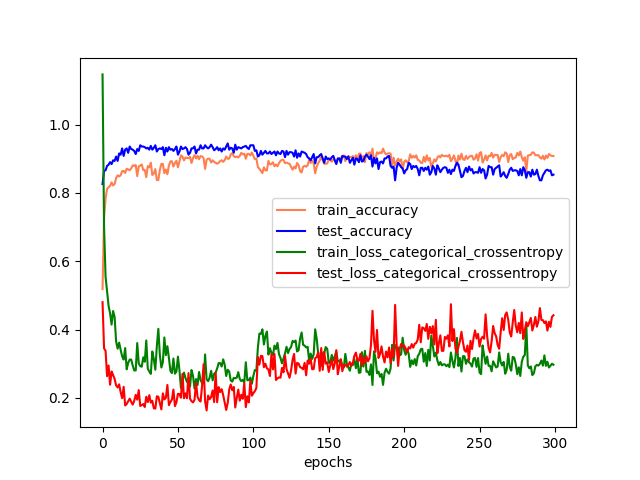
\includegraphics[width=0.49\textwidth]{graphs/model_1.png}
    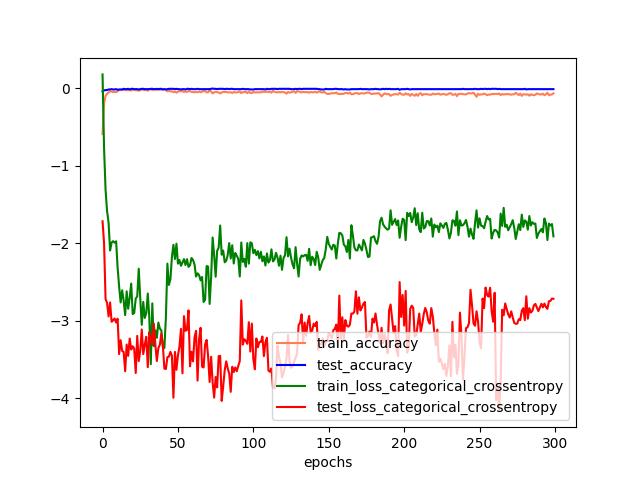
\includegraphics[width=0.49\textwidth]{graphs/model_2.png}
    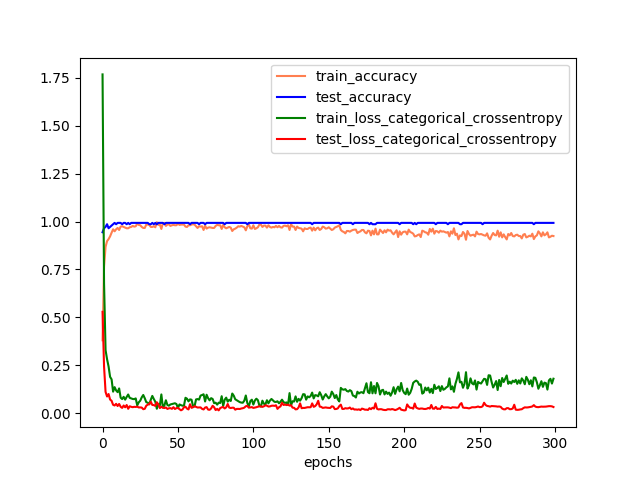
\includegraphics[width=\textwidth]{graphs/model_3.png}
    \caption{Modelele 1, 2 și 3}
\end{figure}

Acuratețea este foarte bună în cele 3 cazuri, însă nu se comportă atât de bine pe imagini noi, într-un mediu diferit.
De asemenea, am constatat ca luminozitatea și modul în care utilizatorul este plasat față de webcam sunt foarte importante și influențează performanța semnificativ.

Un lucru important de observat, care se va regăsi în majoritatea graficelor, sunt acele oscilații, alternanțe ale acurateței, care urcă și coboară.
Stratul \emph{Dropout} este cel care cauzează acest comportament, prin modul în care funcționează: ``by randomly dropping units during training to prevent their co-adaptation'', precum este menționat de \cite{dropout_algorithm}.
Acesta elimină neuroni ai unui strat, în mod aleatoriu, pentru a permite tuturor neuronilor să participe la învățare și să sporească performanța rețelei.
Astfel, atunci când sunt eliminați neuroni ``buni`'', adică aceia care conțin multă informație utilă pentru rezultatul final, performanța (acuratețea, eroarea) pot fi afectate negativ.
Pe de cealaltă parte, atunci când sunt eliminați neuroni care nu ajută foarte mult pentru predicție, performanța nu este afectata prea mult.

Am continuat prin a antrena aceeași rețea, pe o grilă de dimensiune 3x3, dar de data aceasta folosind toate imaginile disponibile.
Totuși, acest lucru nu a ajutat foarte mult și am observat și că după o anumită epocă, rețeaua nu se mai comporta bine pe datele de test și apărea fenomenul de \emph{overfit}.
Acest lucru se poate observa pe graficul modelului 4, unde acuratețea pentru datele de antrenament și cea pentru datele de testare încep să diveargă.

\begin{figure}[h]
    \centering
    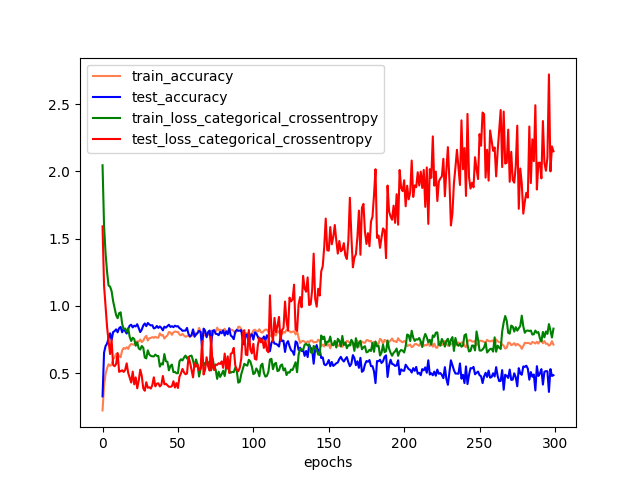
\includegraphics[width=0.66\textwidth]{graphs/model_4.png}
    \caption{Modelul 4. Se observă fenomenul de \emph{overfitting}}
\end{figure}

Pentru a rezolva problema overfit-ului, am introdus o \emph{regularizare L2} care, conform \cite{l1_l2_regularisation}, ar trebui să ajute în acest caz.
Într-adevăr, situația a fost ameliorată, însă nu a ajutat modelul să prezică mai bine zona în care mă uitam.

\begin{figure}[h]
    \centering
    \includegraphics[width=0.49\textwidth]{graphs/model_5.png}
    \includegraphics[width=0.49\textwidth]{graphs/model_6.png}
    \caption{Modelele 5 și 6. \emph{Overfit-ul} este mai puțin pronunțat}
\end{figure}

\section{Rețele neuronale de convoluție}
\subsection{Utilizarea întregii fețe}

Mai departe am vrut să experimentez cu rețelele convoluționale și am început prin a utiliza fețele extrase din imagini \ref{fig_extracted_faces}, pe o grilă de dimensiune 2x2 \ref{grid-example}.
Din păcate, nu am avut rezultate deloc bune în primă fază.
După o analiză a codului și a datelor, am descoperit că aveam o problemă în cod și că datele nu erau normalizate, fapt care împiedica rețeaua din a învăța.
Am rezolvat această problemă și am continuat experimentarea.

Iată arhitectura cu care am obținut rezultatele ce urmează a fi prezentate:

\label{cnn_first_architecture}
\begin{lstlisting}[language=Python, caption=Prima arhitectură CNN]
model = Sequential()
model.add(Conv2D(16, kernel_size=(3, 3),
                    input_shape=input_shape))
model.add(MaxPooling2D(pool_size=(2, 2)))
model.add(ReLU())
model.add(Conv2D(32, kernel_size=(3, 3)))
model.add(MaxPooling2D(pool_size=(2, 2)))
model.add(ReLU())
model.add(Flatten())
model.add(Dense(128, activation='relu'))
model.add(Dense(4, activation='softmax'))
# optimizer used
opt = Adam()
\end{lstlisting}

\paragraph{OBSERVAȚIE}
Pentru primele experimente din această secțiune am folosit doar imaginile în care utilizatorul se uita în colțurile ecranului.
De exemplu, pentru o grilă de dimensiune 3x3, am ales doar imaginile în care eticheta corespunzătoare a imaginii este $0, 2, 6$ sau $8$.
Ultima mențiune este că datele de antrenament reprezintă $80\%$ din mulțimea totală de date, restul fiind date de testare.


Mai jos sunt parametrii de antrenare și rezultatele antrenării:

\begin{center}
    \begin{tabular}{ c | c | c | c | c | c | c }
        \hline
        Experiment & Dimensiune & Număr   & Epoci & Optimizator & Rată     & Batch \\ 
                   & grilă      & imagini &       &             & învățare & size  \\ 
        \hline
        7 & 2x2 & 2184 & 50 & Adam & 0.001 & 32 \\
        \hline
        8 & 3x3 & 1247 & 50 & Adam & 0.001 & 32 \\
        \hline
        9 & 4x4 & 711 & 50 & Adam & 0.001 & 32 \\
        \hline
    \end{tabular}
\end{center}

\begin{figure}[h]
    \centering
    \includegraphics[width=0.32\textwidth]{graphs/model_7.png}
    \includegraphics[width=0.32\textwidth]{graphs/model_8.png}
    \includegraphics[width=0.32\textwidth]{graphs/model_9.png}
    \caption{Modelele 7, 8 și 9}
\end{figure}

Modelele 8 și 9 au performanțe bune, dar sunt instabile când le folosesc în condiții reale.
Modelul 7 s-a descurcat mai bine.
Dacă mă poziționez la un unghi prielnic față de cameră, acesta poate prezice destul de bine unde privesc.
Acest lucru este probabil datorat faptului că a fost antrenat folosind mai multe date.

Pentru experimentele 10 și 11, am adunat mai multe imagini și am antrenat aceeași arhitectură CNN pe toate datele (nu doar cele corespunzătoare colțurilor ecranului), ceea ce a însemnat 2736 de imagini, pentru grilele de dimensiune 3x3 și 4x4.
Rezultatele au fost mai bune în condiții reale de testare, ceea ce m-a făcut să constat că performanța unui model crește direct proporțional cu dimensiunea mulțimii de date pe care o avem la dispoziție.
Putem vedea de asemenea semne de \emph{overfit} în aceste modele.

\begin{figure}
    \centering
    \includegraphics[width=0.49\textwidth]{graphs/model_10.png}
    \includegraphics[width=0.49\textwidth]{graphs/model_11.png}
    \caption{Modelele 10 și 11. Valoarea erorii este mai mare decât modelele 8 și 9 deoarece am folosit mai multe date, fiecare exemplu participând cu o valoare pozitivă la valoarea finală a erorii}
\end{figure}

\subsection{Utilizarea ``benzilor oculare'' ca date de antrenament}
Am folosit aceeași arhitectură de rețea convoluțională ca mai sus, dar de această dată folosind doar porțiunile dreptunghiulare care încadrează ambii ochi \ref{fig_extracting_eye_strip}.
Primele modele au fost antrenate doar cu acele imagini în care utilizatorul se uita în colțurile ecranului.

\begin{center}
    \begin{tabular}{ c | c | c | c | c | c | c }
        \hline
        Experiment & Dimensiune & Număr   & Epoci & Optimizator & Rată     & Batch \\ 
                   & grilă      & imagini &       &             & învățare & size  \\ 
        \hline
        12 & 2x2 & 2184 & 50 & Adam & 0.001 & 32 \\
        \hline
        13 & 3x3 & 1247 & 50 & Adam & 0.001 & 32 \\
        \hline
        14 & 4x4 & 711 & 50 & Adam & 0.001 & 32 \\
        \hline
    \end{tabular}
\end{center}

Experimentul 12 a fost unul reușit.
În cadrul acestuia am putut prezice relativ bine unde mă uitam în condiții reale, chiar dacă mă indepărtam sau apropiam de ecran.

Am observat, de asemenea, aceeași tendință de scădere a performanței atunci când modelele sunt antrenate pe mai o mulțime de date mai mică, motiv pentru care experimentele 13 și 14 nu au fost atât de reușite în condiții reale.
Faptul acesta a fost confirmat, întrucât prezicerea a fost mai stabilă, dar tot nu era utilizabilă pentru un produs finit.

\begin{figure}
    \centering
    \includegraphics[width=0.32\textwidth]{graphs/model_12.png}
    \includegraphics[width=0.32\textwidth]{graphs/model_13.png}
    \includegraphics[width=0.32\textwidth]{graphs/model_14.png}
    \caption{Modelele 12, 13 și 14}
\end{figure}

% \begin{figure}
%     \centering
%     \includegraphics[width=0.49\textwidth]{graphs/model_15.png}
%     \includegraphics[width=0.49\textwidth]{graphs/model_16.png}
%     \caption{Modelele 15 și 16}
% \end{figure}

\paragraph{Comentariu intermediar}
Din experimentele prezentate până acum am concluzionat că cea mai bună variantă este folosirea rețelelor convoluționale împreună cu ``benzile oculare''.
Mai mult, atunci când am folosit același algoritm pe mai multe date, modelul realizat a fost mai stabil și a avut performanțe mai bune.
Acest fapt subliniază, din nou, importanța datelor într-un algoritm de învățare automată.

\subsection{Îmbunătățirea arhitecturii CNN}
Experimentele 17–22 au fost rezultatul încercării de a îmbunătăți arhitectura inițială a rețelei de convoluție pe care am folosit-o \ref{cnn_first_architecture}.
Am incercat fie să elimin straturi de convoluție, fie să schimb numărul filtrelor pentru a observa care este comportamentul acesteia.

Am remarcat că atunci când suprimez al doilea strat de convoluție, rețeaua nu mai poate spune atunci când mă uit la anumite celule, deși înainte nu avea probleme în acest sens (spre exemplu celula numărul 2, pe o grilă de dimensiune 3x3).
De asemenea, prin creșterea numărului de filtre de convoluție, performanța a crescut, așadar am decis să continui cu această arhitectură:

\begin{lstlisting}[language=Python, caption=Arhitectura CNN îmbunătățită]
model = Sequential()
model.add(Conv2D(64, kernel_size=(3, 3),
                    input_shape=input_shape))
model.add(MaxPooling2D(pool_size=(2, 2)))
model.add(ReLU())
model.add(Conv2D(128, kernel_size=(3, 3)))
model.add(MaxPooling2D(pool_size=(2, 2)))
model.add(ReLU())
model.add(Flatten())
model.add(Dense(128, activation='relu'))
model.add(Dense(Config.grid_size * Config.grid_size, activation='softmax'))
\end{lstlisting}

\section{Regresie folosind CNN}
O altă idee pe care am avut-o a fost să transform problema inițială, din clasificare în regresie.
Am încercat să prezic exact poziția (coordonatele) la care utilizatorul se uită, iar apoi să o traduc în numărul celulei corespunzătoare.

Pentru acest lucru, am adaptat arhitectura precedentă, astfel încât ultimul strat să fie format din doar 2 neuroni corespunzători coordonatelor $(x, y)$ ale cursorului de pe ecran.
Am schimbat și funcția de activare de pe acest ultim strat într-o funcție liniară $f(x)=x$.

\begin{lstlisting}[language=Python, caption = Schimbarea ultimului strat pentru problema de regresie]
    model.add(Dense(2, activation='linear'))
\end{lstlisting}

De precizat este faptul că, în acest caz, predicțiile rezultate dintr-o astfel de rețea pot depăși limitele ecranului.
Spre exemplu rețeaua poate prezice că utilizatorul se uită la coordonatele $(-5, 100)$ sau $(2000, 800)$ pentru o rezoluție a ecranului \emph{Full HD}.
În acest caz, am ``reglat'' valorile astfel încât să nu iasă din ecran (de exemplu $(-5, 100)$ devine $(0, 100)$).

O altă schimbare necesară constă în definirea erorii.
Pentru această regresie am folosit \emph{eroarea medie pătratică} (\emph{Mean Squared Error}, abreviat MSE).
Astfel, formula de calcul a erorii devine:
$$
E = \frac{1}{n} * \sum_{i=1}^{n}{(\hat{y}_{i} - y_i)^2}
$$
unde $y$ este vectorul de coordonate reale (ceea ce trebuie să prezicem), iar $\hat{y}$ este vectorul rezultat, predicția modelului nostru.

Am introdus și o scădere treptată a ratei de învățare (learning rate decay), menită să ajute rețeaua să invețe mai mult și să conveargă mai precis spre parametrii optimi.
În cazul tehnologiei Keras pe care am folosit-o, rata de învățare se adaptează astfel:
\begin{lstlisting}[language=Python, caption = Modul în care Keras actualizează rata de învățare]
    lr = initial_lr * (1 / (1 + decay * iteration))
\end{lstlisting}
Avantajul unei astfel de tehnici este că putem seta rata de învățare mai mare la început, pentru a invăța mai repede, apoi să o micșorăm pentru a face pași mai mici, dar mai preciși.
Metoda aceasta a dat rezultate pentru un număr mai mare de epoci și a rezultat într-un model care se descurca bine în a atinge obiectivul principal al acestei lucrări.

\begin{center}
    \begin{tabular}{ c | c | c | c | c | c | c }
        \hline
        Experiment & Dimensiune & Număr   & Epoci & Optimizator & Rată     & Batch \\ 
                   & grilă      & imagini &       &             & învățare & size  \\ 
        \hline
        22 & 3x3 & 2736 & 50 & Adam & 0.001 & 32 \\
        \hline
        23 & 3x3 & 2736 & 100 & \vtop{\hbox{\strut Adam}\hbox{\strut decay=$10^{-4}$}} & 0.001 & 32 \\
        \hline
        24 & 3x3 & 2736 & 100 & \vtop{\hbox{\strut Adam}\hbox{\strut decay=$10^{-4}$}} & 0.01 & 32 \\
        \hline
    \end{tabular}
\end{center}

\begin{figure}[h]
    \centering
    \includegraphics[width=0.32\textwidth]{graphs/model_22.png}
    \includegraphics[width=0.32\textwidth]{graphs/model_23.png}
    \includegraphics[width=0.32\textwidth]{graphs/model_24.png}
    \caption{Modelele 22, 23 și 24}
\end{figure}

\begin{figure}[h]
    \centering
    \includegraphics[width=0.49\textwidth]{pred1.png}
    \includegraphics[width=0.49\textwidth]{pred2.png}
    \caption{Utilizarea rețelei CNN pentru urmărirea ochilor}
\end{figure}
    \chapter{Folosirea modelelor antrenate}
\label{chapter5}
\section{Deplasarea cursorului}
Funcționalitatea de bază a mouse-ului constă în deplasarea cursorului pe ecran.
Am implementat, în primul rând, deplasarea acestuia pe 8 direcții: N, NE, E, SE, S, SV, V, NV.
Dacă utilizatorul vrea să mute cursorul în direcția stânga-sus, atunci acesta va trebui să se uite în acea parte a ecranului (corespunzătoare celulei cu numărul 0 pe o grilă de dimensiune 3x3).
Analog, pentru a-l deplasa în sus, va trebui să se uite pe centrul ecranului în partea de sus (celula cu numărul 1) ș.a.m.d.

\begin{figure}[H]
    \centering
    \includegraphics[width=0.7\textwidth]{cursor_movement.png}
    \caption{Deplasarea cursorului în direcția NV}
\end{figure}

Întrebarea care reiese din paragraful de mai sus este: cum poate solicita utilizatorul deplasarea cursorului?
Fiind o aplicație care se bazează doar pe gesturi ale feței, am decis ca deplasarea cursorului să se realizeze în momentul deschiderii gurii.

Un articol interesant (\cite{driver_drowsiness}) prezintă metode de identificare a oboselii unui șofer.
Un factor cheie este detectarea căscatului, care se rezumă la același gest pe care a trebuit să îl identific și eu.
Articolul propune folosirea reperelor faciale situate pe buze pentru a detecta un raportul de aspect al gurii (\emph{MAR, Mouth Aspect Ratio}).
Formula propusă este:
$$MAR = \frac{|CD| + |EF| + |GH|}{3|AB|}$$

\begin{figure}[H]
    \centering
    \includegraphics[width=0.3\textwidth]{mar.png}
    \caption{Repere faciale folosite pentru a calcula valoarea MAR. Imagine preluată din \cite{driver_drowsiness}}
\end{figure}

Astfel, daca valoarea \emph{MAR} depășește un anumit prag (\emph{MAR threshold}) care este configurabil, atunci aplicația consideră că acesta solicită deplasarea cursorului.
Avantajul configurării acestui prag este că poate fi setat astfel încât utilizatorul să poată și conversa în timp ce aplicația este deschisă, fără a mișca accidental mouse-ul.

\section{Apăsarea butoanelor mouse-ului}
Un gest util ce poate fi folosit în același fel ca mai sus este închiderea ochiului.
Am decis să folosesc închiderea ochiului pentru a simula funcțtiile de ``click stânga'' și ``click dreapta''.
\cite{blink_detection} propune un calcul al raportului de aspect al ochiului (\emph{EAR, Eye Aspect Ratio}) pentru a detecta când o persoană are ochiul închis sau nu.
Formula propusă este:
$$EAR = \frac{||p_2 - p_6|| + ||p_3 - p_5||}{2||p_1 - p_4||}$$

% \begin{figure}[ht]
%     \centering
%     \includegraphics[width=0.5\textwidth]{ear.png}
%     \caption{Detectarea clipirii folosind valoarea EAR. Imagine preluată din \cite{blink_detection}}
% \end{figure}

Când utilizatorul menține ochiul stâng închis pentru un anumit interval de timp $\delta_t$, aplicația va efectua simularea apăsării butonului stâng.
Analog, închiderea ochiului drept va determina simularea apăsării butonului drept.
Intervalul de timp $\delta_t$ a fost folosit pentru a evita apăsarea butoanelor într-un mod inutil atunci când utilizatorul doar clipește.

\begin{figure}[H]
    \centering
    \includegraphics[width=0.49\textwidth]{ear.png}
    \includegraphics[width=0.49\textwidth]{left_click.png}
    \caption{Simularea apăsării butonului stâng de pe mouse folosind valoarea EAR. Prima imagine ilustrează detectarea clipirii și este preluată din \cite{blink_detection}}
\end{figure}
    \chapter{Analiză asupra identificării reperelor faciale}
\label{chapter6}
Utilizând cu succes reperele faciale pentru a localiza și a extrage ochii, ca apoi să folosesc aceste date pentru o rețea convoluțională ca să urmăresc ochii utilizatorului, am devenit interesat de cum funcționează biblioteca Python pe care am folosit-o (dlib) pentru a găsi aceste repere faciale.
Am decis să studiez puțin această problemă și, conform \cite{paper_stacked_hourglass}, metoda \emph{state of the art}, de ultimă oră, pentru detectarea reperelor faciale se bazează pe arhitectura de tipul \emph{Hourglass} care este, într-o formă simplă a ei, o arhitectură de tipul \emph{Autoencoder} (Encoder-Decoder).

\begin{figure}[h]
    \centering
    \includegraphics[width=\textwidth]{hourglass.png}
    \caption{Exemplu de arhitectură Hourglass. Imagine preluată de pe \href{https://medium.com/@sunnerli/simple-introduction-about-hourglass-like-model-11ee7c30138}{Medium}}
\end{figure}

M-am concentrat doar pe prezicerea centrului unui ochi, plecând de la o mulțime de date care conține imagini ale ochiului.
Ca date de antrenament am folosit mulțimea de date pusă la dispoziție pusă la dispoziție de \emph{crowdpupil}\footnote{\url{http://cs.uef.fi/pupoint/}}, care constă în 792 de imagini, fiecare imagine fiind etichetată cu poziția centrului ochiului în acea imagine.

O metodă interesantă pentru identificarea reperelor faciale este prezentată de \cite{ccnn_paper}, care creează o arhitectură compusă din rețele convoluționale puse în cascadă, menite să creeze o \emph{estimare} a acestor puncte și apoi o \emph{rafinare} a lor.
Această metodă se numește \emph{coarse–to–fine estimation}, iar partea de rafinare este tradusă într-o problemă de regresie.

\begin{figure}[H]
    \centering
    \includegraphics[width=\textwidth]{ccnn.png}
    \caption{Arhitectura CCNN propusă de \cite{ccnn_paper}. Consistă într-o combinație între \emph{heatmap estimation} și \emph{landmark regression}.}
\end{figure}

Din căutările pe care le-am efectuat, am descoperit că există două metode de a încerca prezicerea reperelor faciale.
Prima metoda se ocupă cu găsirea coordonatelor exacte $(x, y)$ a fiecărui reper facial prin regresie, iar a doua metodă încearcă construirea unor hărți termografice (\emph{heatmaps}) care codifică acele repere faciale.

Am ales cea de-a doua opțiune, așa că am generat, pentru fiecare imagine a ochiului din mulțimea de date crowdpupil, o hartă termografică care codifică centrul ochiului.
Acest lucru l-am făcut prin a construi o \emph{Distribuție Gaussiană} multivariată (2D), definită prin
$$\mathcal{N}(\mu, \Sigma) = \frac{1}{\sqrt{(2\pi)^{n}|\Sigma|}}exp(-\frac{1}{2}(X-\mu)^T\Sigma^{-1}(X-\mu))$$

În cazul de față am definit $\mu$ și $\Sigma$ astfel:
$$\mu = (x, y), (x, y)$$
$$\Sigma = (f(r), f(r))$$
$\mu$ fiind coordonatele centrului ochiului iar $r$ raza pupilei.

Am calculat o medie pentru valoarea lui $r$ uitându-mă la o parte din imagini iar apoi am definit $f(r) = 1.5 * r$.
Având acestea definite, am putut codifica centrul ochiului fiecărei imagini:

\begin{figure}[h]
    \centering
    \includegraphics[width=0.32\textwidth]{Img_002_L_2.jpg}
    \includegraphics[width=0.32\textwidth]{h_Img_002_L_2.jpg}
    \caption{Centrul ochiului codificat printr-o hartă termografică}
\end{figure}

Am folosit o formă simplă a arhitecturii Hourglass pentru a încerca reconstruirea acestei hărți termografice.
Arhitectura se bazează pe 2 părți corespunzătoare unei arhitecturi \emph{Encoder–Decoder}.
Prima parte produce o \emph{compresie} a informației, iar a doua parte o \emph{decompresie} pentru a încerca reconstruirea imaginii inițiale.
În acest fel, rețeaua învață să folosească doar acele informații care sunt de folos din imaginea originală și care aduc un plus de informație pentru rezultatul final.
Iată arhitectura pe care am folosit-o:

\begin{lstlisting}[language=python]
class MyCNN(nn.Module):
    def __init__(self, input_size):
        super(MyCNN, self).__init__()
        ## eye image -> encoder -> decoder -> heatmap
        filters = [16, 32, 64, 128]
        # starting encoding
        self.layer1 = nn.Sequential(
            nn.Conv2d(1, filters[0], kernel_size=3, padding=2),
            nn.MaxPool2d(kernel_size=2, stride=2, padding=1),
            nn.ReLU(inplace=True),
            nn.BatchNorm2d(filters[0]),
            
            nn.Conv2d(filters[0], filters[1], kernel_size=2, padding=2),
            nn.MaxPool2d(kernel_size=2, stride=2, padding=1),
            nn.ReLU(inplace=True),
            nn.BatchNorm2d(filters[1]),
            
            nn.Conv2d(filters[1], filters[2], kernel_size=3, padding=2),
            nn.MaxPool2d(kernel_size=2, stride=2, padding=1),
            nn.ReLU(inplace=True),
            nn.BatchNorm2d(filters[2]),
            
            nn.Conv2d(filters[2], filters[3], kernel_size=2, padding=1),
            nn.MaxPool2d(kernel_size=2, stride=2, padding=1),
            nn.ReLU(inplace=True),
            nn.BatchNorm2d(filters[3]),
        )
        # encoding done, starting decoding
        self.layer2 = nn.Sequential(
            nn.Upsample(size=(28, 35), mode='bilinear'),
            nn.ConvTranspose2d(filters[3], filters[2], kernel_size=2, stride=1, padding=1),
            nn.ReLU(inplace=True),
            nn.BatchNorm2d(filters[2]),
            
            nn.Upsample(size=(54, 68), mode='bilinear'),
            nn.ConvTranspose2d(filters[2], filters[1], kernel_size=3, stride=1, padding=2),
            nn.ReLU(inplace=True),
            nn.BatchNorm2d(filters[1]),
            
            nn.Upsample(size=(104, 132), mode='bilinear'),
            nn.ConvTranspose2d(filters[1], filters[0], kernel_size=2, stride=1, padding=2),
            nn.ReLU(inplace=True),
            nn.BatchNorm2d(filters[0]),
        
            nn.Upsample(size=(202, 258), mode='bilinear'),
            nn.ConvTranspose2d(filters[0], 1, kernel_size=3, stride=1, padding=2),
            nn.ReLU(inplace=True),
            nn.BatchNorm2d(1),
        )
\end{lstlisting}

Partea de compresie corespunde operației de convoluție care reduce dimensiunea imaginii de la un strat la altul în funcție de parametrii convoluției – spre exemplu pasul (saltul) pe care îl realizează filtrul de convoluție.
În partea de decompresie am folosit operația de \emph{upsampling} care merge înapoi pe pașii convoluției și mărește dimensiunea imaginii, aducându-o la dimensiunea originală (în acest caz imaginile au fost redimensionate la 200x256 pixeli).
Stratul \emph{Upsample} folosește metoda \emph{bilinear} pentru a multiplica pixelii imaginii luând în considerare vecinii acelor pixeli.

Calcularea dimensiunii imaginii rezultată ($W_o$ și $H_o$) după o operație de convoluție se face astfel:
$$W_o = \frac{W - F_w + 2P}{S_w} + 1$$
$$H_o = \frac{H - F_h + 2P}{S_h} + 1$$
unde $(W, H)$ este dimensiunea înainte de operația de convoluție, $(F_w, F_h)$ este dimensiunea filtrului de convoluție, $P$ este \emph{padding-ul} adăugat imaginii iar $(S_w, S_h)$ dimensiunea pasului pe care îl realizează filtrul de convoluție.

Am antrenat rețeaua pentru 12 epoci, folosind optimizatorul \emph{Adam}, iar eroarea a fost calculată folosind \emph{MSE}.
Pentru ultima epocă, media scorului MSE pentru toate datele de test (în jur de 20\% din datele totale) a fost de $8,425983$.

\begin{figure}[H]
    \centering
    \includegraphics[width=\textwidth]{heatmap_predictions.png}
    \caption{Reconstruirea hărților termografice. Prima linie reprezintă adevărul de bază, iar a doua linie rezultatele modelului antrenat}
\end{figure}

Deși rețeaua a reușit să reconstruiască bine hărțile termografice de mai sus, folosind imagini cu mine în condiții reale nu a dat rezultate bune.
Unul dintre motive ar fi rezoluția webcam-ului care nu este foarte bună și imaginile ochilor extrași sunt de o calitate inferioară.
Este interesant de observat în figura de mai jos că rețeaua a putut identifica aproximativ centrul ochiului pe o imagine care conținea fața mea întreagă, deși nu a fost antrenată în acest sens.

\begin{figure}[h]
    \centering
    \includegraphics[width=0.32\textwidth]{heatmap_test.png}
    \includegraphics[width=0.32\textwidth]{heatmap_eye.png}
    \includegraphics[width=0.32\textwidth]{heatmap_result.png}
    \includegraphics[width=0.32\textwidth]{heatmap_original_2.png}
    \includegraphics[width=0.32\textwidth]{heatmap_extracted_2.png}
    \includegraphics[width=0.32\textwidth]{heatmap_result_2.png}
    \caption{Testarea rețelei de tip Hourglass pe imagini cu mine însumi}
\end{figure}

Acest experiment a servit pentru înțelegerea funcționalității bibliotecilor precum dlib.
Experimentul pe care l-am efectuat a fost unul foarte simplu care poate fi extins la a prezice câte o hartă termografică pentru fiecare reper facial (uzual sunt 68) și la a folosi o arhitectură de tip Hourglass mai avansată, care ar folosi, de exemplu, legături reziduale între straturile de convoluție.
Chiar dacă rezultatele finale nu au fost reușite, experimentul m-a ajutat la înțelegerea metodelor \emph{state of the art} pentru identificarea reperelor faciale.
    
    \chapter*{Concluzii} 
\addcontentsline{toc}{chapter}{Concluzii}

Lorem ipsum dolor sit amet, consectetur adipiscing elit, sed do eiusmod tempor incididunt ut labore et dolore magna aliqua. Nunc mattis enim ut tellus elementum sagittis vitae et. Placerat in egestas erat imperdiet sed euismod. Urna id volutpat lacus laoreet non curabitur gravida. Blandit turpis cursus in hac habitasse platea. Eget nunc lobortis mattis aliquam faucibus. Est pellentesque elit ullamcorper dignissim cras tincidunt lobortis feugiat. Viverra maecenas accumsan lacus vel facilisis volutpat est. Non odio euismod lacinia at quis risus sed vulputate odio. Consequat ac felis donec et odio pellentesque diam volutpat commodo. Etiam sit amet nisl purus in. Tortor condimentum lacinia quis vel eros donec. Phasellus egestas tellus rutrum tellus pellentesque eu tincidunt. Aliquam id diam maecenas ultricies mi eget mauris pharetra. Enim eu turpis egestas pretium.
    % \chapter*{Bibliografie} 
\addcontentsline{toc}{chapter}{Bibliografie}
    \printbibliography[title=Bibliografie]

\end{document}
